%%% Local Variables:
%%% mode: latex
%%% TeX-master: t
%%% End:

\documentclass[doctor,openright]{tongjithesis}
% \documentclass[%
%   master|doctor, % mandatory option
%   xetex|pdftex|dvips|dvipdfm, % optional
%   secret,
%   openany|openright,
%   arialtoc,arialtitle]{tongjithesis}

% % 所有其它可能用到的包都统一放到这里了,可以根据自己的实际添加或者删除。
\usepackage{tongjiutils}
\usepackage[top=2.54cm, bottom=2.54cm, left=3.17cm, right=3.17cm]{geometry}


% 你可以在这里修改配置文件中的定义,导言区可以使用中文。
\def\myname{邱君诚}

\begin{document}

% 定义所有的eps文件在 figures 子目录下
\graphicspath{{figures/}}


\frontmatter

%%% Local Variables:
%%% mode: latex
%%% TeX-master: t
%%% End:
\secretlevel{保密} 
\secretyear{2}

\ctitle{基于弹性波模式解耦的全波形反演方法}

% 按照申请工学学位设计。如有其它需要,请修改相应文字。
\makeatletter
  \iftongji@doctor
    \cdegree{博士}
  \else
    \iftongji@master
      \cdegree{理学硕士}
    \fi
  \fi

\makeatother

\cdepartment{同济大学海洋学院}

\cmajorfirst{固体地球物理}

\degtype{理学}

\cauthor{王腾飞}

\cstnr{1110701}

\csupervisor{程玖兵 教授}

% 如果没有副指导老师或者联合指导老师,把各自{}中内容留空即可。

\cassosupervisor{}

\ccosupervisor{}

% 日期自动生成,如果你要自己写就改这个cdate
%\cdate{\CJKdigits{\the\year}年\CJKnumber{\the\month}月}
\makeatletter
  \iftongji@doctor
    \edegree{Doctor of Philosophy}
  \else
    \iftongji@master
      \edegree{Master of Science}
    \fi
  \fi

\makeatother

%\cfunds{自然基金项目(No.123456789)}

%\efunds{(Supported by the Natural Science Foundation of China for\\ Distinguished
%         Young Scholars, Grant No.123456789)}

\etitle{Elastic full waveform inversion based on wave mode decomposition}

\edepartment{School of Ocean and Earth Science}

\edispline{Natural Science}

\emajorfirst{Solid Geophysics}
%\emajorsecond{TONGJILUG}

\eauthor{Tengfei Wang}

\esupervisor{Prof. Jiubing Cheng}

% 这个日期也会自动生成,你要改么?
% \edate{May, 2009}

% 定义中英文摘要和关键字
\begin{cabstract}
	通过地震数据定量地估计介质参数甚至岩石物理参数是探测地球内部结构和勘探油气资源的主要任务。随着计算能力的快速提升以及
	长偏移距、宽方位、宽频带的地震数据采集技术的成熟,旨在估计全波数谱速度模型的全波形反演(FWI)方法
	成为地震勘探中强有力的工具。然而在实际中,FWI无法获得理论上预期的问题解决能力。近几十年来,
	为了解决FWI受到初始模型不够好、数据中缺乏低频导致的周波跳跃(cycle-skipping),克服子波估计不准以及噪音影响等问题的困扰,
	许多学者发展了分频率、分偏移
	距、分散射角等多尺度策略来降低非线性程度。此外,在弹性介质中,
	不同波模式转换及其他多分量数据的复杂性
	进一步增加了反问题的非线性程度,而且
	不同参数扰动的偏导数波场在特定散射角范围内的重叠还会导致参数耦合效应。
	为了重建不同波数谱的模型,本文围绕模式解耦这一数据分离工具,从弹性波全波形反演(EFWI)、弹性波波动方程反射走时反演
	(EWERTI)以及弹性波最小二乘逆时偏移(ELSRTM)出发,尝试恢复高波数、中低波数以及全波数成分的弹性模型参数,进而形成弹性波
	反演中较完整的工作流程体系。

%	在第二章中主要讨论EFWI中模式解耦对压制参数耦合效应的作用。
	EFWI通过最小化观测到的多分量数据与正演模拟数据
	之间的残差来获得高分辨率的地下弹性参数模型。由于Hessian矩阵的显式计算与求逆代价十分
	巨大,实际应用中的大规模问题通常采用梯度类的最优化方法而非基于Hessian的方法。然而,多参数
	反演中的参数耦合效应会引起不同参数间梯度的串扰,进而会严重影响反演的收敛速度与精度。
%	近期,弹性波模式解耦的方法被用来对梯度进行预条件从而降低EFWI过程中的参数耦合
%	问题。
	第二章提出了一种基于模式解耦的EFWI方法,该方法在时间域通过正传
	与解耦的反传波场之间的互相关来获得梯度。文中基于解耦的Frech$\acute{e}t$导数来分析
	Hessian矩阵和分辨率矩阵的性态,并对比常规共轭梯度法、Gauss-Newton法和模式解耦法三者梯度之间的异同来解释模式解耦压制参数耦合的物理机制。
	简单流体饱和模
	型与Marmousi-II模型的数值实例,证明了模式解耦的预条件共轭梯度法(MDPCG)可以降低P-波和S-波速度($V_p$和$V_s$)
	之间的参数耦合,在不涉及Hessian计算的情况下获得快速收敛。

	利用弹性反射波波形反演(ERWI)可以更新中深层模型的中低波数成分,从而为EFWI提供较好的初始模型。
	然而,波形匹配的ERWI也同样会面临周波跳跃的问题。相比波形匹配的目标函数,反射走时目标函数与背景速度模型之间具有
	更加线性的关系。因此第三章中采用弹性波波动方程反射走时反演(EWERTI),
	通过DIW(Dynamic image warping)算法来提取走时残差并以此建立目标函数,
	可以一定程度上回避周波跳跃。
	文中采用基于模式解耦的两步反演策略,首先采用PP波数据反演$V_p$,然后固定反演好的$V_p$通过PS波反演$V_s$。
	地面P/S数据分离可获得不同模式数据残差,空间域弹性波模式解耦则可以对梯度有效地预条件,从而实现$V_p$和$V_s$的分步反演,这将有效降低反演的非线性程度。
	反射波波路径核函数分析解释了解耦的波模式反射路径对压制串扰的重要作用。
%	局部倾角导引正则化约束可以使得反演快速收敛到具有地质意义的模型。
	此外,
	为了降低反演的多解性、保证反演够获得更合理的速度模型,采用包含地层倾角信息的成像结果进行局部倾角导
	引正则化来确保反演获得更符合地质意义的速度模型。
	文中采用Sigsbee2A模型来
	验证EWERTI方法以及反演策略的有效性,并用EFWI检验EWERTI反演结果的准确性。

	ELSRTM旨在通过拟合反射波振幅信息来反演弹性参数模型的高波数成分,可视为线性的EFWI问题。
	常规ELSRTM通过多次迭代可以压制由于数据缺失、粗网格采样等产生的成像噪音,提高成像分辨率,同时部分地降低参数间的耦合
	效应。模式解耦则可以在计算梯度时通过分离出S波梯度,使得ELSRTM中S波速度扰动的反演接近于单参数反演,降低反演参数耦合及非线性程度
	。由此,针对不同的参数耦合情况设计了相应
	的反演策略来压制参数耦合。在$V_p$较少受$V_s$耦合影响时,采用梯度解耦双参数同时反演;而在$V_p$与$V_s$强烈相互影响时,先采用解耦通过S波
	反演好$V_s$,然后反演$V_p$,这样可以进一步压制$V_p$所受到的来自$V_s$的耦合影响。
%	另外,由于实际反射数据与Born模拟数据之间存在差异,因此在ELSRTM中最好能匹配反射数据与背景波场之间的残差。

%	为了恢复弹性介质模型中的不同波数成分,本文
	本文针对弹性波反演问题,分别从EFWI,EWERTI以及ELSRTM
	三个方面入手来恢复不同波数成分的弹性参数模型。在常规多尺度策略的基础上,通过空间域模式解耦和地面P/S分离
	获取P或S数据子集来适应反演中的不同需求。根据解耦的P/S波数据在Frech$\acute{e}t$导数、
	Hessian和分辨率矩阵以及Born反射波路径计算中的贡献和影响,设计出适用于不同阶段的梯度预条件方式和多尺度策略,
	从而降低弹性波反演的非线性和参数耦合程度,
	并形成完整的弹性波反演体系,获得从浅部到深部更准确的弹性参数估计。


\end{cabstract}

\ckeywords{全波形反演,Hessian和分辨率矩阵,参数耦合,波动方程反射走时反演,反射波路径核函数,最小平方逆时偏移,弹性波,模式解耦}

\begin{eabstract}
	The primary task of the detection and exploration of the Earth's interior is to estimate the elastic parameters or rock properties
	quantitively
	through the recording data on the surface. With the developement of 
	high-performance computation ability and the
	maturation of wide-azimuth, long-offset and broadband data accquisition 
	technology, full waveform inversion (FWI) becomes a powerful tool to recover the full
	 wavenumber spectrum of the subsurface. However, FWI can not provide the estimated
	model as good as expected. In order to overcome the obstacles such as bad initial models,
	insufficiency of low frequency component in the data, inaccurately estimated source
	wavelet, low sigal/noisy ratio in the data, many researchers developed hierarachical strategies
	by selecting data subsets of different frequency, offset or scattering-angle during the
	inversion.	
	In elastic media, complicated mode conversions and other multicomponent problems further increase the
	nonlinearity of inversion. Besides, in certain angles, the overlapped partial derivative wavefields of  different
	parameter will lead to trade-offs.
	To rebuild the model containing different wavenumber spectrum, elastic full waveform
	inversion (EFWI), elastic wave equation 
	reflected traveltime inversion (EWERTI) and elastic least square reverse time
	migration (ELSRTM) are implemented with the help of wave mode decomposition, in which we
	try to recover the low and intermediat wavenumber, 
	the high wavenumber and the full wavenumber spectrum of the elastic model.

Elastic full waveform inversion (EFWI) aims to reduce the misfit between recorded and modelled multi-component
seismic data for deducing a detailed model of elastic parameters in the subsurface.
Because the explicit computation and inversion of the Hessian matrix
is extremely resource intensive,
a gradient-based (rather than Hessian-based) minimization is generally applied for large-scale applications.
However, the multi-parameter trade-off effects cause cross-talks in the computed gradients and
thus severely affect the convergence and the quality of the inverted model.
%Recently, preconditioning the gradients based on elastic wave mode decomposition
%has been suggested for mitigating the parameter trade-offs in the EFWI process.
In the second chapter, we propose a mode decomposition (MD)-based EFWI approach, in which the preconditioned gradients
are obtained through the cross-correlation of the forward and
decomposed adjoint wavefields in the time domain.
Based on the decomposed Frech{$\acute{e}$}t derivatives,
we explain the mechanism of this approach through analyses of Hessian and resolution matrices
and comparisons with the Gauss-Newton gradients.
Numerical examples of a simple fluid-saturated model and the Marmousi-II model
demonstrate that the MD-based preconditioned conjugate-gradient approach
can mitigate the trade-off between the P- and S-wave velocities and achieve fast
convergence without any Hessian-involved calculations.

Elastic reflection waveform inversion (ERWI) utilize the reflections to update the low and
intermediate wavenumber in the
deeper part of model, which can provide good initial models for EFWI. However, ERWI suffers from
the cycle-skipping problem due to the objective function of waveform fitting. Since taveltime
information relates to the background model more linearly, the cycle-skipping of traveltime
objective function will be less severe
compared with the previous one. Thus, in the third chapter we implement the WERTI by using the $L_2$ norm of the traveltime
residual extracted by the Dynamic image warping (DIW) as objective function.
The reflection kernel analysis shows that mode decomposition can suppress the artifacts in
gradient calculation. 
Besides, the model regularization through local dip-dependent smooth filter ensures the inversion converging to a
geological model. 
Based on that, a two-step inversion strategy is adopted, in which PP reflections are first used to invert $V_p$,
followed by $V_s$ inversion with PS reflections based on the well recoverd $V_p$. P/S
separation of multicomponent seismograms provides P or S recordings while spatial wave mode
decomposition provides P or S wavefields, which help
to  reduce the nonlinearty of inversion effectively.
%The kernel of reflection wavepath proves that mode decomposition can surpress the artifacts in
%the reflection inversion. 
Numerical example of Sigsbee2A model validates the effectiveness of the
algorithms and strategies for elastic WERTI (E-WERTI).
%Numerical example of Sigsbee2A model validates the effectivenss of the 
%algorithms and strategies for EWERTI, whose results also are tested through EFWI.

ELSRTM is a linearized EFWI aimming to fit the waveform of reflections generated by the inverted
high-wavenumber perturbations. 
%Due to the energy difference between Born and reflection data, it is
%more suitable to match the residual between reflection data and the background data during ELSRTM.
LSRTM can suppress the imaging artifacts caused by reduce migration artifacts arising
from limited aperture, coarse sampling, and acquisition gaps. Conventional ELSRTM can sligthly but
not entirely mitigate the parameter trade-offs. 
Nonetheless, mode decomposition
isolates the S-wave part gradient, which makes the inversion of S-wave velocity
perturbation a mono-parameter inversion to help mitigate the trade-offs. In the fourth chapter, we
design different inversion strategies to cope with the different situations. When $V_p$ is little
affected by $V_s$, we invert the two parameter simultaneously with mode decomposition; when $V_p$
and $V_s$ couple with each
other severely, we recommand inverting $V_s$ firstly followed by $V_p$ inversion to further mitigate
the trade-offs from $V_s$ during the $V_p$ inversion.

In this thesis, we focus on the mode-decomposition-based inversion methods to recover the model
containing different wavenumber spectrum. P/S separation of multicomponent data and wave mode
decomposition provide flexible P or S wave data in different stage of inversion.
Investigation of decomposed Frechet derivative, Hessian and resolution matrices and Born reflection
kernel show the different contribution of P or S wave to gradients. Accordingly, hierarchical
strategies are designed to reduce the nonlinearty, trade-off
effects and other problems during inversion and finally rebuild the elastic model from shallow to
deep more effectively. 

\end{eabstract}

%\ckeywords{全波形反演,Hessian和分辨率矩阵,参数耦合,波动方程反射走时反演,反射波路径核函数,最小平方逆时偏移,弹性波,模式解耦}
\ekeywords{Full waveform inversion, Hessian and resolution matrix, parameter trade-off, 
	wave equation reflected traveltime inversion, kernel of reflection wavepath, least-square RTM,
	Elasticity, Mode decomposition}

\makecover


% 目录

\tableofcontents

\begin{denotation}
\item[GNU] GNU's Not Unix /'gnu:/
\item[GFDL] GNU Free Documentation License
\item[GPL] GNU General Public License
\item[FSF] Free Software Foundation
\item[SMP] 对称多处理
\item[API] 应用程序编程接口
\item[$E$] 能量
\item[$m$] 质量
\item[$c$] 光速
\item[$P$] 概率
\item[$T$] 时间
\item[$v$] 速度
\end{denotation}


%\listoffigures

%\listoftables

%\listofequations

%%% 正文
\mainmatter

%%% Local Variables:
%%% mode: latex
%%% TeX-master: t
%%% End:



\chapter{引言}
%\label{cha:intro}
\section{现状}
针对地下介质的定量成像方法对于刻画油气储层,监测CO$_2$注入以及估计近地表土壤和岩石的物理性
质非常有必要。相比于从地震偏移获得的定性化的叠后反射系数,我们更加希望得到定量化的深度域弹
性参数。地震反演旨在采用迭代的优化类方法通过拟合模拟数据与实际观测数据来恢复地下的真实模型。
不同与层析反演方法,例如Luo and Schuster (1991)\citep{luo1991},只采用走时信息,而全波形反演方法(FWI)提供
了更加完整的思路,同时采用走时与振幅信息来反演\cite[]{tarantola:1986}
随着长偏移距、宽方位和宽频带采集的出现,全波形反演已经成为构建速度模型和进行定量地震成像的有效工具\cite{virieux2009overview}。
然而,FWI所需计算量十分巨大,尤其是在三维模型反演中。因此尽管梯度类的局部优化方法并不能保证反演收敛到全局最优解,
但是由于计算代价小其仍然被广泛应用与FWI中。而更能保证收敛的基于Hessian的求解方法\cite{mora:1987,crase1990robust}
由于更昂贵的计算代价则更多被FWI所舍弃。此外,为了减少计算量,我们通常采用声学近似来获得P波速度\cite{ravaut2004multiscale,operto2006crustal}。
但实际中,即使是以P波为主的无模式转换的单分量地震数据而言,声学近似也只能保证运动学信息的准确,振幅信息只有在小角度入射时才有保证。
这也是声波FWI通常需要非常仔细的数据预处理与预条件。总而言之,地震数据中总是包含弹性波的传播,即使在海上勘探中,
声波反演中并不能考虑到由于模式转换带来的能量损失,这就会对声波数据的产生过高拟合从而低估模型中界面反差。

弹性波全波形反演(EFWI)\cite{tarantola:1986}能够从多分量数据中反演地下介质的弹性参数,如P/S-波速度和密度。
尽管其仍然需要很大计算代价,EFWI还是在很多实际数据中获得了应用
\cite{crase1992nonlinear,djikpesse.tarantola:1999,sears:2008,sears:2010,prieux:2013a,prieux:2013b,vigh:2014}。
EFWI的实现方式可以在时间域\cite{shipp:2002},可以在频率域\cite{brossier2009},也可以采用混合的方式在时间域进行正演模拟而在频率域求解
\cite{nihei.li:2007,sirgue:2008}。然而,EFWI中多个参数参与反演会增加反问题的非线性程度,同时也会受到由于不同物理参数之间的串扰带来的反演
中参数耦合的影响\cite{forgues.lambare:1997}。在海洋环境中,尤其是在软海底环境中,由于P-to-
S的转换模式非常弱,基于拖缆或者海底多分量数据的EFWI的非线性程度会变得更严重\cite{sears:2008}。

很多学者注意到参数化方式对缓解参数耦合效应非常重要。通常可以通过调查散射模式或者Hessian算子来选取不同的参数化方式
\cite[]{wu.aki:1985,tarantola:1986,plessix.cao:2011,gholami2013}。另外一个常用的降低非线性程度的方法是采用多尺度的策略
将速度扰动分解为低波数与高波数成分\cite[]{symes.carazzone:1991,bunks1995multiscale,clement:2001,shin.cha:2008,dehoop:2012,
xu:2012,biondi.almomin:2013,ma.hale:2013,warner2016adaptive,alkhalifah2015scattering}。
将声波FWI扩展到弹性介质中学要付出更多的工作。正如Tarantola(1986)\cite{tarantola:1986}所建议的,我们应当先重构出对数据具有主要影响
的参数,然后再重构出对数据有次级影响的参数。Sears(2008)\cite{sears:2008}提出了一个有效的多尺度策略,通过时间窗来选取海底电缆(OBC)
数据中的不同子集来进行多尺度反演。Operto(2013)\cite{operto2013guided}讨论了如何多级地选取不同的数据分量以及不同的参数类型进行反演,从而
控制参数之间的耦合效应并降低反演的非线性。Xu和mcmechan\cite{xu.mcmechan:2014}提出了一个多步长的策略来提高密度模型的反演精度。

解决参数耦合行之有效的一个方法就是反演中考虑Hessian算子。Hessian逆的对角块能够消除几何扩散以及带限效应带来的模糊性,而非对角块能够压制
参数之间的耦合效应\cite[]{pratt1998gauss,fichtner2011hessian,operto2013guided,innanen2014seismic,pan2015estimation}。
为了避免不可承受的Hessian计算和求逆,很多研究工作都旨在找到对Hessian逆的有效近似,例如采用拟Hessian\cite[]{shin2001improved,choi.shin:2008}
或者通过拟牛顿方式迭代构建Hessian核函数,如L-BFGS方法\cite[]{nocedal2006numerical,brossier2009}。
Sheen等人(2006)\cite{sheen:2006}通过互易原理和褶积定理来计算近似Hessian从而实现了时间域的Gauss-Newton (GN) EFWI方法。
Bae等人(2012)\cite{bae:2012}提出了频率域基于GN共轭梯度法的声弹耦合FWI。
Pratt(1998)\cite{pratt1998gauss}采用“虚震源”引起的偏导数波场的概念解释了梯度与Hessian算子的物理含义。参数耦合效应是由于
不同参数的偏导数波场在特定角度范围内的重叠导致的。因此,Wang等人\cite{wang:2015}在EFWI中,通过解耦弹性波波场并在不同阶段分别选取P波与S波
数据来反演不同参数从而压制参数耦合。通过调查解耦之后的P波与S波目标函数,Ren和Liu\cite{ren.liu:2016}证明了波场的解耦可以降低EFWI的非线性程度。
此外,模式解耦也是弹性波逆时偏移中获得具有物理含义成像的关键步骤\cite{yan:2008,wang2016scalar}。

在本文中,我们并未经验性的通过解耦正、反传波场以及地震记录\cite{ren.liu:2016},而是采用了更有物理意义同时更节省计算量的预条件方式,
也即只解耦反传波场。为了简单起见,我们不在正文中考虑密度反演,而是在讨论部分进行部分阐述。首先,通过弹性波Born近似,我们分析了P波速度与S波速度扰动的
辐射模式,并导出了解耦的Frech{$\acute{e}$}t导数或Jacobian矩阵;然后,我们调查了解耦后的P波与S波数据对梯度的贡献并提出了在梯度计算中的交叉项近似。
在此基础上,预条件的梯度可以通过伴随状态法\cite[]{plessix2006}快速有效地计算得到,也即正传波场与解耦后反传波场的零延迟互相关。
然后,为了获得更多物理机制上的认识,我们计算并分析了基于解耦的Hessian和分辨率矩阵,同时也比较了MD预条件后的梯度与GN梯度的异同。
此后,我们通过在流体饱和沙岩模型以及Marmousi-II模型的数值实验证明了基于解耦的EFWI的有效性。
最后,我们给出关于密度反演的简单讨论并获得了一些结论。

\section{弹性波正问题}
\label{sec:forward_problem}
地球的地下模型可以被认为是弹性假设下的弹性介质。地震波波场在弹性介质中传播的控制方程可以写作:
\begin{equation}
	\rho \frac{\partial u^2_i}{\partial t^2}  -
	\frac{\partial}{\partial x_j}\left[c_{ijkl}\frac{\partial u_{k}}{\partial
	x_l}\right]=f_i,
	\label{eq:WE} 
\end{equation}
其中$u_i$和$f_i$ 分别为质点位移矢量的第$i$分量以及体力项;$\rho$为密度;$c_{ijkl}$
为刚度矩阵张量的分量。上述所有的下标取值为从1到3,并且重复下标的Einstein求和规则被默认隐含在其中。
对于各向同性介质而言,刚度矩阵张量满足:
\begin{equation}
	c_{ijkl}=\lambda\delta_{ij}\delta
	_{kl}+\mu(\delta_{ik}\delta _{jl}+\delta _{il}\delta_{jk}),
	\label{Lame}
\end{equation}
其中,$\lambda$和$\mu$为Lam$\acute{e}$系数,$\delta_{ij}$为Kronecker函数。 

根据Born近似,在$\mathbf{x}$ 位置上对刚度系数做一个微小扰动,$\delta
c_{ijkl}(\mathbf{x})$,将会产生一个扰动波场:
\begin{equation}
	\rho \frac{\partial \delta u^2_i}{\partial t^2}  -
	\frac{\partial}{\partial x_j}\left[c^0_{ijkl}\frac{\partial \delta u_{k}}{\partial
	x_l}\right]=\frac{\partial}{\partial
	x_j}\left[\delta c_{ijkl}\frac{\partial
	u^0_{k}}{\partial x_l}\right]. 
	\label{eq:BornApp}
\end{equation}
其中,$\mathbf{u}^0$为在背景介质$c^0_{ijkl}$中满足方程\eqref{eq:WE}
的背景场。上式说明扰动场可看作是入射波场与参数扰动$\delta
c_{ijkl}(\mathbf{x})$相互作用产生的次级源所引发。为了简单起见,本章的公式推导主要在频率域进行,但是大部分的计算操作则在时间域实现。
利用表示定理与散度定理\cite{kamath2016elastic},扰动波场满足:
\begin{equation}
	\delta u_n(\mathbf{r},\omega)=-\int_{\Omega(\mathbf{x})}{\frac{\partial
	u^0_{k}(\mathbf{x},\omega)}{\partial x_l}
	\frac{\partial G_{ni}(\mathbf{r},\mathbf{x},\omega)}{\partial
	x_j} \delta
	c_{ijkl}(\mathbf{x})}
	d\Omega(\mathbf{x}), \quad (n=1,2,3),
	\label{eq:Repre}
\end{equation}
其中,$\omega$表示频率,$G_{ni}(\mathbf{r},\mathbf{x},\omega)$为弹性波背景格林函数表示在$\mathbf{x}$处沿$i$方向的单位体力源
所产生的在$\mathbf{r}$处沿$n$方向的质点位移,$\Omega(\mathbf{x})$为体积积分范围。注意方程\eqref{eq:Repre}只考虑了一阶散射的情况。
刚度系数扰动与速度扰动之间的关系为:
\begin{equation}
        \delta c_{ijkl}=\frac{\partial c_{ijkl}}{\partial V_p}\delta V_p
        +\frac{\partial c_{ijkl}}{\partial V_s}\delta V_s,
        \label{eq:deltaLame}
\end{equation}
以及
\begin{equation}
        \begin{split}
                &\frac{\partial c_{ijkl}}{\partial V_p}=2\rho V_p\delta_{ij}\delta_{kl},\\
                &\frac{\partial c_{ijkl}}{\partial V_s}=2\rho
                V_s(-2\delta_{ij}\delta_{kl}+\delta_{ik}\delta _{jl}+\delta_{il}\delta_{jk}),
        \end{split}
        \label{eq:deltaLame}
\end{equation}
将方程\eqref{eq:Repre}重写为速度参数化方式:
\begin{equation}
        \delta
        u_n(\mathbf{r},\omega)=\int_{\Omega(\mathbf{x})}{\left[J_{n,V_p}(\mathbf{r,x},\omega)\delta
                V_p(\mathbf{x}) +J_{n,V_s}(\mathbf{r,x},\omega)\delta
        V_s(\mathbf{x})\right]
                }
                d\Omega(\mathbf{x}),
        \label{eq:SplitRepre}
\end{equation}
其中
\begin{equation}
        J_{n,M}(\mathbf{r,x},\omega)=
        T_{ij,M}(\mathbf{x},\omega)G_{ni,j}(\mathbf{r,x},\omega), \quad M\in\{V_p,V_s\},
\label{eq:KernelAB}
\end{equation}
并且
\begin{equation}
\begin{split}
                &T_{ij,M}(\mathbf{x},\omega)=\frac{\partial c_{ijkl}}{\partial M}\frac{\partial
                        u^0_{k}(\mathbf{x},\omega)}{\partial x_l},\\ 
                        &G_{ni,j}(\mathbf{r,x},\omega)=\frac{\partial
                                G_{ni}(\mathbf{r},\mathbf{x},\omega)}{\partial x_j},
\end{split}
\label{eq:traction}
\end{equation}
上述中$J_{n,M}$表示速度扰动对应的偏导数波场\cite[]{pratt1998gauss},$T_{ij,M}$ 表示背景波场$u^0$与速度扰动$\delta V_p$ (或 $V_s$)
作用产生的次级震源,$G_{ni,j}$表示格林函数的空间导数。假设模型网格数与接收点个数为L和K,则方程\eqref{eq:KernelAB}可以重写为离散的形式:
\begin{equation}
        \mathbf{J}_{n,M}(\mathbf{x}_l,\mathbf{r}_k)=
        (\mathbf{T}_M(\mathbf{x}_l):\mathbf{G}'(\mathbf{x}_l,\mathbf{r}_k))_n,\quad
        k=1,2,...,K;\quad l=1, 2,...,L,
        \label{eq:EquivFre}
\end{equation}
其中的双点符号代表了以下操作:
\begin{equation}
    (\mathbf{T}_M:\mathbf{G}')_{n}=\sum_{i,j=1}^{3}T_{ij,M}G_{ni,j}.
    \label{eq:contraction}
\end{equation}
这里为了简化表达我们隐藏了下标$n$来代表多分量数据。因此,方程\eqref{eq:SplitRepre}可写成矩阵形式:
\begin{equation}
            \begin{pmatrix}
                        \mathbf{J}_{V_p}&\quad\mathbf{J}_{V_s}
    \end{pmatrix}
    \begin{pmatrix}
       \delta  \mathbf{V}_p\\
       \delta \mathbf{V}_s
    \end{pmatrix}
    =
        \mathbf{\delta u},
        \label{eq:finalMatrix}
\end{equation}
其中$\mathbf{J}_{V_p}$和$\mathbf{J}_{V_s}$为$K\times L$大小的Frech{$\acute{e}$}t导数(Jacobian矩阵),
$\delta \mathbf{V}_p$和$\delta \mathbf{V}_s$为长度为$L$的模型参数向量,$\delta \mathbf{u}$为在接收点位置上的弹性散射波场。
则方程\eqref{eq:finalMatrix}可以简化为:
\begin{equation}
        \mathbf{J}\delta \mathbf{m}
    =
        \mathbf{\delta u},
        \label{eq:finalMatrixshort}
\end{equation}
with $\mathbf{J}=(\mathbf{J}_{V_p}\quad\mathbf{J}_{V_s})$ and
$\delta \mathbf{m}=(\delta\mathbf{V}_p \quad \delta\mathbf{V}_s)^T$.

方程\eqref{eq:finalMatrix}或\eqref{eq:finalMatrixshort}说明Jacobian矩阵与参数扰动向量的乘积即为相应的散射数据响应,而所有该数据响应的
叠加就组成了整个散射波波场。从图\ref{fig:radiationpattern}中展示的散射模式可看出,$\delta V_p$只通过PP模式散射P波数据,而$\delta V_s$
则散射所有模式的P波和S波数据。因此这就很难分辨出散射数据中的P波是来自于哪一类速度扰动($\delta V_p$或$\delta V_s$)。
幸运的是,散射S波则仅仅由$V_s$产生,因而对于单次散射的弹性波数据来讲,耦合效应只会出现在P波的模式中。
反演中的参数耦合效应是由于不同模型参数的偏导数波场在特定角度范围内的重叠导致的\cite{tarantola:1986,operto2013guided}。
所以很自然地,我们采用模式解耦来作为EFWI中降低参数耦合效应的工具。
\begin{figure*}
    \begin{center}
        \subfloat(a){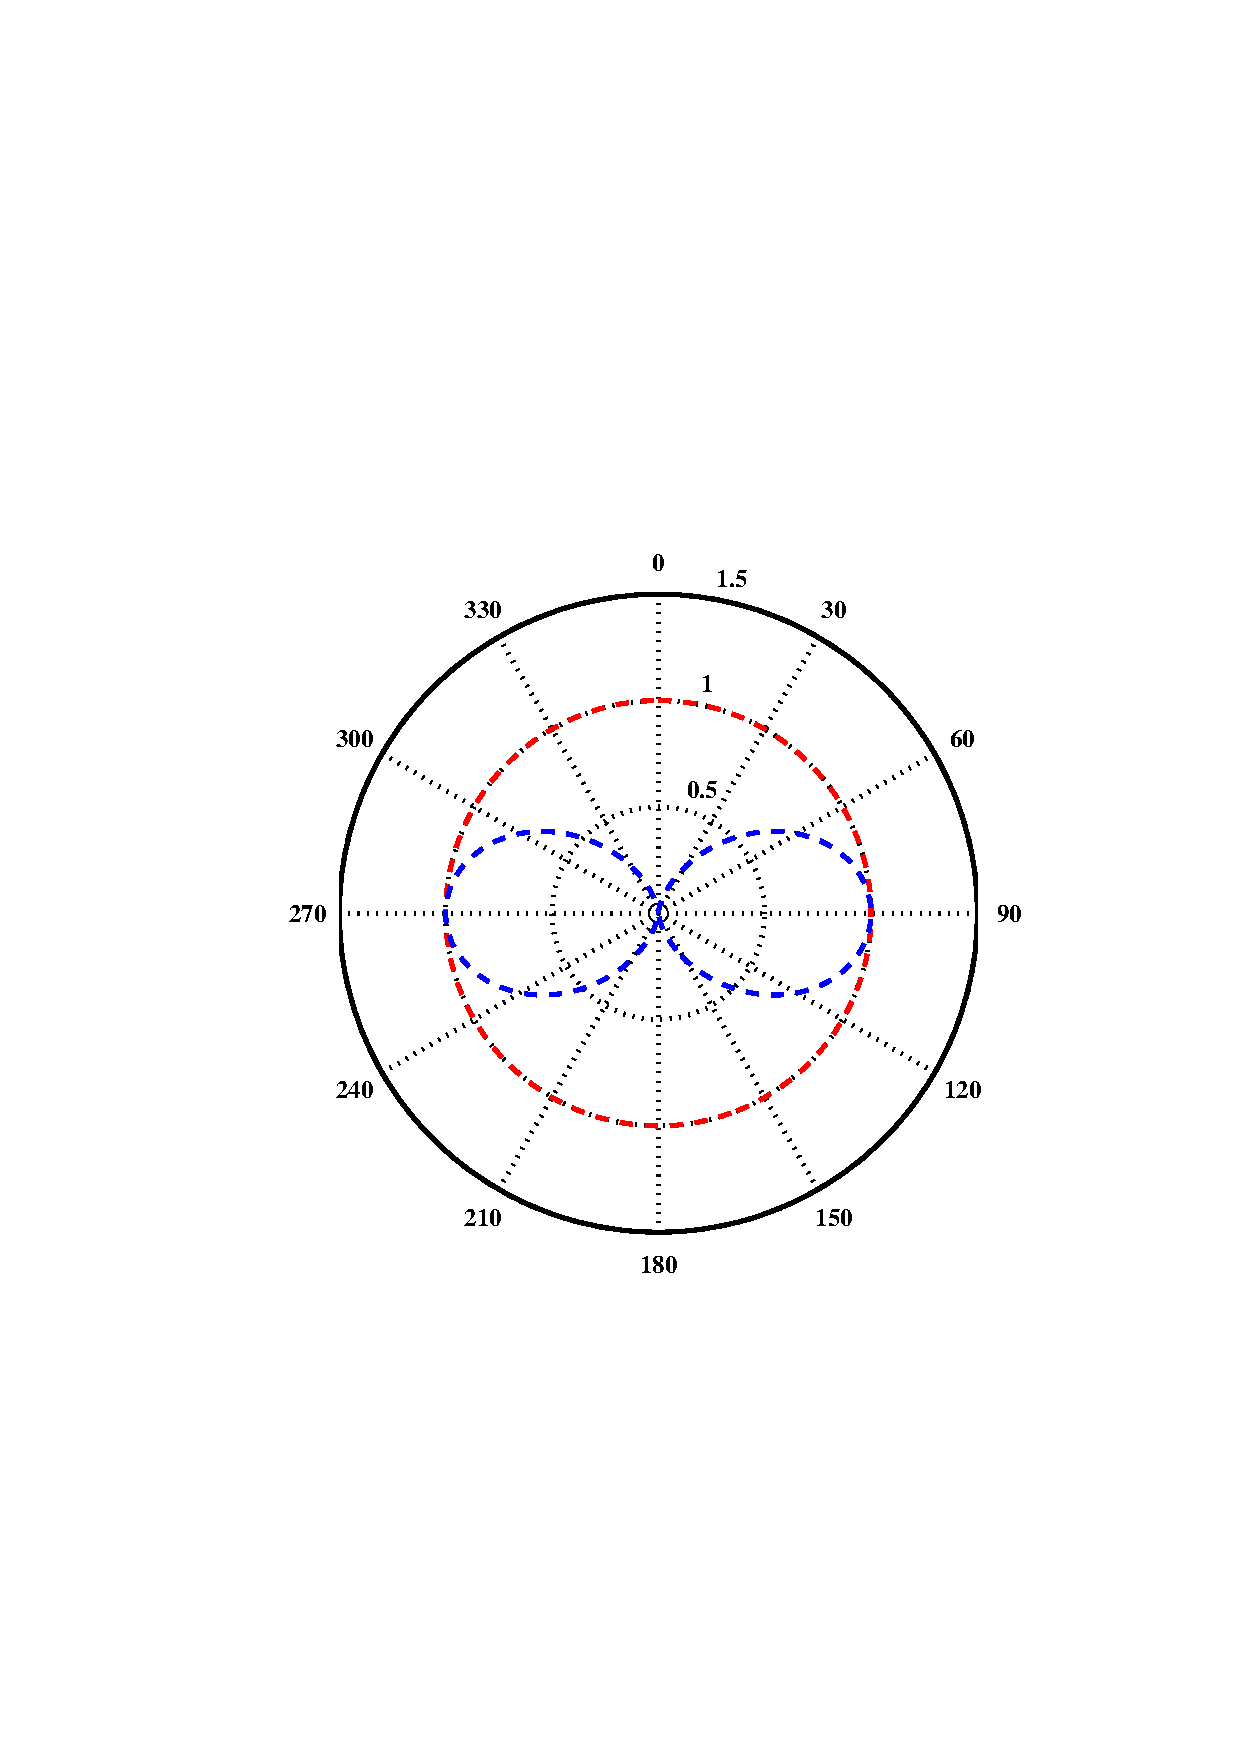
\includegraphics[width=5cm]{radiationpattern/Fig/PP.pdf}}
%        \subfigure{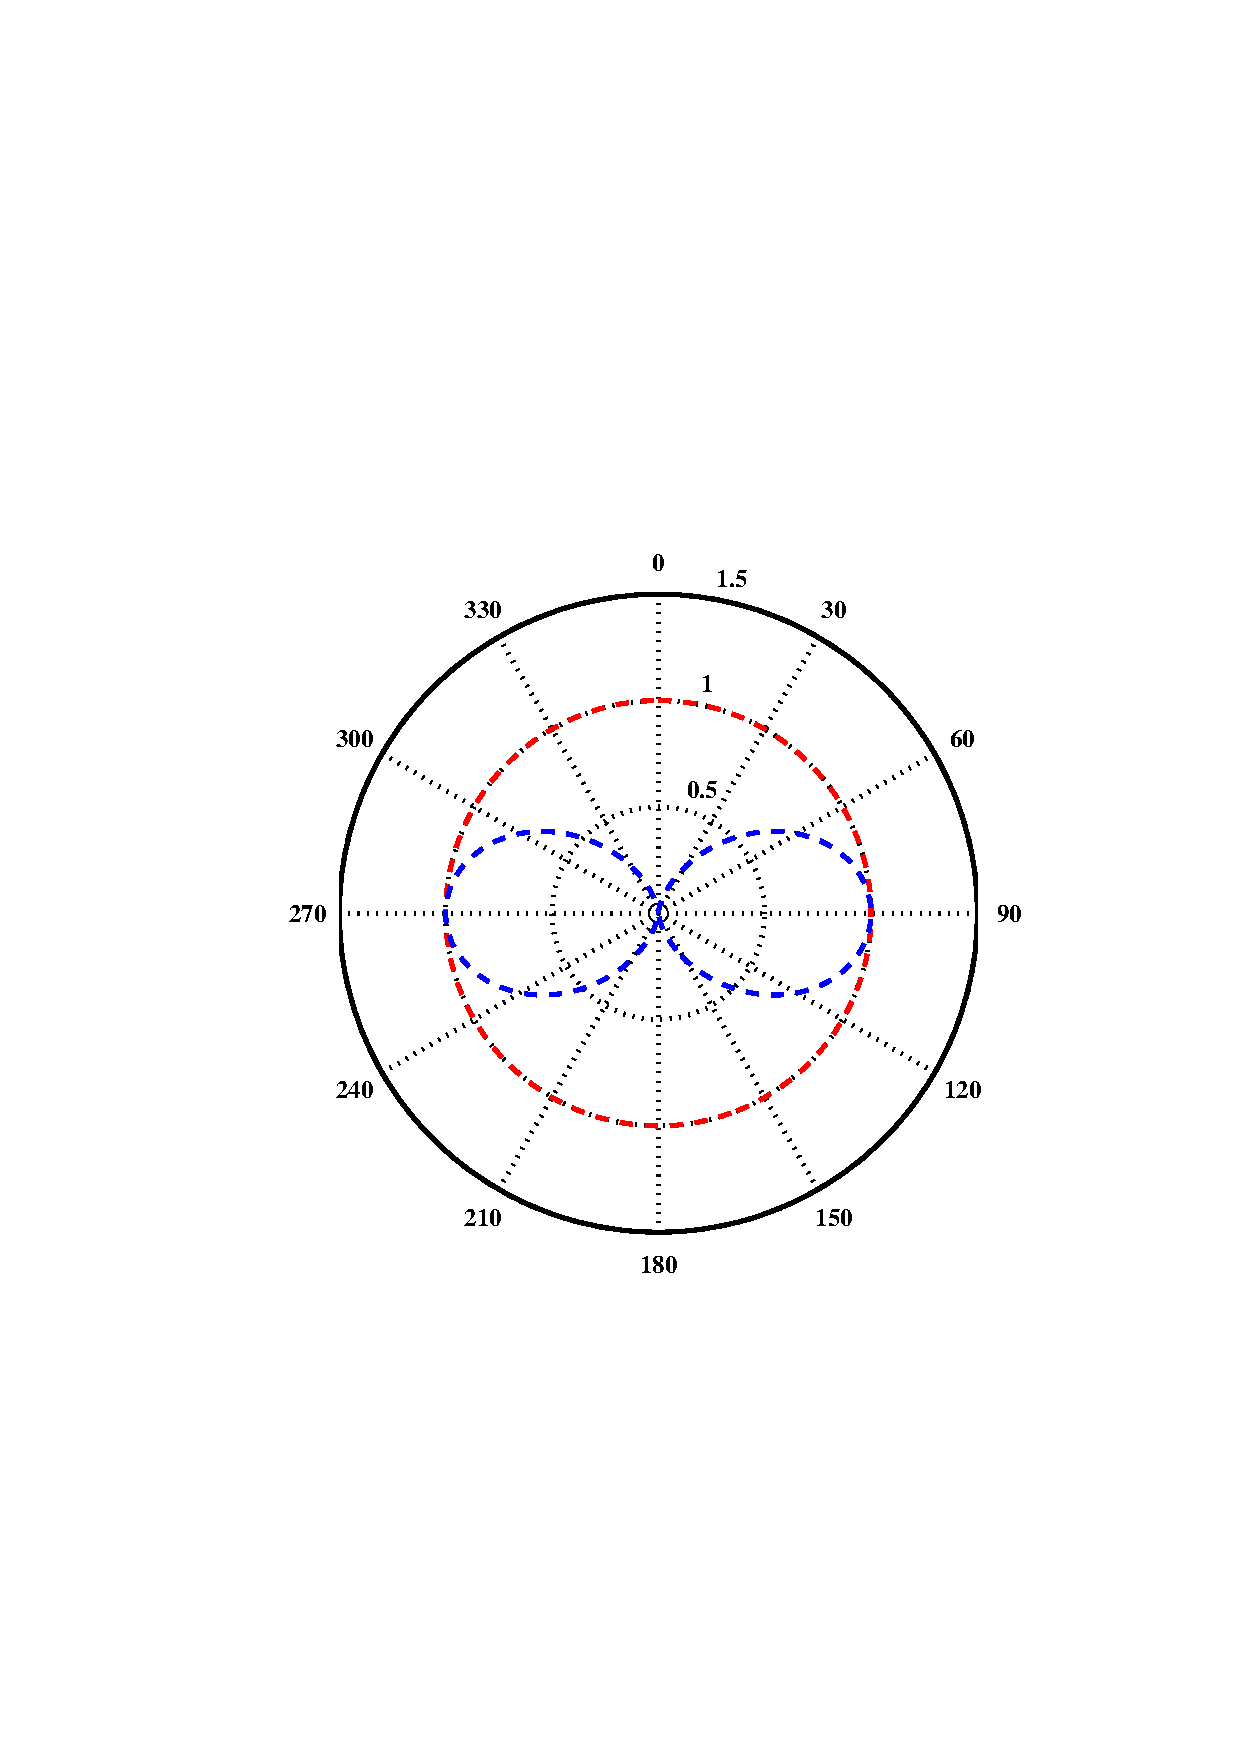
\includegraphics[width=5cm]{radiationpattern/Fig/PP.pdf}}
        \subfloat(b){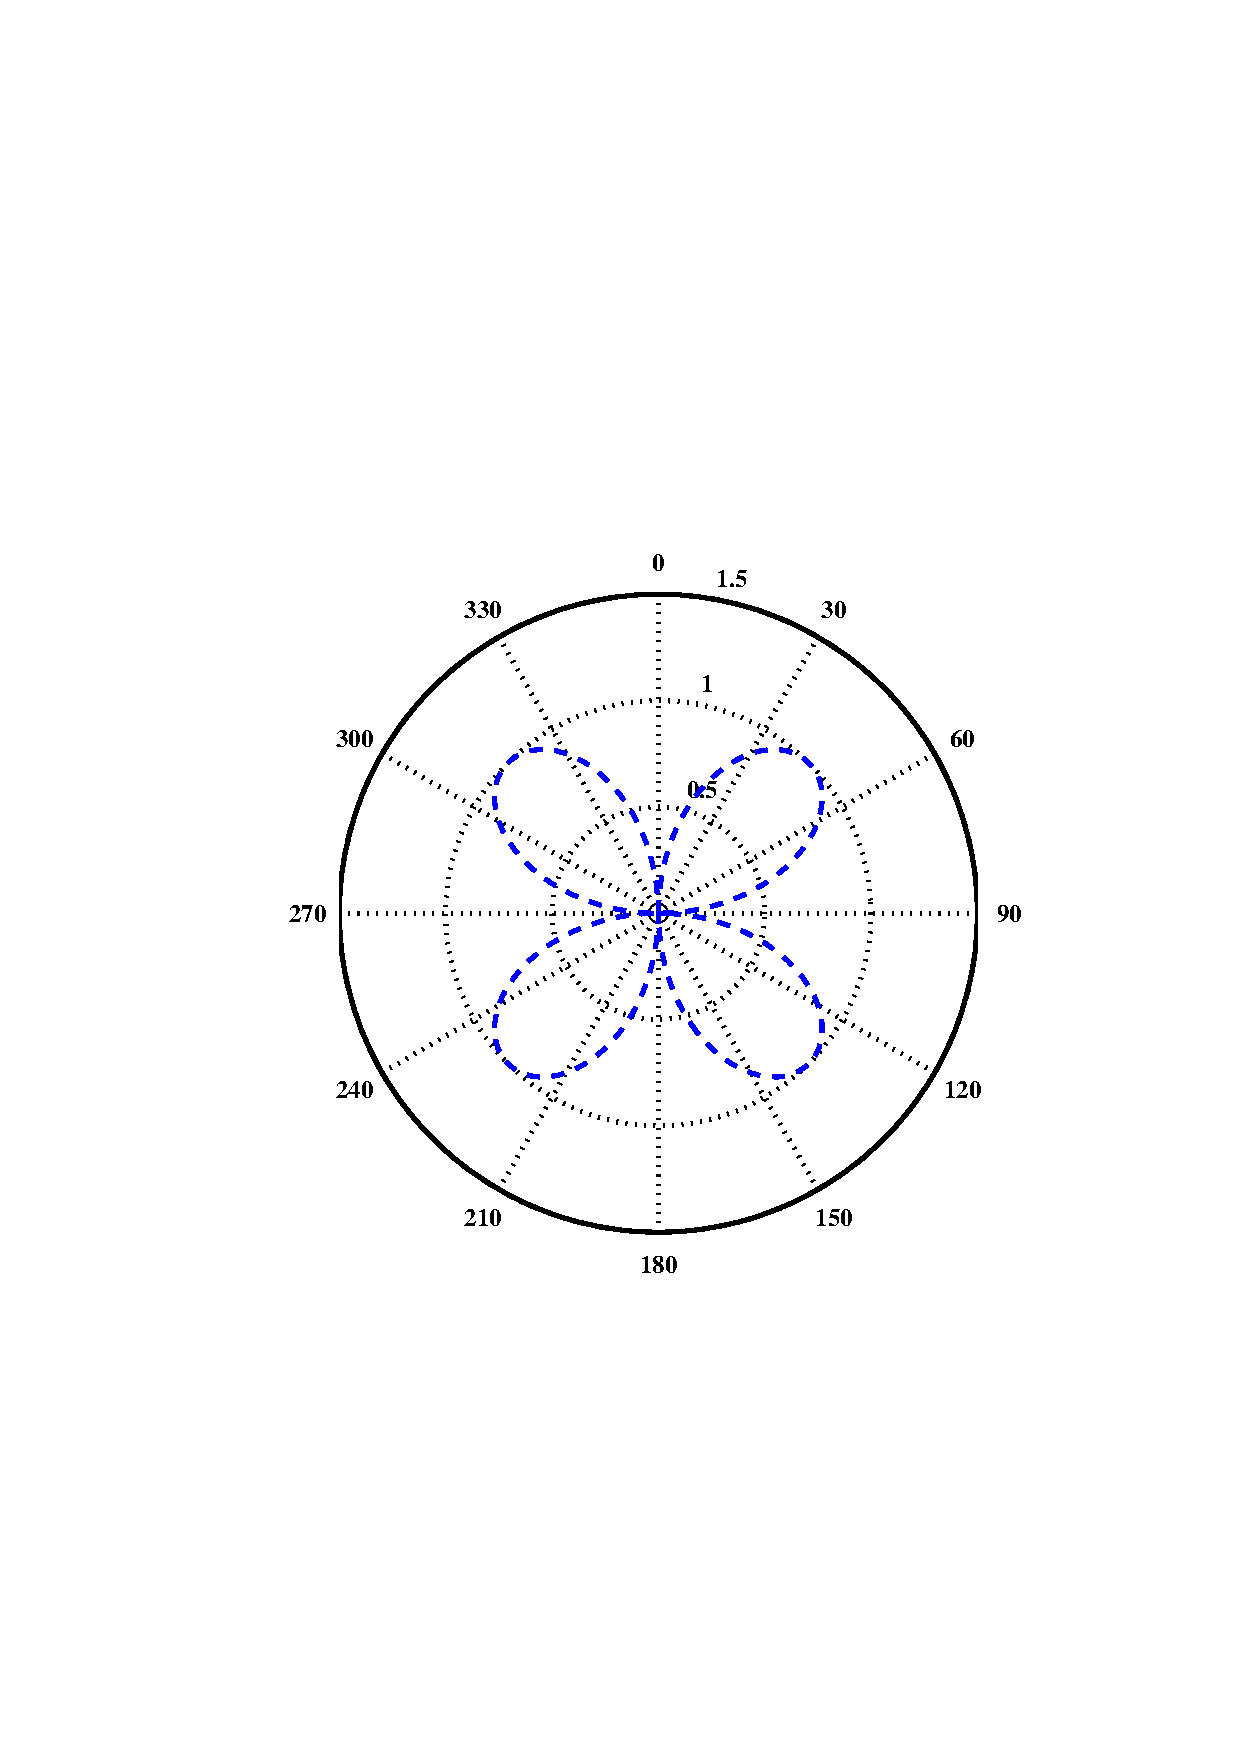
\includegraphics[width=5cm]{radiationpattern/Fig/PS.pdf}}
        \subfloat(c){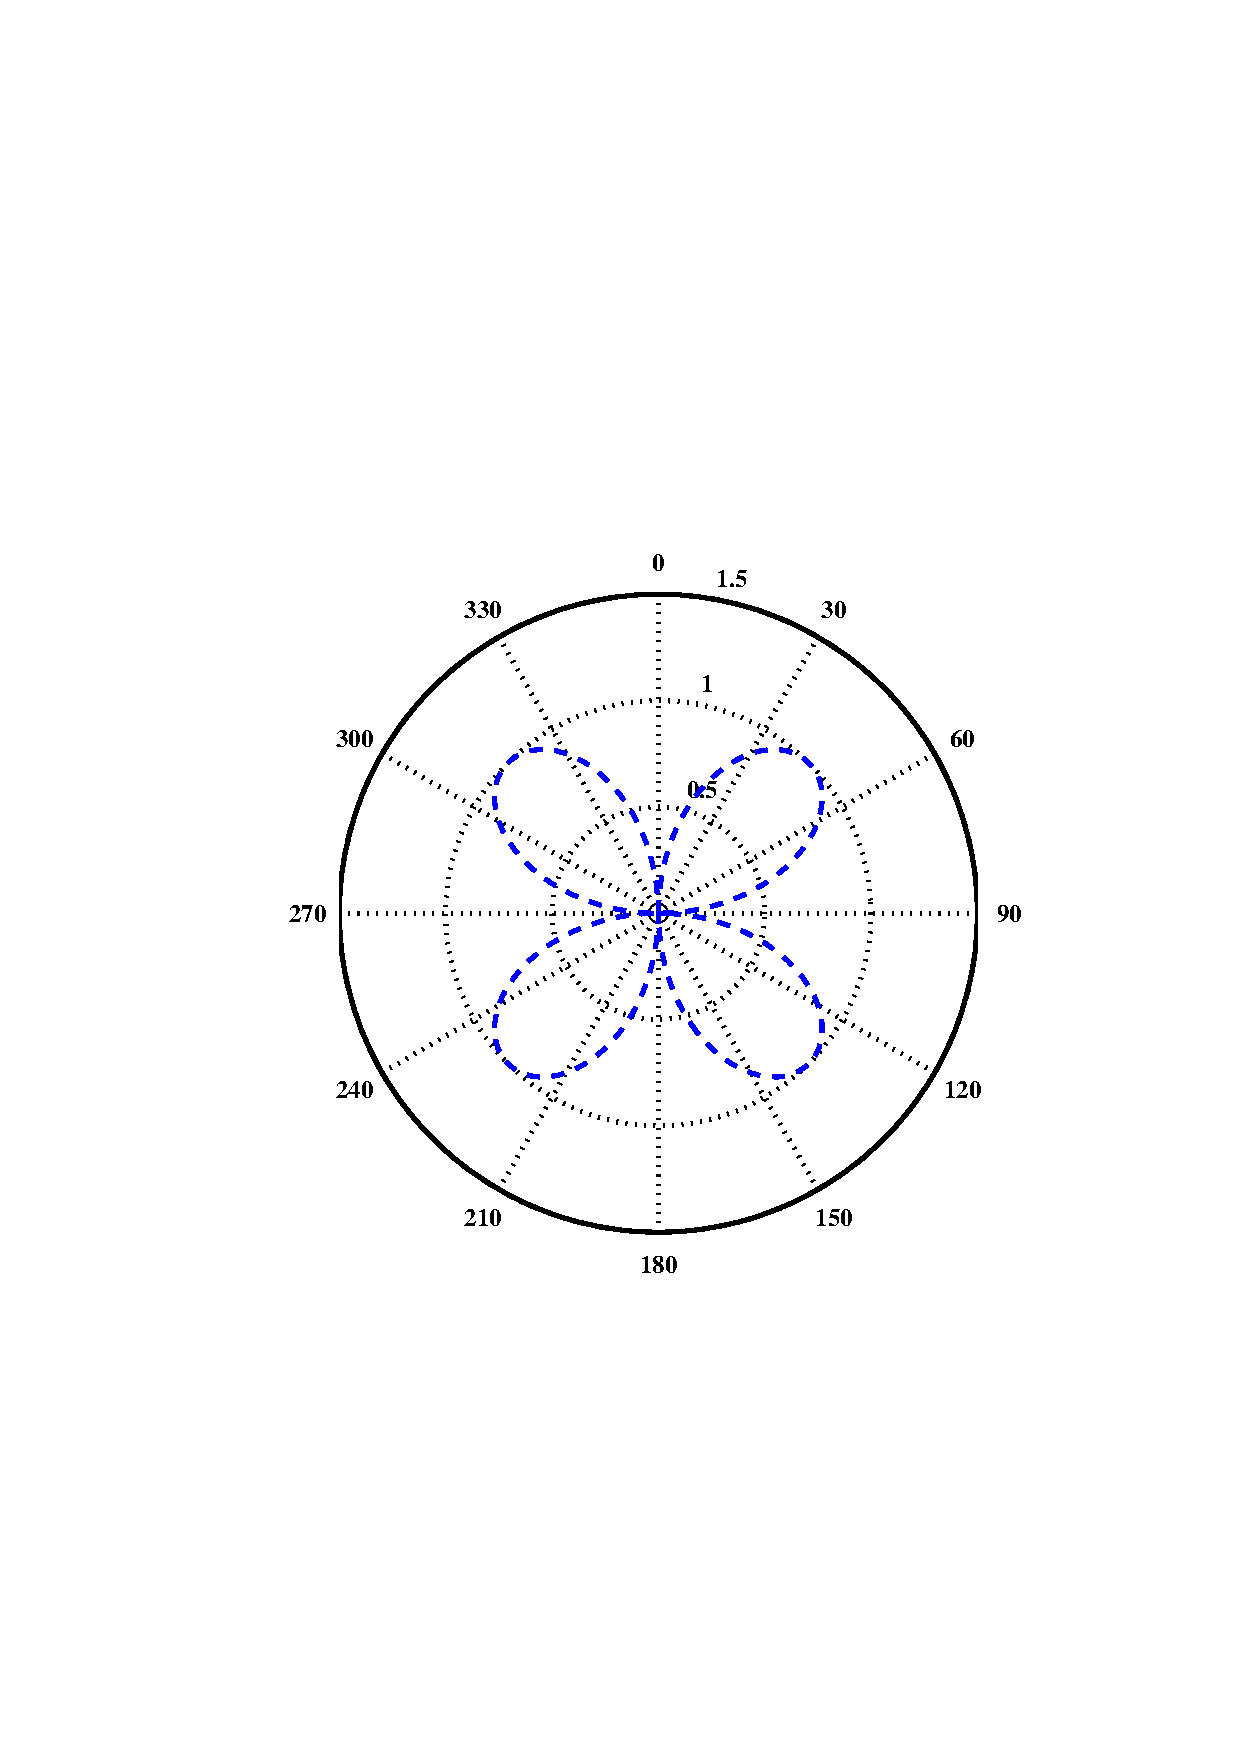
\includegraphics[width=5cm]{radiationpattern/Fig/SP.pdf}}
        \subfloat(d){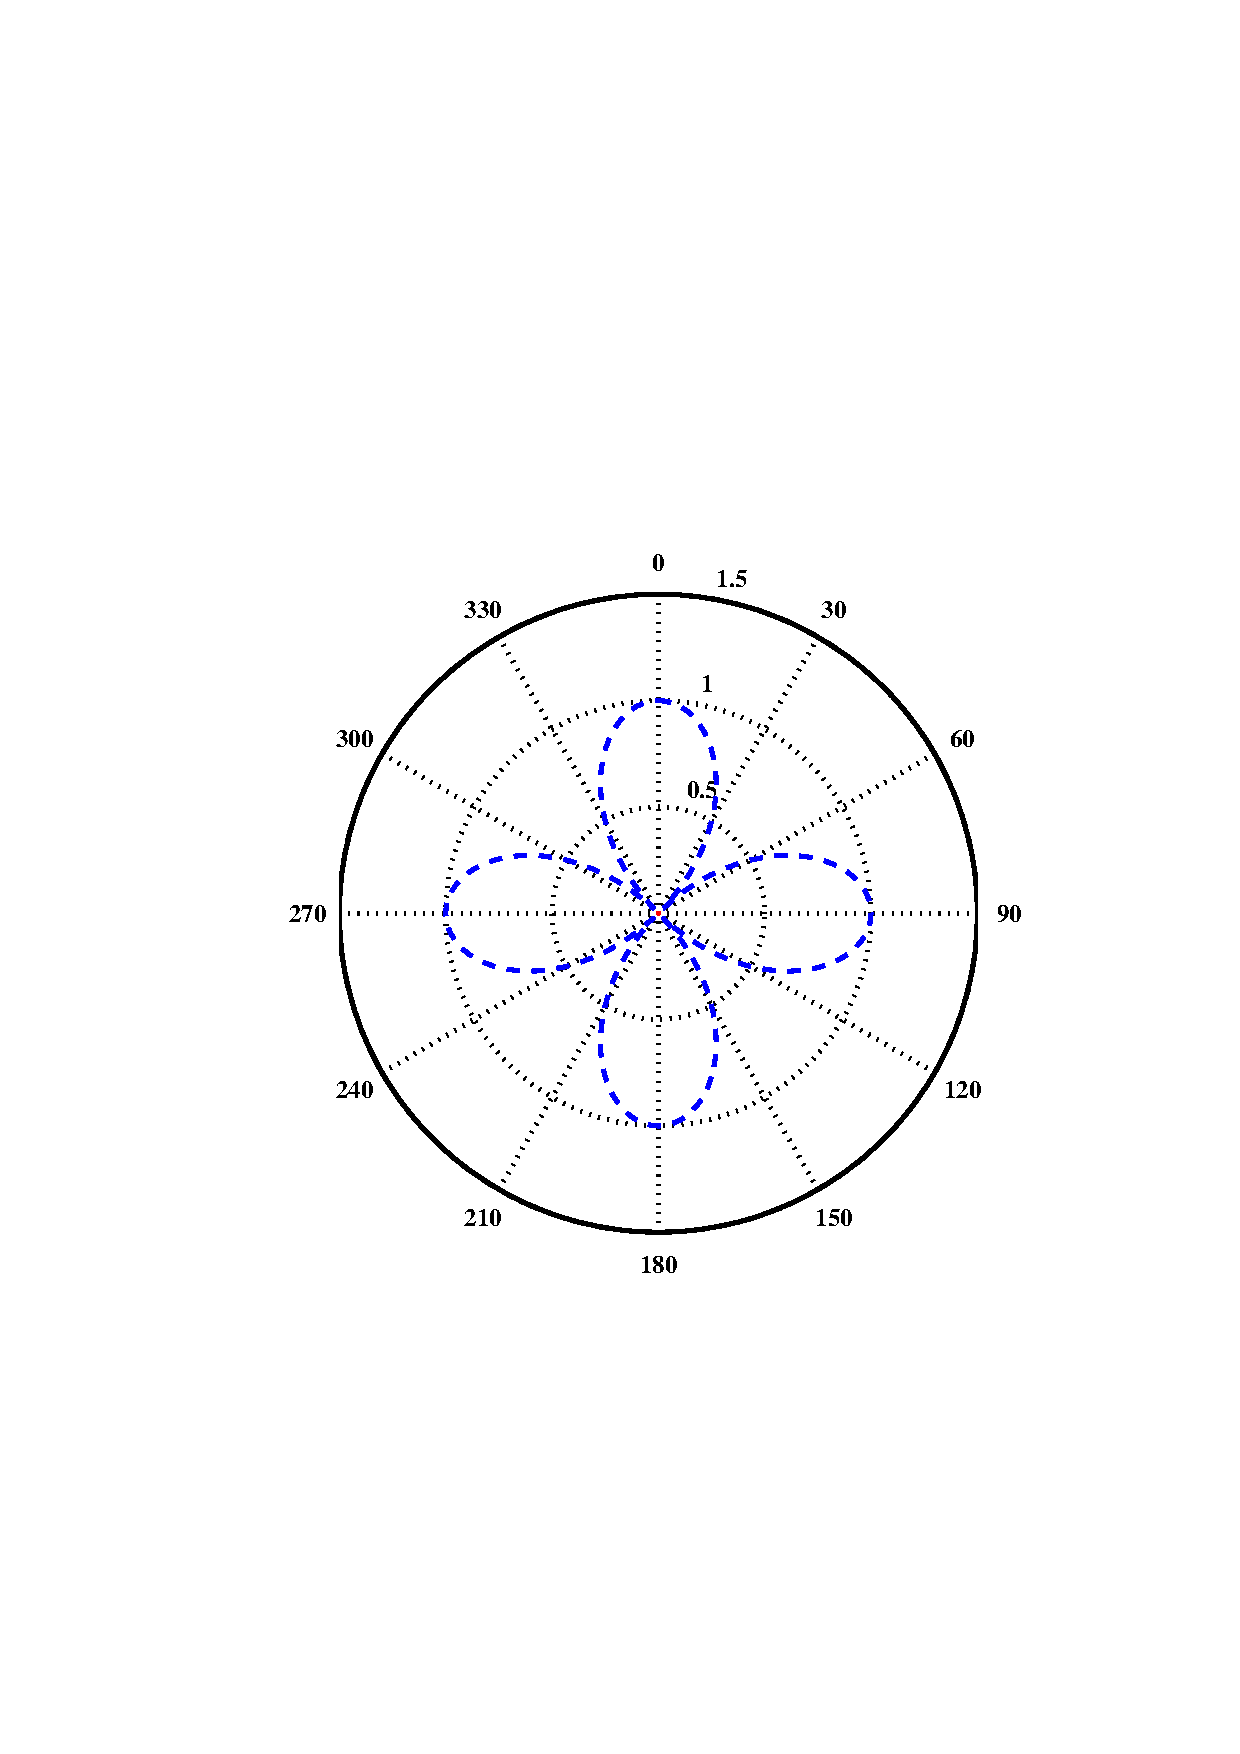
\includegraphics[width=5cm]{radiationpattern/Fig/SS.pdf}}
        \caption{The radiation patterns of $V_p$
        (red) and $V_s$ (blue) perturbations. (a) PP, (b) PS, (c) SP and (d) SS modes.
    }
    \label{fig:radiationpattern} 
    \end{center}
\end{figure*} 

\subsection{弹性波模式解耦}
弹性波波场$\mathbf{u}=(u_x,u_y,u_z)$可以分解成P波波场与S波波场:$\mathbf{u}=\mathbf{u}^P+\mathbf{u}^S$,
其中,$\mathbf{u}^P=(u^P_x,u^P_y,u^P_z)$和$\mathbf{u}^S=(u^S_x,u^S_y,u^S_z)$.
对于各向同性介质而言,该模式解耦方式是不依赖于模型参数的,可在波数域表征为\cite[]{zhang.mcmechan:2010}:
\begin{equation}
        \tilde{\mathbf U}^P=\mathbf k(\mathbf k\cdot \tilde{\mathbf U}), \quad
        \tilde{\mathbf U}^S=-\mathbf 
        k\times(\mathbf k\times \tilde{\mathbf U})
\label{eq:Decomp}
\end{equation}
其中$\mathbf k=(k_x,k_y,k_z)$ 为归一化之后的波矢量,符号$\tilde{}$表示波数域波场。

根据以上推导, 我们将Fr{$\acute{e}$}chet导数分解为不同波模式:
\begin{equation}
        {\mathbf J}_M={\mathbf J}^P_M+{\mathbf J}^S_M,
\label{eq:PropaMDall}
\end{equation}
with
\begin{equation}
        {\mathbf J}^P_M=\mathcal{F}^{-1}(\mathbf k(\mathbf k\cdot \tilde{\mathbf
        J}_M)), \quad
        {\mathbf J}^S_M=\mathcal{F}^{-1}(-\mathbf
                k\times(\mathbf k\times \tilde{\mathbf J}_M)),
\label{eq:PropaMDsplit}
\end{equation}
其中$\mathcal{F}^{-1}$表示从波数域到空间域的反Fourier变换,$\tilde{\mathbf{J}}_M$表示波数域的 Frech{$\acute{e}$}t导数。
这样,方程\eqref{eq:finalMatrixshort}可以按以下方式分裂成两部分:
\begin{equation}
        \mathbf{J}^P\delta\mathbf{m}=\mathbf{\delta u}^P,\quad
        \mathbf{J}^S\delta\mathbf{m}=\mathbf{\delta u}^S,
        \label{eq:UPandUS}
\end{equation}
with
\begin{equation}
        \mathbf{\delta u}=\mathbf{\delta u}^P+\mathbf{\delta u}^S,
        \label{eq:UPS}
\end{equation}
and
\begin{equation}
        \mathbf{J}=\mathbf{J}^P+\mathbf{J}^S,
        \label{eq:JPS}
\end{equation}
其中$\mathbf{J}^P=(\mathbf{J}^P_{V_p}\quad\mathbf{J}^P_{V_s})$和$\mathbf{J}^S=(\mathbf{J}^S_{V_p}\quad\mathbf{J}^S_{V_s})$为大小是$K\times{2L}$的矩阵,分别代表P波或S波分量对应的Frech{$\acute{e}$}t导数(Jacobian矩阵)。
方程\eqref{eq:UPandUS}表示了在模式解耦下的Born近似描述的散射波场。

注意到,次级震源只有在背景波场入射到参数扰动的位置时才会被激发。尽管次级震源(或者说背景场)中会既有P波又有S波,
但是我们发现对于反演来说并不需要严格区分出他们的贡献(原因我们将在讨论部分进行详细阐述)。因此,模式解耦下Jacobian
矩阵满足:
\begin{equation}
        \begin{split} 
        \mathbf{J}^W_M(\mathbf{x}_l,\mathbf{r}_k)=
        \mathbf{T}_M(\mathbf{x}_l):\mathbf{G}'^W(\mathbf{x}_l,\mathbf{r}_k),\quad
        W\in\{P, S\}.
        \end{split}
        \label{eq:EquivFre1}
\end{equation}
该式说明模式解耦算子只作用在了$\mathbf{G}'$上,也即散射Green函数的空间导数。虽然有些学者尝试用”解耦“的方式来
传播P和S波波场\cite{ma.zhu:2003,cheng:2016},但是他们只能在介质参数足够光滑的时候才能获得令人满意的结果\cite[]{brytik:2011,wang.mcmechan:2015b}。
因此,我们并未采用笨拙的传播解耦波场的方法而是采用传播之后用方程\eqref{eq:PropaMDsplit}来进行模式解耦。

\section{反演问题}
方程\eqref{eq:finalMatrixshort}对应的反问题是要找到一个能够解释地震数据的最优模型。该问题的解可以通过求解以下
目标函数的最小值来获得:
\begin{equation}
    E=\frac{1}{2}\delta\mathbf{d}^{\dagger}\delta\mathbf{d},
    \label{eq:misfit}
\end{equation}
其中$\delta\mathbf{d}$ 表示观测数据与模拟数据之间的残差向量,满足$\delta\mathbf{d}=\mathfrak{F}(\mathbf{u}_{obs}-\mathbf{u}_{cal})$,
这里$\mathfrak{F}$ 为位于接收点处的重采样函数,上标$\dagger$表示共轭转置算子。求解该目标函数最小值的标准策略是
采用梯度类或者基于Hessian矩阵的最优化算法。可以通过Jacobian矩阵来求取梯度:
\begin{equation}
        \mathbf{g}=
        \begin{pmatrix}
                \mathbf{g}_{V_p}\\
                \mathbf{g}_{V_s}
        \end{pmatrix}
        =\mathfrak{R}\begin{pmatrix}
                \mathbf{J}^{\dagger}_{V_p}\delta \mathbf{d}\\
                \mathbf{J}^{\dagger}_{V_s}\delta \mathbf{d}
        \end{pmatrix},
        \label{eq:MatrixGra1}
\end{equation}
其中$\mathfrak{R}$表示只取结果的实部。为获得模型更新,梯度导引类方法利用$\mathbf{g}$,而Hessian类方法则利用了
梯度和Hessian矩阵的信息。Hessian类算法能保证四阶的收敛性但即使是声波FWI也要花费庞大的计算与存储代价。
为了在效率与精度之间寻求平衡,我们通常会采用梯度类的方法迭代地求解方程\eqref{eq:misfit},也即:
\begin{equation}
        \mathbf{m}_{k+1}=\mathbf{m}_{k}-\alpha_k \mathbf{g}_k,
        \label{eq:Gradientmethod}
\end{equation}
其中$\mathbf{m}$是模型参数向量,$k$是迭代次数,$\alpha_k$和$\mathbf{g}_k$则分别是第$k$迭代的步长与梯度。
常规的EFWI需要非常多的迭代次数,因此良好的梯度预条件能够加速收敛。

方程\eqref{eq:MatrixGra1}中的梯度并没有内在的机制来判断数据残差的中的变化是来自$\delta V_p$还是来自$\delta V_s$。
我们将方程\eqref{eq:MatrixGra1}分裂为P波与S波分量对应的两个部分:
\begin{equation}
        \begin{pmatrix}
                \mathbf{g}^P_{V_p}\\
                \mathbf{g}^P_{V_s}
        \end{pmatrix}
        =\mathfrak{R}\begin{pmatrix}
                [\mathbf{J}^P_{V_p}+\mathbf{J}^S_{V_p}]^{\dagger}\delta \mathbf{d}^P\\
                [\mathbf{J}^P_{V_s}+\mathbf{J}^S_{V_s}]^{\dagger}\delta \mathbf{d}^P
        \end{pmatrix},
        \label{eq:DEMatrixGraP}
\end{equation}
and
\begin{equation}
        \begin{pmatrix}
                \mathbf{g}^S_{V_p}\\
                \mathbf{g}^S_{V_s}
        \end{pmatrix}
        =\mathfrak{R}\begin{pmatrix}
                [\mathbf{J}^P_{V_p}+\mathbf{J}^S_{V_p}]^{\dagger}\delta \mathbf{d}^S\\
                [\mathbf{J}^P_{V_s}+\mathbf{J}^S_{V_s}]^{\dagger}\delta \mathbf{d}^S
        \end{pmatrix},
        \label{eq:DEMatrixGraS}
\end{equation}
其中,$\mathbf{g}^W_M$为特定波模式(W)的数据残差对应的某一物理参数(M)的梯度。
由于在地面进行P/S数据的分离非常具有挑战,因此数据残差的的分解也会变得非常困难,尤其是在近地表介质非均匀且(或者)
边界条件不完整的情况下。因此需要采取策略来回避多分量地震记录的地面分解。
\begin{figure*}
    \begin{center}
        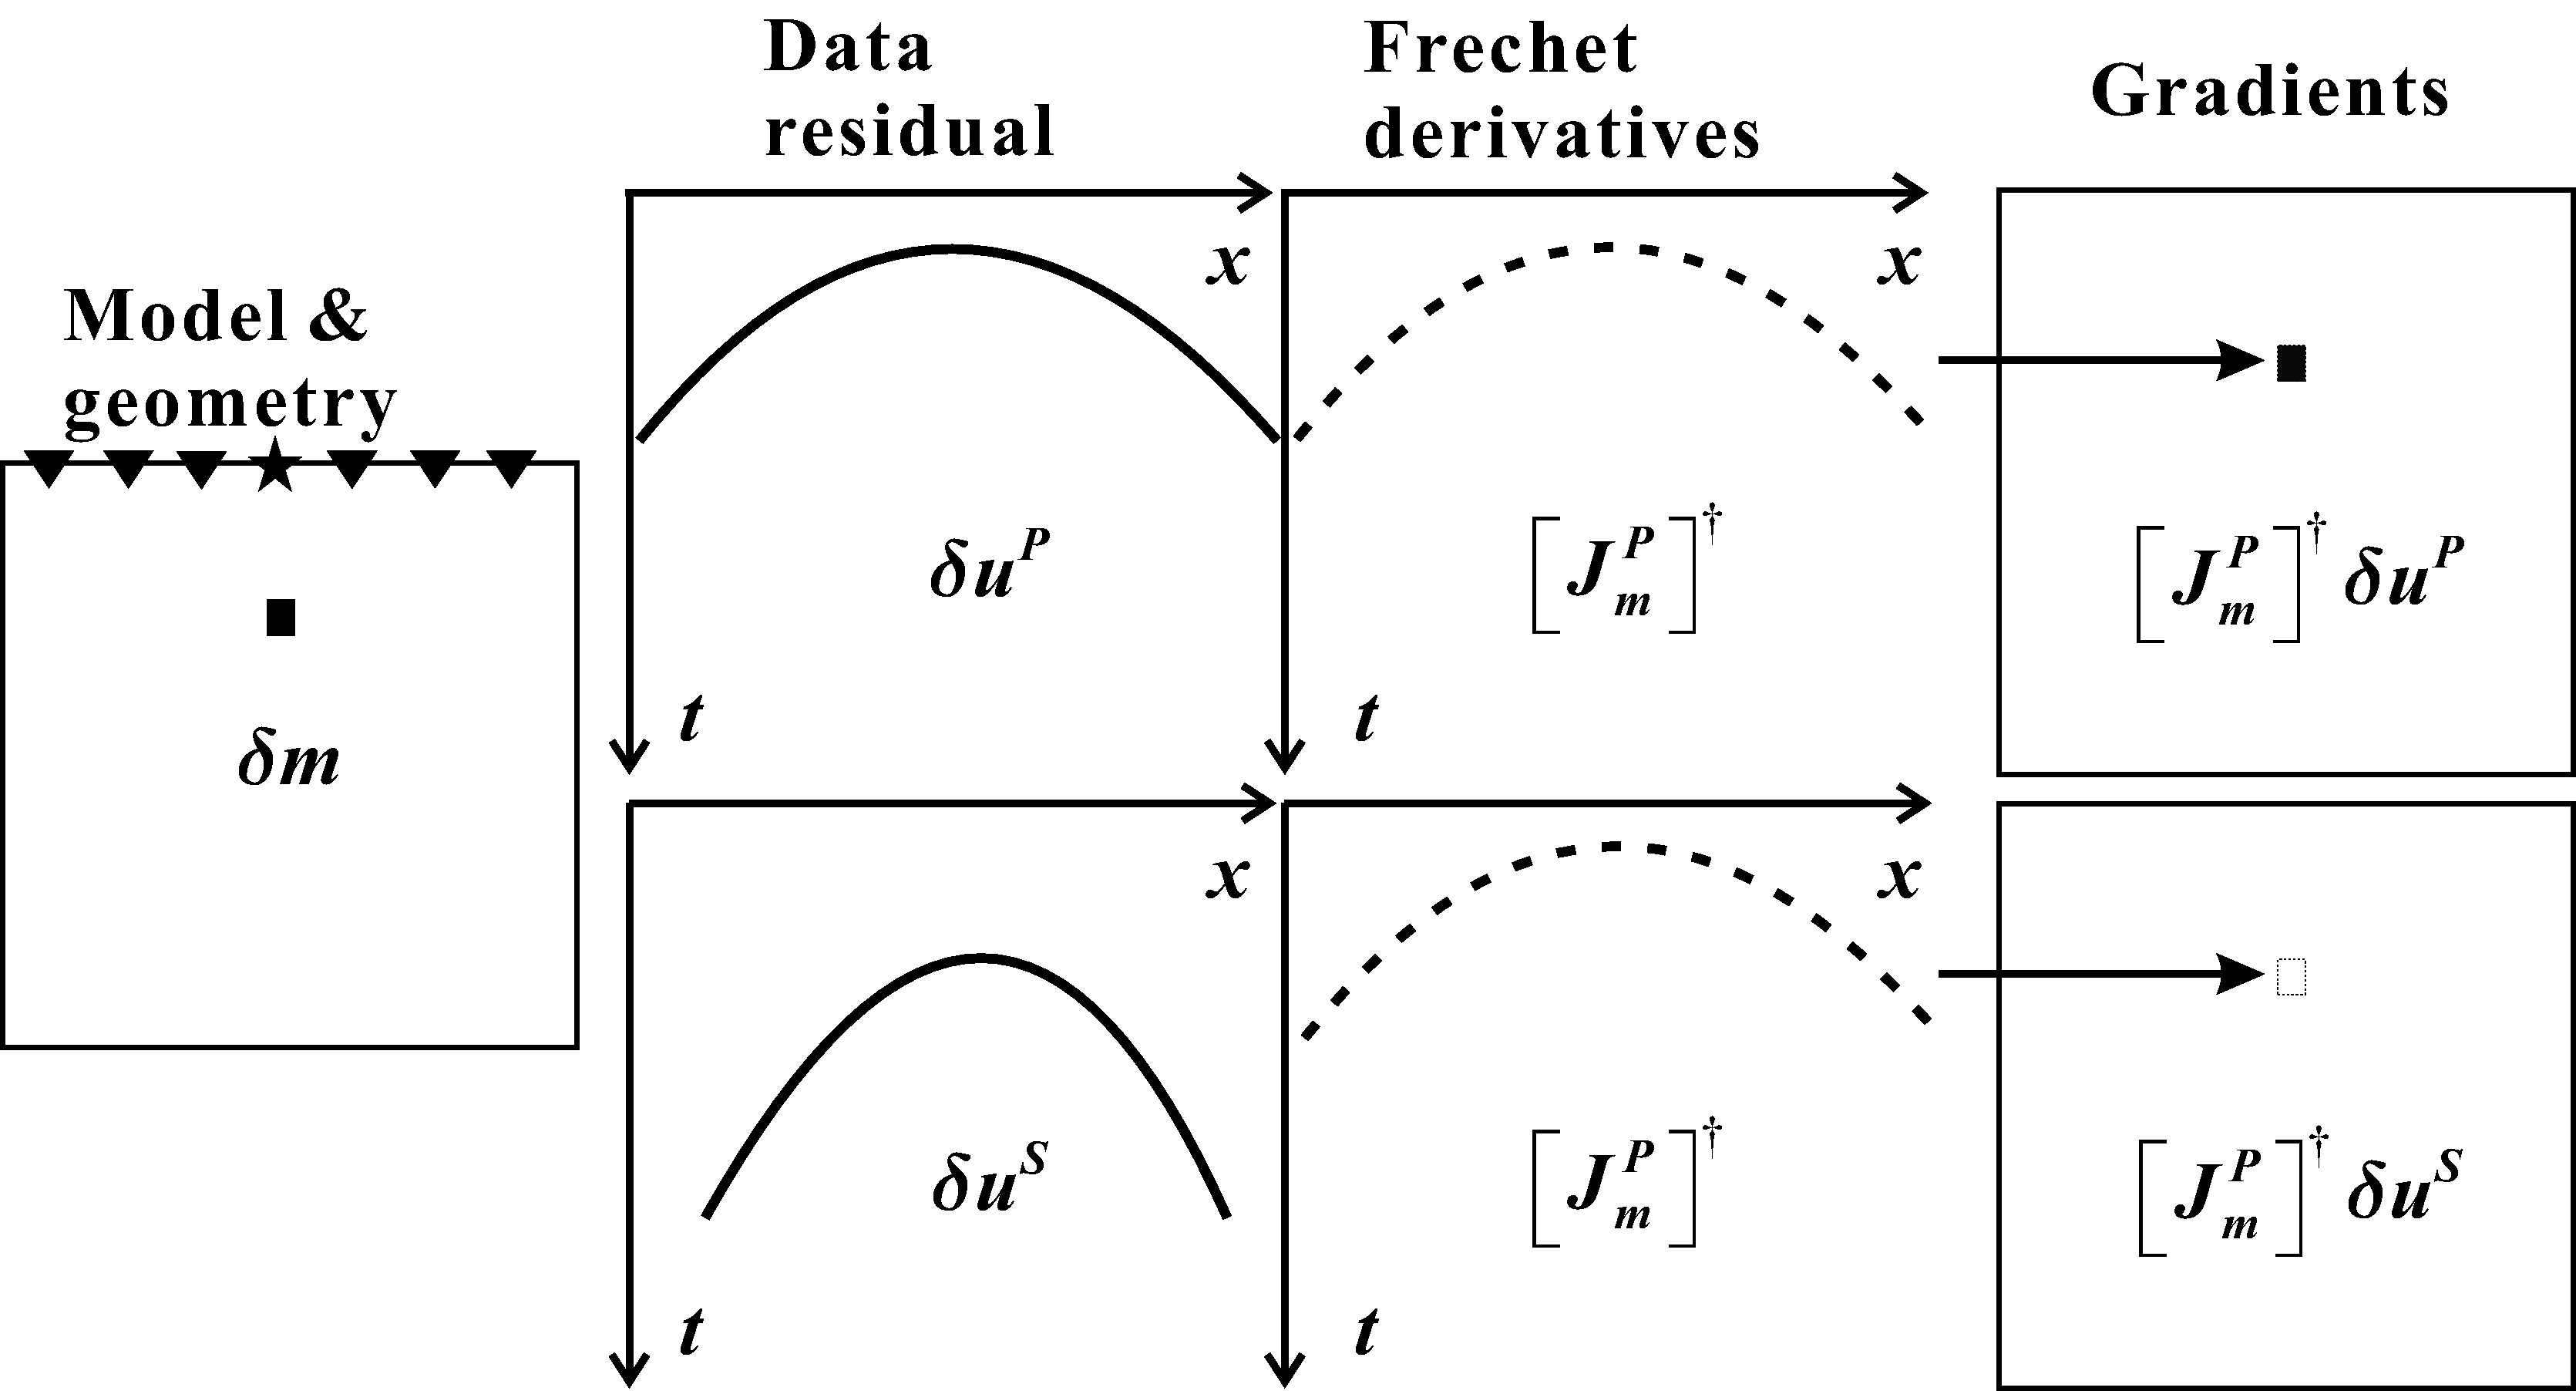
\includegraphics[width=10cm]{finalMarmousiII/Fig/zerolagLAST1.pdf}
        \caption{
Schematic illustration of gradient calculation through zero-lag correlation
 between the partial derivative wavefields
and the residual seismogram.
Only a point perturbation is given in the background media for illustration.
    }
    \label{fig:crossterm}
    \end{center}
\end{figure*}

FWI梯度可看作是偏导数波场与数据残差在时间域的零延迟互相关\cite[]{pratt1998gauss}。如图\ref{fig:crossterm}所示,
假设背景介质中有一个点扰动,数据残差为观测数据与模拟数据之间的差值。偏导数波场代表了由于次级源产生的特征性点绕射响应。
一般而言,P波与S波背景速度不同,因而在偏导数波场和地震记录残差中它们的运动学特征也不同(走时和曲率)。
所以,相同波模式之间的零延迟互相关将在梯度计算中占主要能量,而不同波模式之间的互相关则会由于非同相的干涉被基本消除掉。
因此,我们会有以下的交叉项近似:
\begin{equation}
        \begin{split}
                [\mathbf{J}_{V_p}^{S}]^{\dagger}\delta \mathbf{d}^P\approx\mathbf{0},\\
                [\mathbf{J}_{V_s}^{S}]^{\dagger}\delta \mathbf{d}^P\approx\mathbf{0},\\
                [\mathbf{J}_{V_p}^{P}]^{\dagger}\delta \mathbf{d}^S\approx\mathbf{0},\\
                [\mathbf{J}_{V_s}^{P}]^{\dagger}\delta \mathbf{d}^S\approx\mathbf{0},
        \end{split}
        \label{eq:crossterms}
\end{equation}
其中$\mathbf{0}$为空矩阵。
此外,散射模式说明P波速度的扰动不会产生S波散射,所以我们也有:
\begin{equation}
\mathbf{J}^S_{V_p}=\mathbf{0}.
\label{eq:Jsvp}
\end{equation}
从而有:
\begin{equation}
        \begin{split}
[\mathbf{J}^S_{V_p}]^{\dagger}\delta \mathbf{d}^P=\mathbf{0}, \\
[\mathbf{J}^S_{V_p}]^{\dagger}\delta \mathbf{d}^S=\mathbf{0}.
        \end{split}
\label{eq:Jsvp1}
\end{equation}
\subsection{利用模式解耦对梯度预条件}
利用方程\eqref{eq:crossterms}和\eqref{eq:Jsvp1},我们可以获得以下近似:
\begin{equation}
        \mathbf{J}^{\dagger}_{V_p}\delta \mathbf{d}^P\approx
        [\mathbf{J}^P_{V_p}]^{\dagger}\delta \mathbf{d},\quad
        \mathbf{J}^{\dagger}_{V_s}\delta \mathbf{d}^S\approx
        [\mathbf{J}^S_{V_s}]^{\dagger}\delta \mathbf{d}.
        \label{eq:crossterm}
\end{equation}
因此,基于模式解耦的梯度可以表示为:
\begin{equation}
        \begin{pmatrix}
                \mathbf{g}^P_{V_p}\\
                \mathbf{g}^P_{V_s}
        \end{pmatrix}
        \approx\mathfrak{R}\begin{pmatrix}
                [\mathbf{J}_{V_p}^{P}]^{\dagger}\delta \mathbf{d}\\
                [\mathbf{J}_{V_s}^{P}]^{\dagger}\delta \mathbf{d}
        \end{pmatrix},
        \label{eq:MatrixGraP}
\end{equation}
and
\begin{equation}
        \begin{pmatrix}
                \mathbf{g}^S_{V_p}\\ 
                \mathbf{g}^S_{V_s}
        \end{pmatrix}
        \approx\mathfrak{R}\begin{pmatrix}
                \mathbf{0}\\ 
                [\mathbf{J}^S_{V_s}]^{\dagger}\delta \mathbf{d}
        \end{pmatrix}.
        \label{eq:MatrixGraS}
\end{equation}
上述方程表明在梯度计算中通过Fr{$\acute{e}$}chet导数的解耦来代替数据残差的解耦。

进一步而言,由于串扰效应主要体现在P波数据中,因此我们舍弃梯度中的$\mathbf{g}_{V_s}^P$项来降低参数耦合效应。
所以我们分别选取解耦后的P波与S波Fr{$\acute{e}$}chet导数来构建$V_p$和$V_s$预条件之后的梯度,也即:
\begin{equation}
        \begin{pmatrix}
                \hat{\mathbf{g}}_{V_p}\\
                \hat{\mathbf{g}}_{V_s}
        \end{pmatrix}=
        \begin{pmatrix}
                \mathbf{g}_{V_p}^P\\
                \mathbf{g}_{V_s}^S
        \end{pmatrix}
        \approx 
        \mathfrak{R}\begin{pmatrix}
                [\mathbf{J}^P_{V_p}]^{\dagger} \delta \mathbf{d}\\
                [\mathbf{J}^S_{V_s}]^{\dagger} \delta \mathbf{d}
        \end{pmatrix}.
        \label{eq:MatrixGraMode}
\end{equation}
这里我们用符号$\hat{}$来指示基于模式解耦的预条件梯度。
最终,EFWI问题转化为通过解耦的方式来迭代求解:
\begin{equation}
        \mathbf{m}_{k+1}=\mathbf{m}_{k}-\alpha_k
        \begin{bmatrix}\mathbf{Q}_1\hat{\mathbf{g}}_{V_p}\\\mathbf{Q}_2\hat{\mathbf{g}}_{V_s}\end{bmatrix}_{k},
        \label{eq:Gradientmethod}
\end{equation}
其中,$\mathbf{Q}_1$和$\mathbf{Q}_2$表示预条件算子。步长$\alpha_k$采用抛物线拟合的方式来搜寻\cite[]{vigh20083d}。

\subsection{共轭状态法计算梯度}
显式的计算Fr{$\acute{e}$}chet导数需要进行多达模型网格数量次的正演模拟,这在实际计算中是无法实现\cite[]{virieux2009overview}。
为了避免显式构建Jacobian矩阵,我们采用共轭状态法来计算梯度\cite[]{tromp2005seismic,plessix2006}。利用Green函数的空间互易性,方程\eqref{eq:MatrixGra1}中的原始梯度可以通过正传波场与反传的残差波场之间的时间域
零延迟互相关计算得到:
\begin{equation} 
        \begin{split}
        \mathbf{g}_{V_p}&=-2\rho V_p\int_{0}^{T}\frac{\partial u_i}{\partial
        x_j}\frac{\partial \psi_k}{\partial x_l}
        \delta_{ij}\delta_{kl}dt,\\
        \mathbf{g}_{V_s}&=-2\rho V_s\int_{0}^{T}\frac{\partial u_i}{\partial
        x_j}\frac{\partial \psi_k}{\partial x_l}
        (-2\delta_{ij}\delta_{kl}+\delta_{ik}\delta_{jl}+\delta_{il}\delta_{jk})dt,
        \end{split}
        \label{eq:Gradient_vpvs}
\end{equation}
其中$u_i$是从震源出发的正传波场,$\psi_k$ 是通过数据残差从接收点处反传重建的共轭波场。注意方程\eqref{eq:Gradient_vpvs}
中第一行的算式中自动隐含了正传和共轭波场的散度算子。

从方程\eqref{eq:EquivFre1}可看出,Frech$\acute{e}$t导数的模式解耦等价于施加在散射Green函数上。也说明了,当使用伴随状态法时,
我们只需要解耦伴随波场就可以获得预条件后的梯度,也即:
\begin{equation} 
        \begin{split} 
                \hat{\mathbf{g}}_{V_p}&=-2\rho V_p\int_{0}^{T}\frac{\partial u_i}{\partial
        x_j}\frac{\partial \psi^P_k}{\partial x_l}
        \delta_{ij}\delta_{kl}dt,\\
        &=-2\rho V_p\int_{0}^{T}\frac{\partial u_i}{\partial
        x_j}\frac{\partial \psi_k}{\partial x_l}
        \delta_{ij}\delta_{kl}dt,\\
                \hat{\mathbf{g}}_{V_s}&=-2\rho V_s\int_{0}^{T}\frac{\partial u_i}{\partial
        x_j}\frac{\partial \psi^S_k}{\partial x_l}
        (\delta_{ik}\delta_{jl}+\delta_{il}\delta_{jk})dt,
        \end{split}
        \label{eq:DeGradient_vpvs} 
\end{equation}
其中$\psi^P$和$\psi^S$分别为P波和S波的伴随波场。由于$\mathbf{g}_{V_p}$的计算中隐含了散度算子,总是满足$\hat{\mathbf{g}}_{V_p}=\mathbf{g}_{V_p}$。
对比方程\eqref{eq:Gradient_vpvs},由于S波的散度总是为0,所以在计算预条件后的S波速度梯度时我们舍弃了$-2\delta_{ij}\delta_{kl}$项。
因此,对于P波速度而言,模式解耦已经自动隐含在梯度计算中,但是S波速度的梯度模式解耦预条件需要显式的施加。

解耦伴随波场需要额外的计算量,主要体现在每个时间片中需要两次Fourier变换。为了减少计算量并节省内存消耗,我们
对正传波场与反传波场在时间轴上进行重采样,并且在互相关之前只对反传的伴随波场进行模式解耦。
当更多的多尺度策略考虑进来的时候,也可以对正传波场进行解耦,例如在单级反演中单独的使用S-S或者P-S模式。但是我们并不推荐
这样的策略,我们将在讨论部分进行阐述。
\section{模式解耦降低参数耦合的机制}
	在前一节中我们提出了通过模式解耦来第梯度进行预条件的EFWI方式。然而解决参数解耦问题最直接有效(但也最昂贵)
的方法是考虑Hessian矩阵的优化方法。我们将采用解耦后的
Frech$\acute{e}$t导数来调查Hessian和分辨率矩阵的性质,并且对比高斯牛顿梯度与模式解耦方法的梯度来
分析EFWI中模式解耦降低参数耦合的机制。
\subsection{Hessian矩阵及其不同模式的分量}
多参数的Hessian矩阵是一个具有块状结构的对称方阵,其中非对角块测量了不同物理参数的偏导数波场之间的互相关结果,其作用也
是来处理多参数反演中的参数耦合问题。当反问题为近似线性或者数据残差非常小的时候,全Hessian将约等于近似Hessian
$\mathbf{H}_a$\cite[]{pratt1998gauss}:
\begin{equation}
\mathbf{H}_a =\mathfrak{R}[{\mathbf{J}}^{\dagger}\mathbf{J}]. 
\label{eq:hess}
\end{equation}
考虑到Fr{$\acute{e}$}chet导数的解耦(见方程\ref{eq:JPS}),我们可以将 $\mathbf{H}_a$ 分解为四个分量:
\begin{equation}
\begin{split}
\mathbf{H}_a^{PP}=\mathfrak{R}[{\mathbf{J}^{P}}]^{\dagger}[{\mathbf{J}^{P}}],\\
\mathbf{H}_a^{PS}=\mathfrak{R}[{\mathbf{J}^{P}}]^{\dagger}[{\mathbf{J}^{S}}],\\
\mathbf{H}_a^{SP}=\mathfrak{R}[{\mathbf{J}^{S}}]^{\dagger}[{\mathbf{J}^{P}}],\\
\mathbf{H}_a^{SS}=\mathfrak{R}[{\mathbf{J}^{S}}]^{\dagger}[{\mathbf{J}^{S}}].
\end{split}
\label{eq:hessian_component}
\end{equation}
从应用角度来讲,Hessian矩阵通常是无法计算的。为了调查每个分量各自的贡献,我们在一个网格大小为$30\times30$,
空间采样为5m的模型上数值地计算出Hessian矩阵的各个分量。我们在模型的顶部中央放置一个纯P波震源,接收点分布于四个边界上。
近似Hessian矩阵(Fig. \ref{fig:Hessian})及其分量(Fig. \ref{fig:fourHessian})通过时间域的 Frech{$\acute{e}$}t导数显式求出。近似Hessian矩阵中非对角块中明显的非零元素代表了很强的参数耦合效应。我们可以观察到以下
有用的现象:
首先,交叉项分量,$\mathbf{H}_a^{PS}$ and $\mathbf{H}_a^{SP}$对$\mathbf{H}_a$的贡献可以忽略不计。这是由于相应
的Fr{$\acute{e}$}chet导数因为背景的P波和S波速度不同而不具有相干性。注意到,在这些交叉项分量中会有一些非常小值的非零元素。
这是由于Fr{$\acute{e}$}chet导数中震源附近的大
\begin{equation}
        \mathbf{H}_a\approx
        \mathbf{H}_a^{PP}+
        \mathbf{H}_a^{SS}.
        \label{eq:C3}
\end{equation}
\begin{figure*}
    \begin{center}
        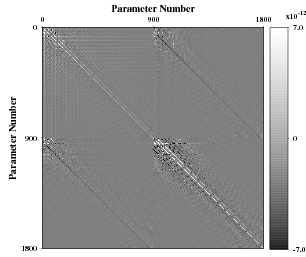
\includegraphics[width=10cm]{ResoOpera/Fig/hessian.pdf}
        \caption{
            The approximate Hessian $\mathbf{H}_a$.
    }
    \label{fig:Hessian} 
    \end{center}
\end{figure*}
\begin{figure*}
    \begin{center}
        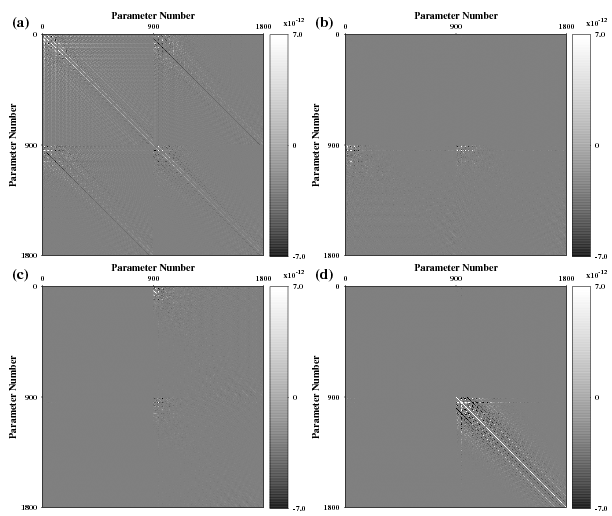
\includegraphics[width=12cm]{ResoOpera/Fig/fourhessian.pdf}
        \caption{
            The four components of the approximate Hessian:
                        (a) $\mathbf{H}_a^{PP}$,
            (b) $\mathbf{H}_a^{PS}$, (c) $\mathbf{H}_a^{SP}$ and (d)$\mathbf{H}_a^{SS}$.
    }
    \label{fig:fourHessian}
    \end{center}
\end{figure*}



其次,$\mathbf{H}_a$的非对角区块几乎与$\mathbf{H}_a^{PP}$一样,并且$\mathbf{H}_a^{SS}$只有右下的对角快是非零的,这是因为$\mathbf{J}^S=(\mathbf{0}\quad\mathbf{J}^S_{V_s})$。这些现象进一步确认了参数耦合主要是来自P波波场而非S波波场。

\subsection{模型分辨率矩阵及其分量}
通过模式解耦的Frech{$\acute{e}$}t导数对Hessian矩阵的定性分析并不足以理解解耦对反演产生作用的机制。为了评估P波与S波数据对
反演的贡献,我们进一步分析模式解耦如何在模型空间影响分辨率矩阵。模型的分辨率矩阵通常采用Hessian矩阵及其逆矩阵来计算得到
\cite[]{menke:1989,snieder1999inverse}。方程\eqref{eq:finalMatrixshort}对应的反问题,我们采用以下公式来更新模型:
\begin{equation}
        \delta \mathbf{\tilde{m}}=-\mathbf{H}^{-1}_a\mathbf{J}^{\dagger}\delta 
        \mathbf{d},
        \label{eq:LeastSol}
\end{equation}
其中$\delta\mathbf{\tilde{m}}$为用全部数据残差估计得到的模型扰动。根据Born近似$\delta\mathbf{d}=\mathfrak{F}{\delta\mathbf{u}}$,
然后将方程\eqref{eq:finalMatrixshort}带入到式\eqref{eq:LeastSol}中,并省略采样函数$\mathfrak{F}$,可以有:
\begin{equation}
	\delta \mathbf{\tilde{m}}=\mathbf{R}\delta \mathbf{m},
	\label{eq:ResoMatr}
\end{equation}
其中$\delta \mathbf{m}$表示真实模型扰动,且模型分辨率矩阵$\mathbf{R}$满足:
\begin{equation}
        \mathbf{R}=-\mathbf{H}^{-g}_a\mathbf{H}_a. 
        \label{eq:ResoOper} 
\end{equation}
注意,由于有限的观测导致近似Hessian总是病态的,因此这里我们采用Hessian的伪逆(广义逆)$\mathbf{H}^{-g}_a$,而不是$\mathbf{H}^{-1}_a$。

\begin{figure*}
    \begin{center}
        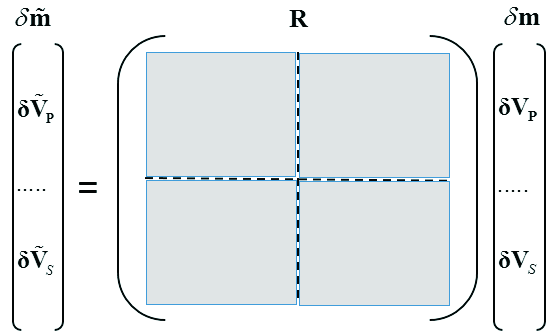
\includegraphics[width=10cm]{ResoOpera/Fig/resolutionmatrix.pdf}
        \caption{
Schematic illustration of the resolution matrix.
The resolution matrix can be divided into four blocks for the inverse problem of two physical parameters.
    }
    \label{fig:IllustrReso}
    \end{center}
\end{figure*}
如图\ref{fig:IllustrReso}所示,模型分辨率矩阵可看作是作用在真实模型上的滤波器。如果观测手段足够好,则分辨率矩阵会是严格的单位矩阵,
也即$\mathbf{R}=\mathbf{I}$,那么模型参数也会是唯一确定的。然而通常情况下$\mathbf{R} \ne \mathbf{I}$,因此对模型的估计将是真实模型参数的加权平均值。
$\mathbf{R}$ 的对角区块隐含了单参数内部间的相互影响及其相应的分辨能力,而非对角区块则表明了不同参数之间的相互作用。如果对角区块上有明显的非零元素分布,
则预示着不可忽视的参数耦合效应。我们如果采用分解后的P波数据,则方程\eqref{eq:LeastSol} 变为:
\begin{equation}
        \delta \mathbf{\tilde{m}}^P=-\mathbf{H}^{-1}_a\mathbf{J}^{\dagger}\delta \mathbf{d}^P,
        \label{eq:LeastSolP}
\end{equation}
其中$\delta \mathbf{\tilde{m}}^P$ 表示P波数据给出的模型估计。同样采用式\eqref{eq:LeastSol}-\eqref{eq:ResoOper}的推导,
我们可以获得P波数据的模型分辨率矩阵:
\begin{equation}
        \mathbf{R}^P=-\mathbf{H}^{-g}_a\mathbf{H}_a^P,
        \label{eq:ResoOperP}
\end{equation}
其中$\mathbf{H}_a^P=\mathbf{J}^{\dagger}\mathbf{J}^P$。类似的,S波的分辨率矩阵为:
\begin{equation}
        \mathbf{R}^S=-\mathbf{H}^{-g}_a\mathbf{H}_a^S,
        \label{eq:ResoOperS}
\end{equation}
且$\mathbf{H}_a^S=\mathbf{J}^{\dagger}\mathbf{J}^S$。容易证明$\mathbf{R}=\mathbf{R}^P+\mathbf{R}^S$。

\begin{figure*}
    \begin{center}
        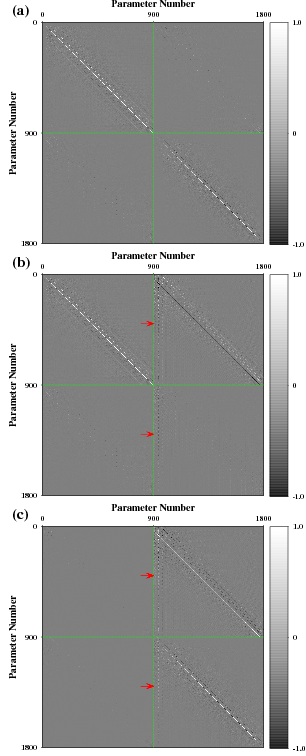
\includegraphics[width=8cm]{ResoOpera/Fig/resolutionoriginal.pdf}
        \caption{
Resolution matrix and its components:
(a) $\mathbf{R}$, (b) $\mathbf{R}^P$ and (c) $\mathbf{R}^S$.
    }
    \label{fig:Resolution}
    \end{center}
\end{figure*}
继续前文所采用的小模型试验,我们可以显式计算出模型分辨率矩阵$\mathbf{R}$,$\mathbf{R}^P$和$\mathbf{R}^S$。
原始分辨率矩阵(图\ref{fig:Resolution}a)为带状对角阵,对角元素为小于1的正值。这说明了近似Hessian的逆可以为$V_p$和$V_s$的反演
提供很好的预条件。P波与S波数据对应的分辨率矩阵(图\ref{fig:Resolution}b和c)展示了一些有趣的现象。例如,$\mathbf{R}^P$和$\mathbf{R}^S$的非零对角块
构成了$\mathbf{R}$。除了一些由于震源附近的干扰而导致的假象,$\mathbf{R}^P$的底部两个区块都为空矩阵。在$\mathbf{R}^P$和$\mathbf{R}^S$的右上区块,其中的元素值
大小相等符号相反,两者相加为零从而能够使得$\mathbf{R}$右上区块为空。这些特征说明,对与线性的反问题(无cycle-skipping),P波与S波都对反演$V_p$有贡献,
而P波对$V_s$的贡献非常弱。常规的梯度法由于只用P波数据来计算$V_p$梯度(见式\ref{eq:Gradient_vpvs}),而这部分P波数据有可能来自$V_s$扰动,从而导致反演受到
参数耦合的影响。此外,单独用S波数据可以很好的分辨$V_s$。模式解耦的预条件方式利用了上述特征,因而其能够压制反演中参数间的耦合。
\subsection{与Gauss-Newton梯度的比较}
GN方法利用近似Hessian的逆对梯度进行预条件来处理参数之间的耦合效应:
\begin{equation}
\delta\tilde{\mathbf{m}} = - \mathbf{H}^{-1}_a\mathbf{g}.
\label{eq:GN}
\end{equation}
假设$\mathbf{H}_a$的伪逆为:
\begin{equation}
        \mathbf{H}^{-g}_a=    
        \begin{bmatrix}
                \mathbf{D}&\mathbf{E} \\
                \mathbf{F}&\mathbf{G}
        \end{bmatrix},
        \label{eq:HessInv}
\end{equation}
则GN方法实际上利用以下公式来更新模型:
\begin{equation}
    \mathbf{{m}}_{k+1}
    =\mathbf{{m}}_{k}-\alpha_k 
    \begin{bmatrix}
        \mathbf{D}\mathbf{g}^P_{V_p} +
        \mathbf{E}\mathbf{g}^P_{V_s}+
        \mathbf{E}\mathbf{g}^S_{V_s}\\
        \mathbf{G}\mathbf{g}^S_{V_s}
    \end{bmatrix}_{k},
    \label{eq:PreGNFi}
\end{equation}
因为
\begin{equation}
        \delta \mathbf{V}^P_s\approx0, \quad \delta \mathbf{V}_s \approx \delta
        \mathbf{V}^S_s=-\mathbf{G}\mathbf{g}^S_{V_s},
        \label{eq:KeyPoint}
\end{equation}
(见附录A)。
\begin{figure*}
    \begin{center}
        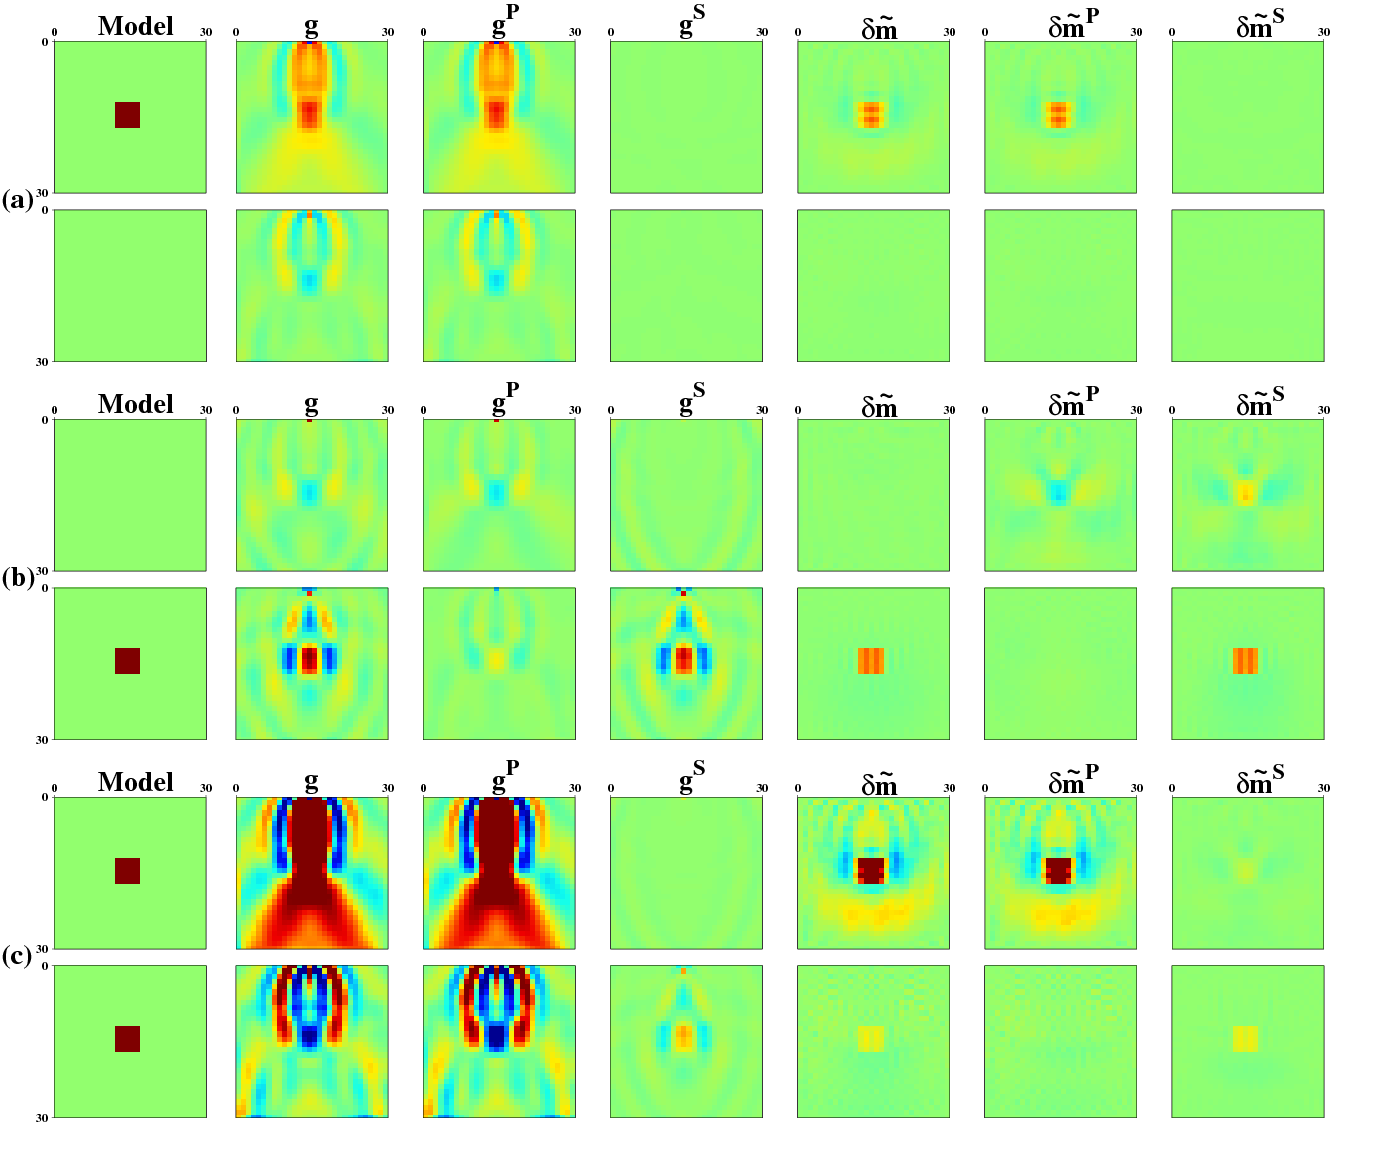
\includegraphics[width=14cm]{Hessiantest/Fig/newepsall.pdf}
        \caption{
    Comparison among the original, GN and MD-based gradients
        of the first iteration:
    (a) $\delta V_p \neq 0$, $\delta V_s=0$; (b) $\delta V_p=0$, $\delta V_s\neq0$; and (c)
    $\delta V_p=10 \delta V_s$.
        Note that there are three panels with two rows and seven columns.
        The first row corresponds to $V_p$, and the second
                corresponds to $V_s$.
    The columns from left to right are the true model $\mathbf{m}=(\mathbf{V}_p,
    \mathbf{V}_s)$;
    the gradients $\mathbf{g}=(\mathbf{g}_{V_p},\mathbf{g}_{V_s})$,
    $\mathbf{g}^P=(\mathbf{g}^P_{V_p},\mathbf{g}^P_{V_s})$,
    $\mathbf{g^S}=(\mathbf{g}^S_{V_p},\mathbf{g}^S_{V_s})$;
    the GN gradients $\delta
    \mathbf{\tilde{m}}=(\delta\mathbf{\tilde{V}}_p,\delta\mathbf{\tilde{V}}_s)$;
        and the preconditioned gradients based on mode decomposition $\delta
        \mathbf{\tilde{m}}^P=(\delta\mathbf{\tilde{V}}^P_p,\delta\mathbf{\tilde{V}}^P_s)$
        and $\delta
        \mathbf{\tilde{m}}^S=(\delta\mathbf{\tilde{V}}^S_p,\delta\mathbf{\tilde{V}}^S_s)$, respectively.
    }
    \label{fig:all}
    \end{center}
\end{figure*}
在图\ref{fig:all}中,我们同样采用前文中小模型实验来比较原始梯度、GN梯度和解耦梯度。
我们在模型中央放置三种不同类型,大小为10$\times$10m的参数扰动组合,分别为:(a) $\delta V_p \neq 0$, $\delta V_s = 0$; (b) $\delta V_p = 0$,
$\delta V_s \neq 0$,和(c) $\delta V_p =10\delta
V_s$。初始模型为均匀的背景速度。在第一组实验中只有P波数据,我们可以看到原始的梯度,$\mathbf{g}_{V_p}$和$\mathbf{g}_{V_s}$中,有非常明显的参数耦合效应。
从图\ref{fig:all}a和b中可以看到,对于物理参数A而言,另一个参数B扰动会产生一个与B扰动方向相反的A的梯度。从图\ref{fig:all}b和c中$\mathbf{g}^{P}_{V_s}$看到,尽管P波数据残差可能携带了$\delta V_s$的信息,
常规梯度类方法用P波数据来反演$V_s$将会受到参数耦合的影响。在第三组实验中,由于参数耦合的影响,$\mathbf{g}^P_{V_s}$甚至提供了错误的更新方向。
而由于S波残差只与$\delta
V_s$有关,因此正如我们所期望的,$\mathbf{g}^S_{V_s}$总是能提供一个正确的更新方向。所以,$\mathbf{g}^P_{V_s}$是梯度参数耦合部分的主要能量。
一般来说,在以P波能量占主导的地震数据中,梯度的参数耦合部分总是带来负面的效应,除非有行之有效的预条件算子,例如图\ref{fig:all}中的GN梯度。

更重要的是,图\ref{fig:all}中最后三列结果在数值上验证了方程\eqref{eq:KeyPoint},同时也展示了模式解耦梯度法与GN方法之间的异同。与常规梯度法不同,
GN方法通过Hessian的逆加权叠加三个解耦之后的梯度,
$\mathbf{g}^P_{V_p}$、$\mathbf{g}^P_{V_s}$和$\mathbf{g}^S_{V_s}$,来获得P波速度梯度的最佳预条件。对于S波速度,GN方法实际上用
$\mathbf{G}$做为算子来对S波数据梯度做预条件处理。而算子$\mathbf{G}$近似等价于$[\mathbf{J}^{S}_{V_s}]^{\dagger}\mathbf{J}^{S}_{V_s}$的伪逆,
见方程\ref{eq:ResoOperS2}。正如方程\eqref{eq:Gradientmethod}所示,模式解耦梯度法也需要进一步的预条件来加速收敛。例如,预条件算子$\mathbf{Q}_2$
只需要达到解决S波的照明补偿以及子波带宽效应即可,也即近似$\mathbf{G}$的效果。因此,对
$V_s$反演,模式解耦梯度法几乎可看作是采用解耦的S波数据进行的单参数反演。所以预条件算子$\mathbf{Q}_2$要更廉价一些,比如利用单参数拟Hessian或者l-BFGS
方法。这种预条件方法为$V_s$反演近似提供了GN梯度同时降低了迭代中的参数耦合,因而其能够在不计算Hessian情况下加速收敛。

\section{数值实验}
本节中,我们用两个理论数据的例子来验证模式解耦EFWI的有效性,同时与常规梯度法的反演结果进行对比。实验中我们采用纯P波震源来合成多分量地震记录。
从较好的初始模型开始,$V_p$和$V_s$将同时被反演。我们在时间域对数据进行低通滤波,然后采用从低频到高频的多尺度策略来避免陷入局部极值。因此,反演
分为四个不同的阶段:0-2Hz,0-4Hz,0-6Hz和0-10Hz。为简单起见,原始梯度法与解耦的梯度法都采用了随深度变化的照明补偿预条件算子\cite[]{kohn:2012}。
\subsection{流体饱和模型}
\begin{figure*}
    \begin{center}
        \subfloat(a){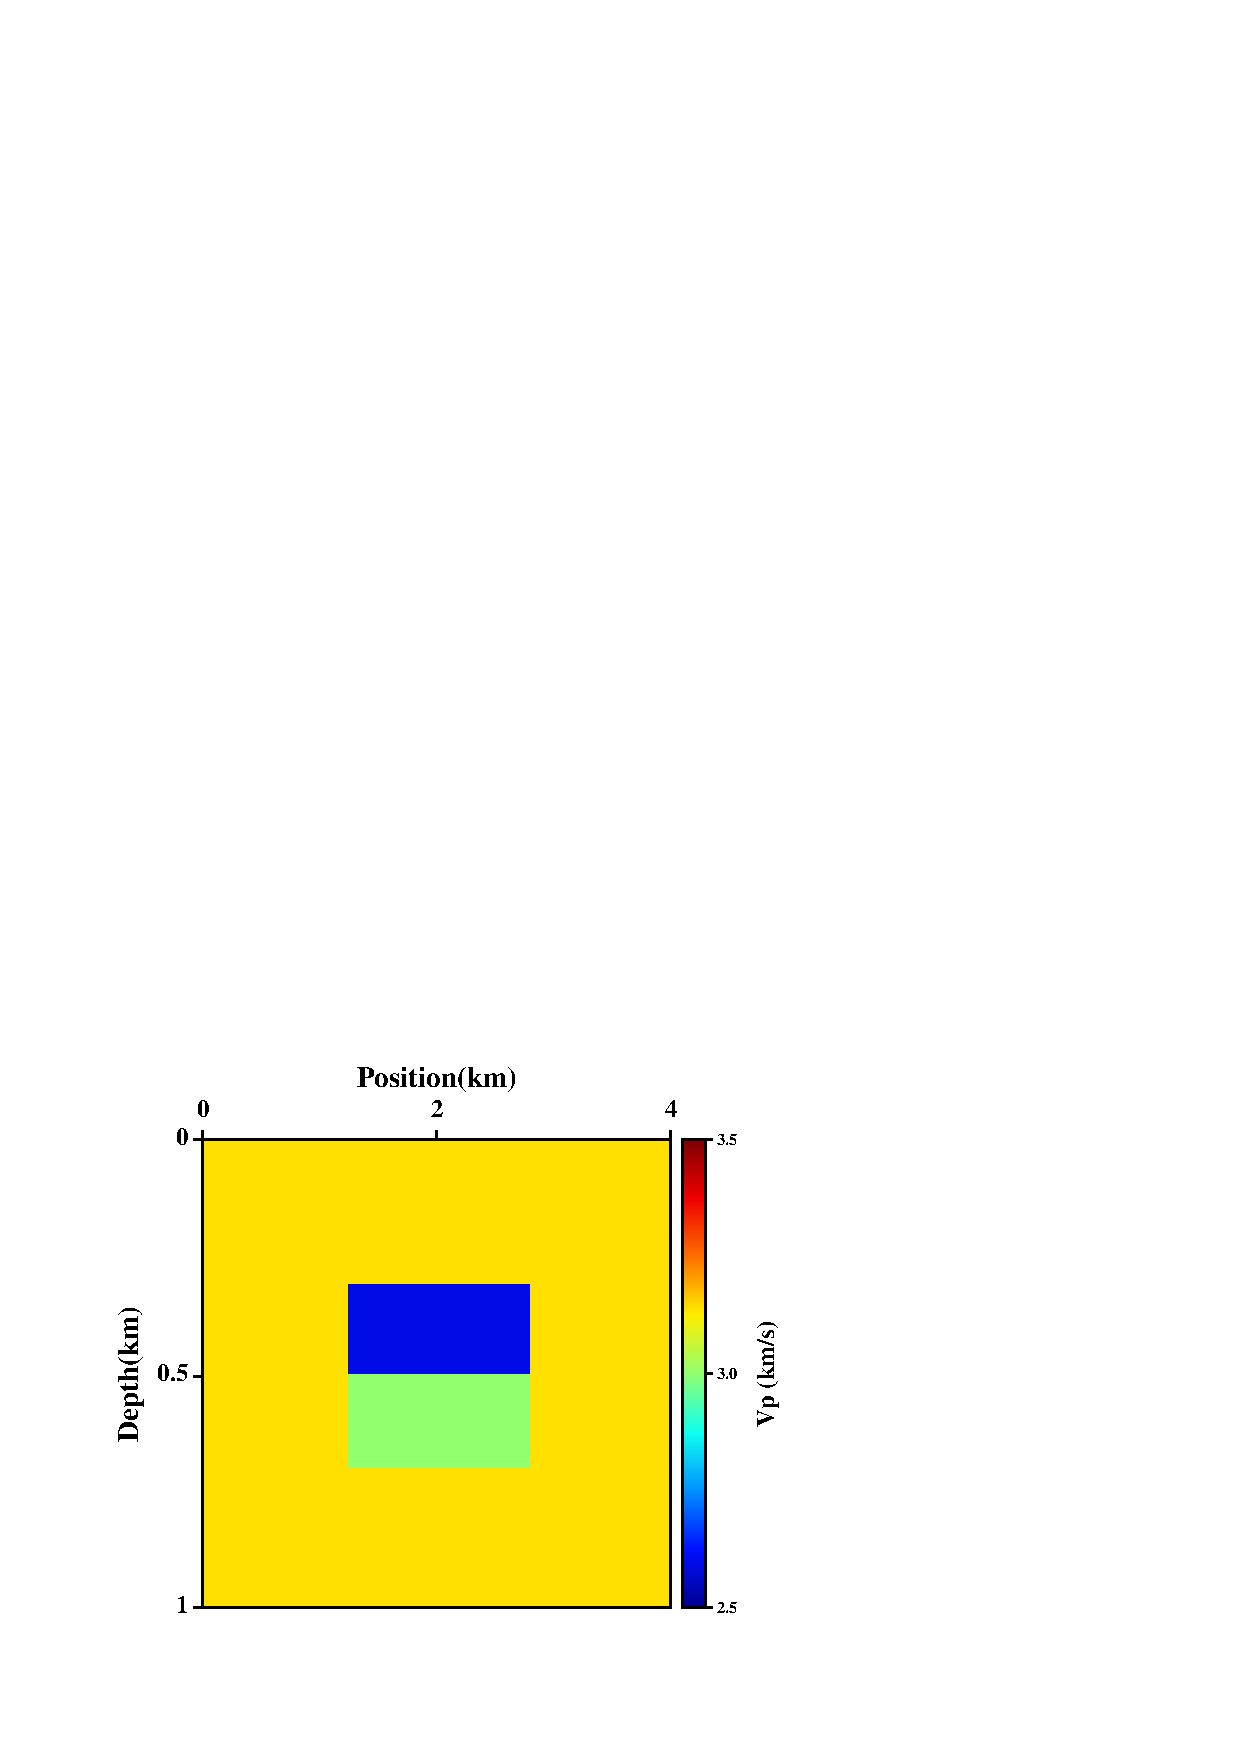
\includegraphics[width=7cm]{smallmodel/Fig/truevp.pdf}}
        \subfloat(b){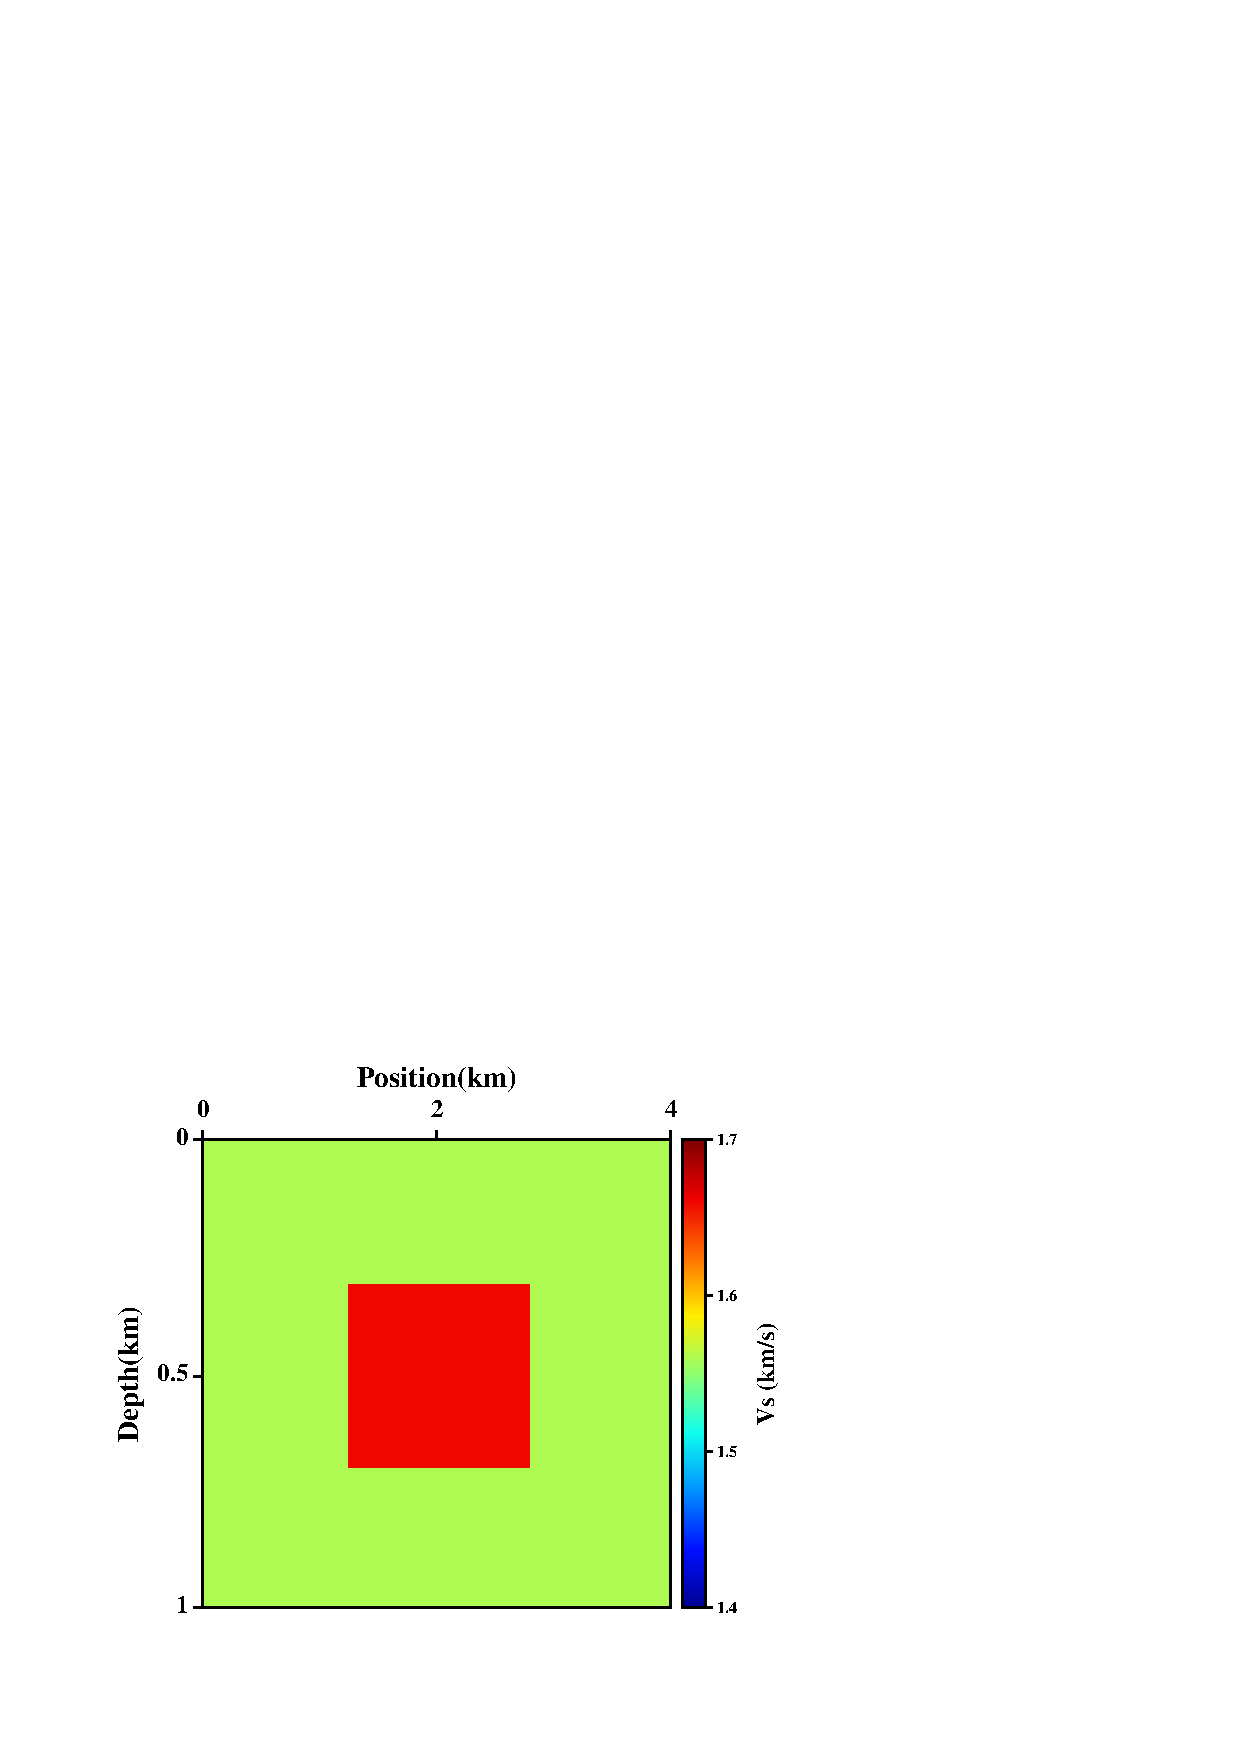
\includegraphics[width=7cm]{smallmodel/Fig/truevs.pdf}}
        \subfloat(c){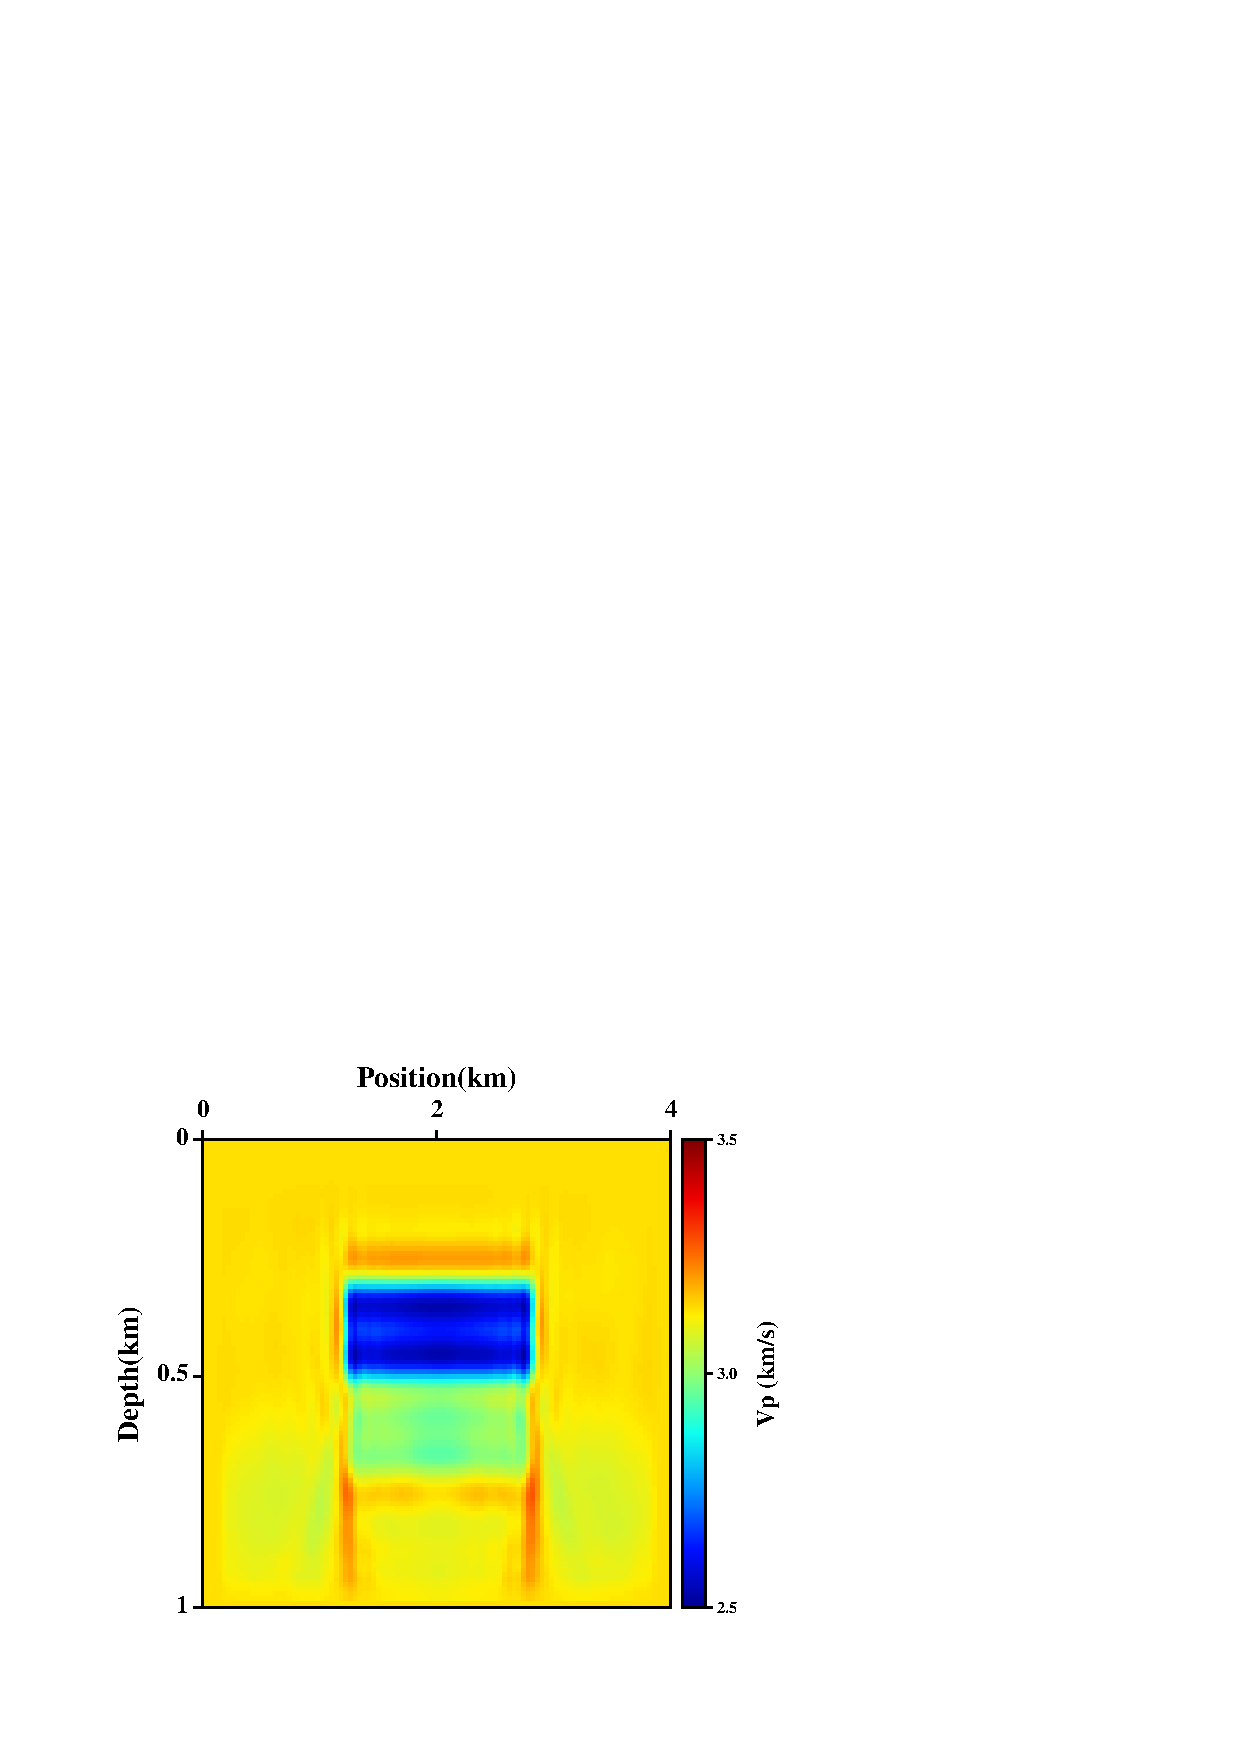
\includegraphics[width=7cm]{smallmodel/Fig/nodecomvp.pdf}}
        \subfloat(d){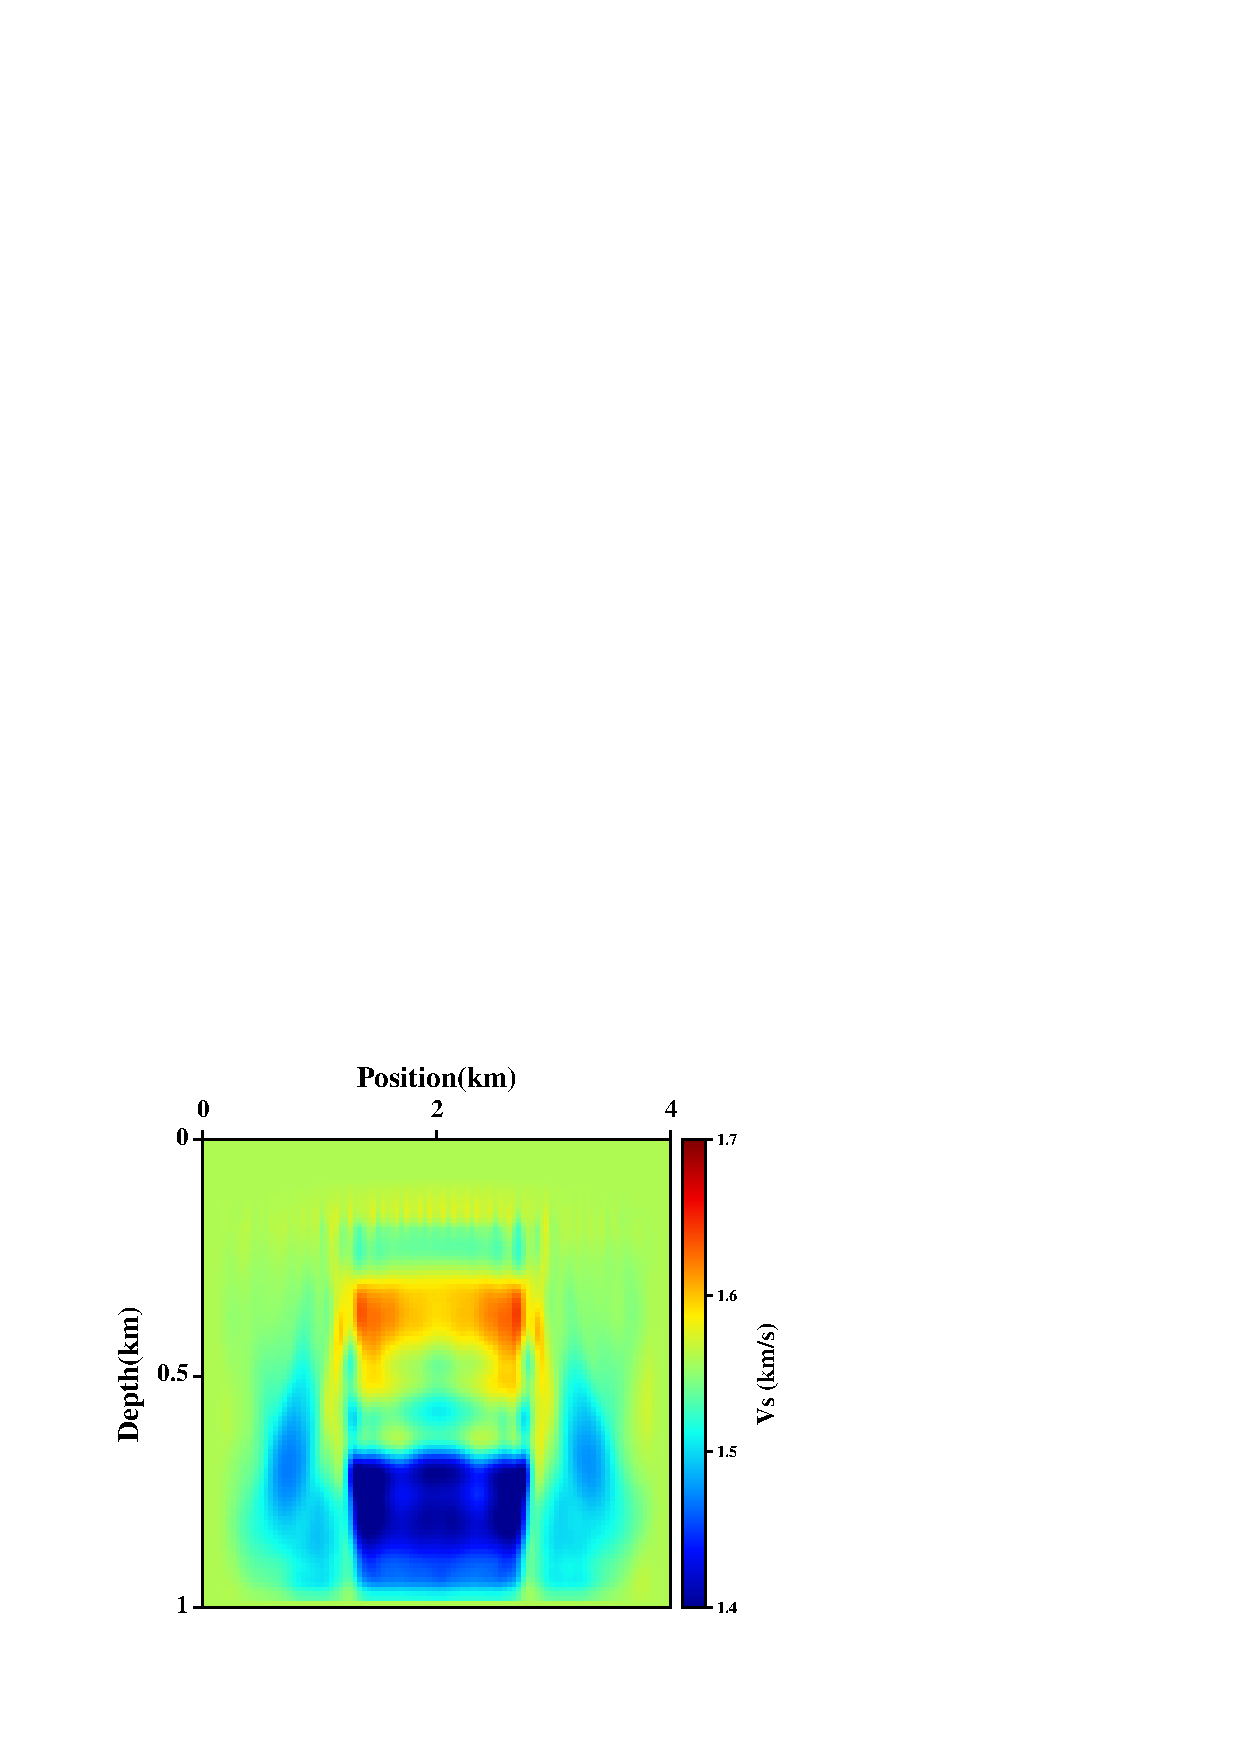
\includegraphics[width=7cm]{smallmodel/Fig/nodecomvs.pdf}}
        \subfloat(e){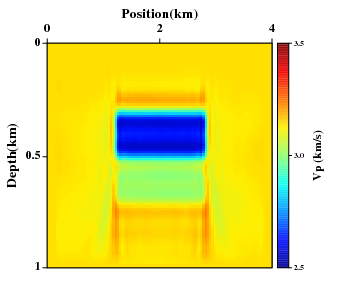
\includegraphics[width=7cm]{smallmodel/Fig/decomvp.pdf}}
        \subfloat(f){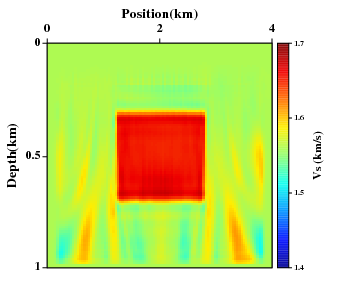
\includegraphics[width=7cm]{smallmodel/Fig/decomvs.pdf}}
        \caption{
            EFWI of a fluid-saturated sandstone model: the true $V_p$ (left) and $V_s$
            (right) models (top),
            and the inverted models using the PCG (mid) and the MD-based (bottom)
            methods, respectively.
    }
    \label{fig:smallmodel}
    \end{center}
\end{figure*}

图\ref{fig:smallmodel}中,我们定义了一个在沙岩背景模型中的流体饱和储层,背景模型参数为$V_p=3.14 km/s$, $V_s=1.56 km/s$以及$\rho=2000 kg/m^{-3}$。储层的上部为气饱和,参数为
$V_p=2.6 km/s$和$V_s=1.66 km/s$,下部为水饱和$V_p=3.0 km/s$和$V_s=1.66 km/s$。
储层的速度值根据沙岩物理模型给出\cite[]{mavko2009rock}。在模型表面,我们合成32炮数据,炮间距为100m,每炮数据为400道记录,道间距为10m。反演从背景模型开始。
每阶段最大迭代次数限制为10次。从反演结果上看,常规EFWI方法能得到可接受的$V_p$模型,而$V_s$反演结果由于很强的参数耦合影响则非常糟糕。
由于在初始阶段,梯度会受到参数耦合的强烈影响,这导致模型中长波长成分的重建受到严重干扰,因此在有限的迭代次数下反演最终收敛到了局部极值中。
但是,因为采用了模式解耦之后的梯度,MD方法最后很好的重建了$V_p$ 和$V_s$模型。
\subsection{Marmousi-II模型}
过去十年间,很多EFWI策略被用在了OBC地震数据中。在低频数据存在的情况下,重建低Poisson值的模型(硬海底)相对比较容易\cite[]{bae:2012}。
然而,软海底环境在现实中更为普遍。这种情况下,有限的PS转换能量,反演中的非线性程度以及参数间的耦合会变得更加严重。为了应对这种更真实的软海底情况,、
如图\ref{fig:MarInitTrue}(a)和(b)所示,我们用Marmousi-II模型中的原始P波与S波速度来测试我们的算法。不同参数间非一致的结构能更明显地表明参数间的耦合。
为了更好的展示MD方法的优势,我们在S波速度模型1.5km深处添加一个高速的薄层。在反演中,我们采用交错网格有限差分来计算正传与共轭波场,空间采样间隔为5m。
记录总时间为8s,时间采样间隔为0.5ms。共有40炮合成数据,炮点深度在20m的水深处,2800个检波点放置于海底来模拟OBC观测。初始模型通过SU软件中的smooth2函数
来平滑真实模型产生,平滑半径为300m。我们采用与前一实验同样的多尺度策略,但是每阶段最大迭代次数扩大为40次。
\begin{figure*}
    \begin{center}
        \subfloat(a){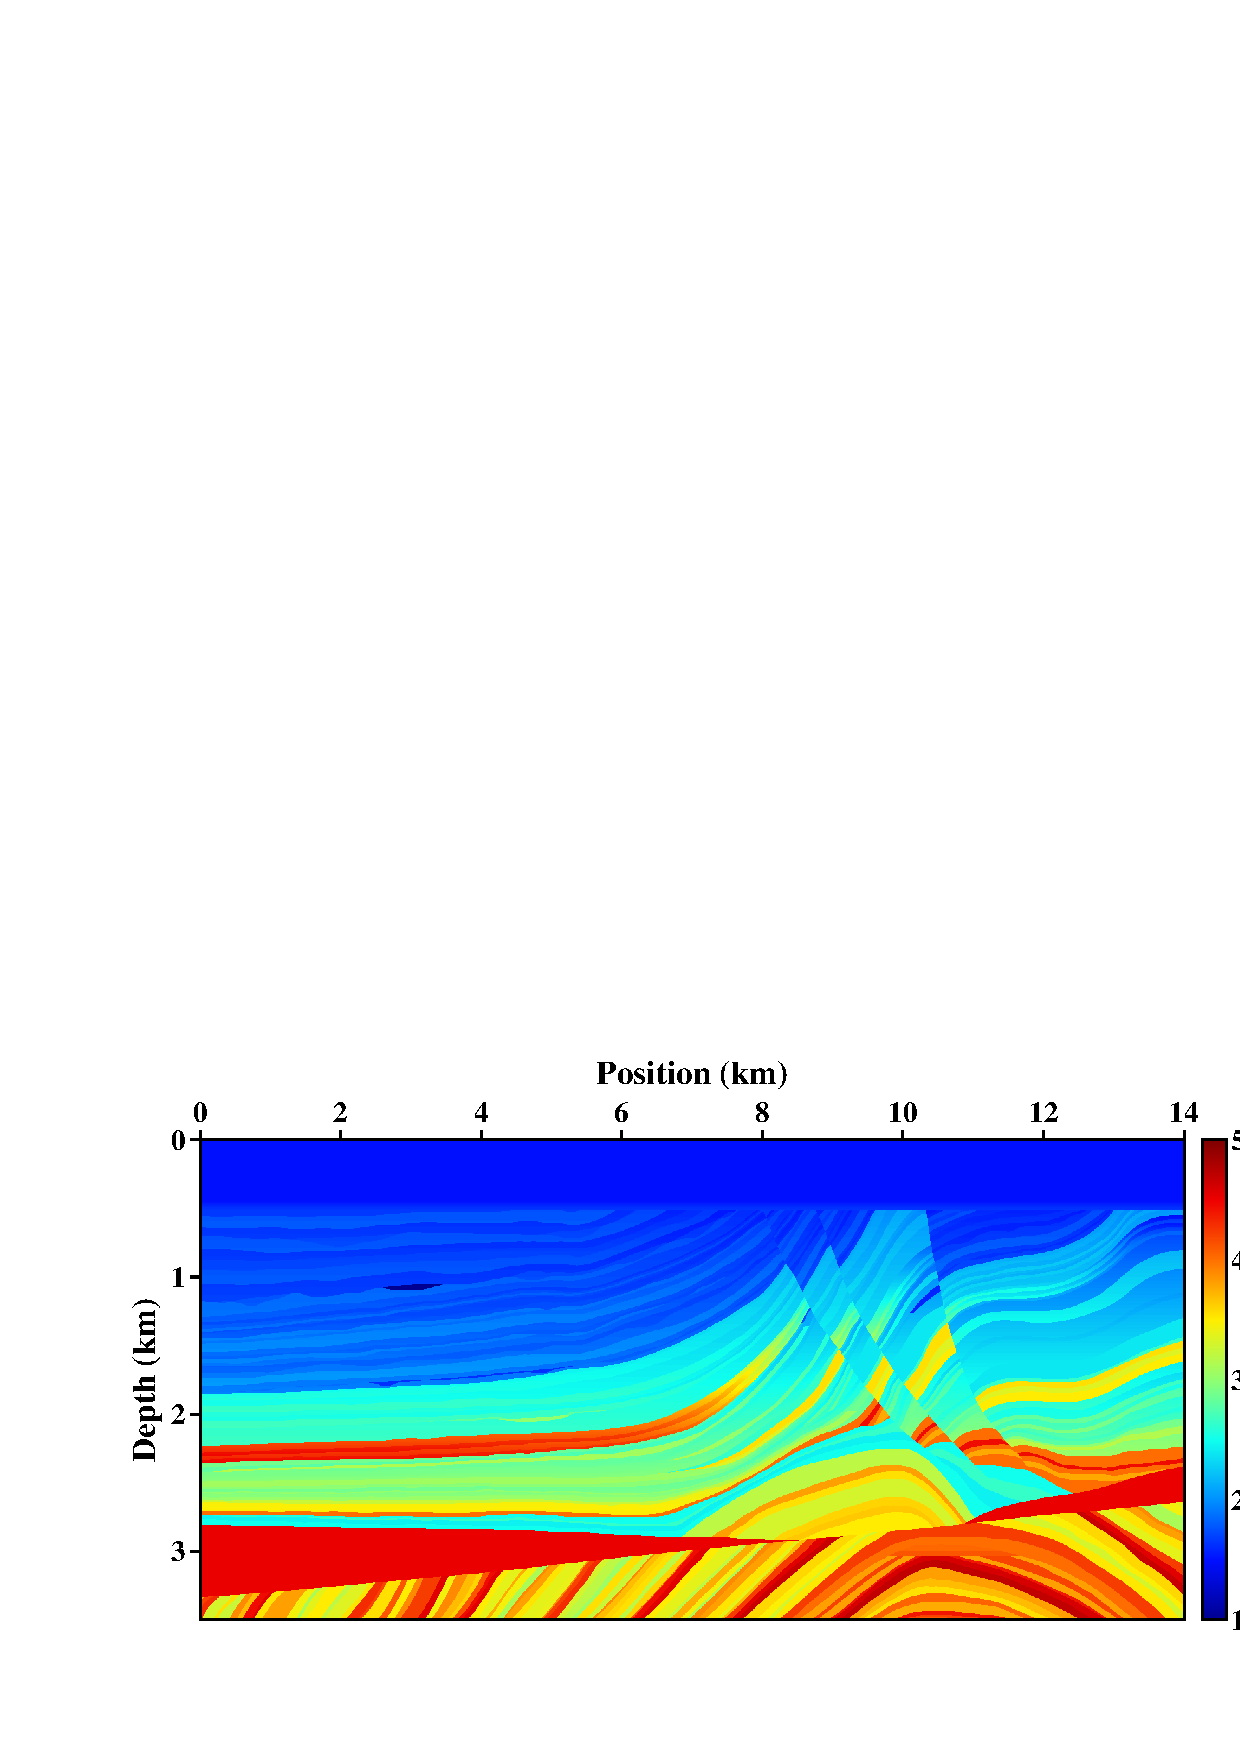
\includegraphics[width=9cm]{tariqsugresult/Fig/truevp.pdf}}
        \subfloat(b){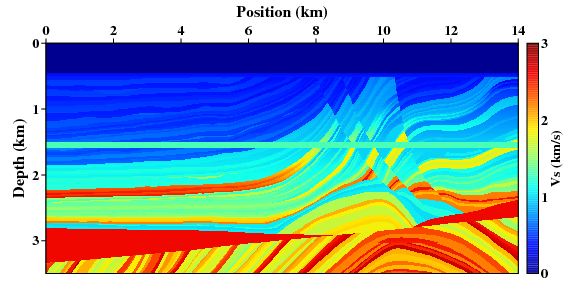
\includegraphics[width=9cm]{tariqsugresult/Fig/truevs.pdf}}
        \subfloat(c){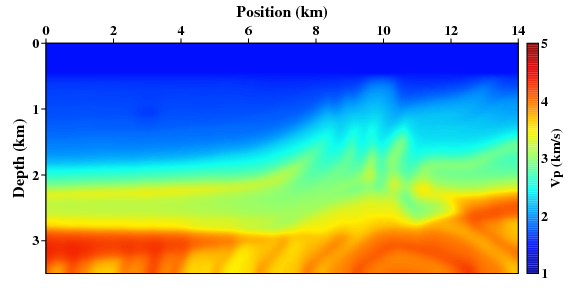
\includegraphics[width=9cm]{tariqsugresult/Fig/initvp.pdf}}
        \subfloat(d){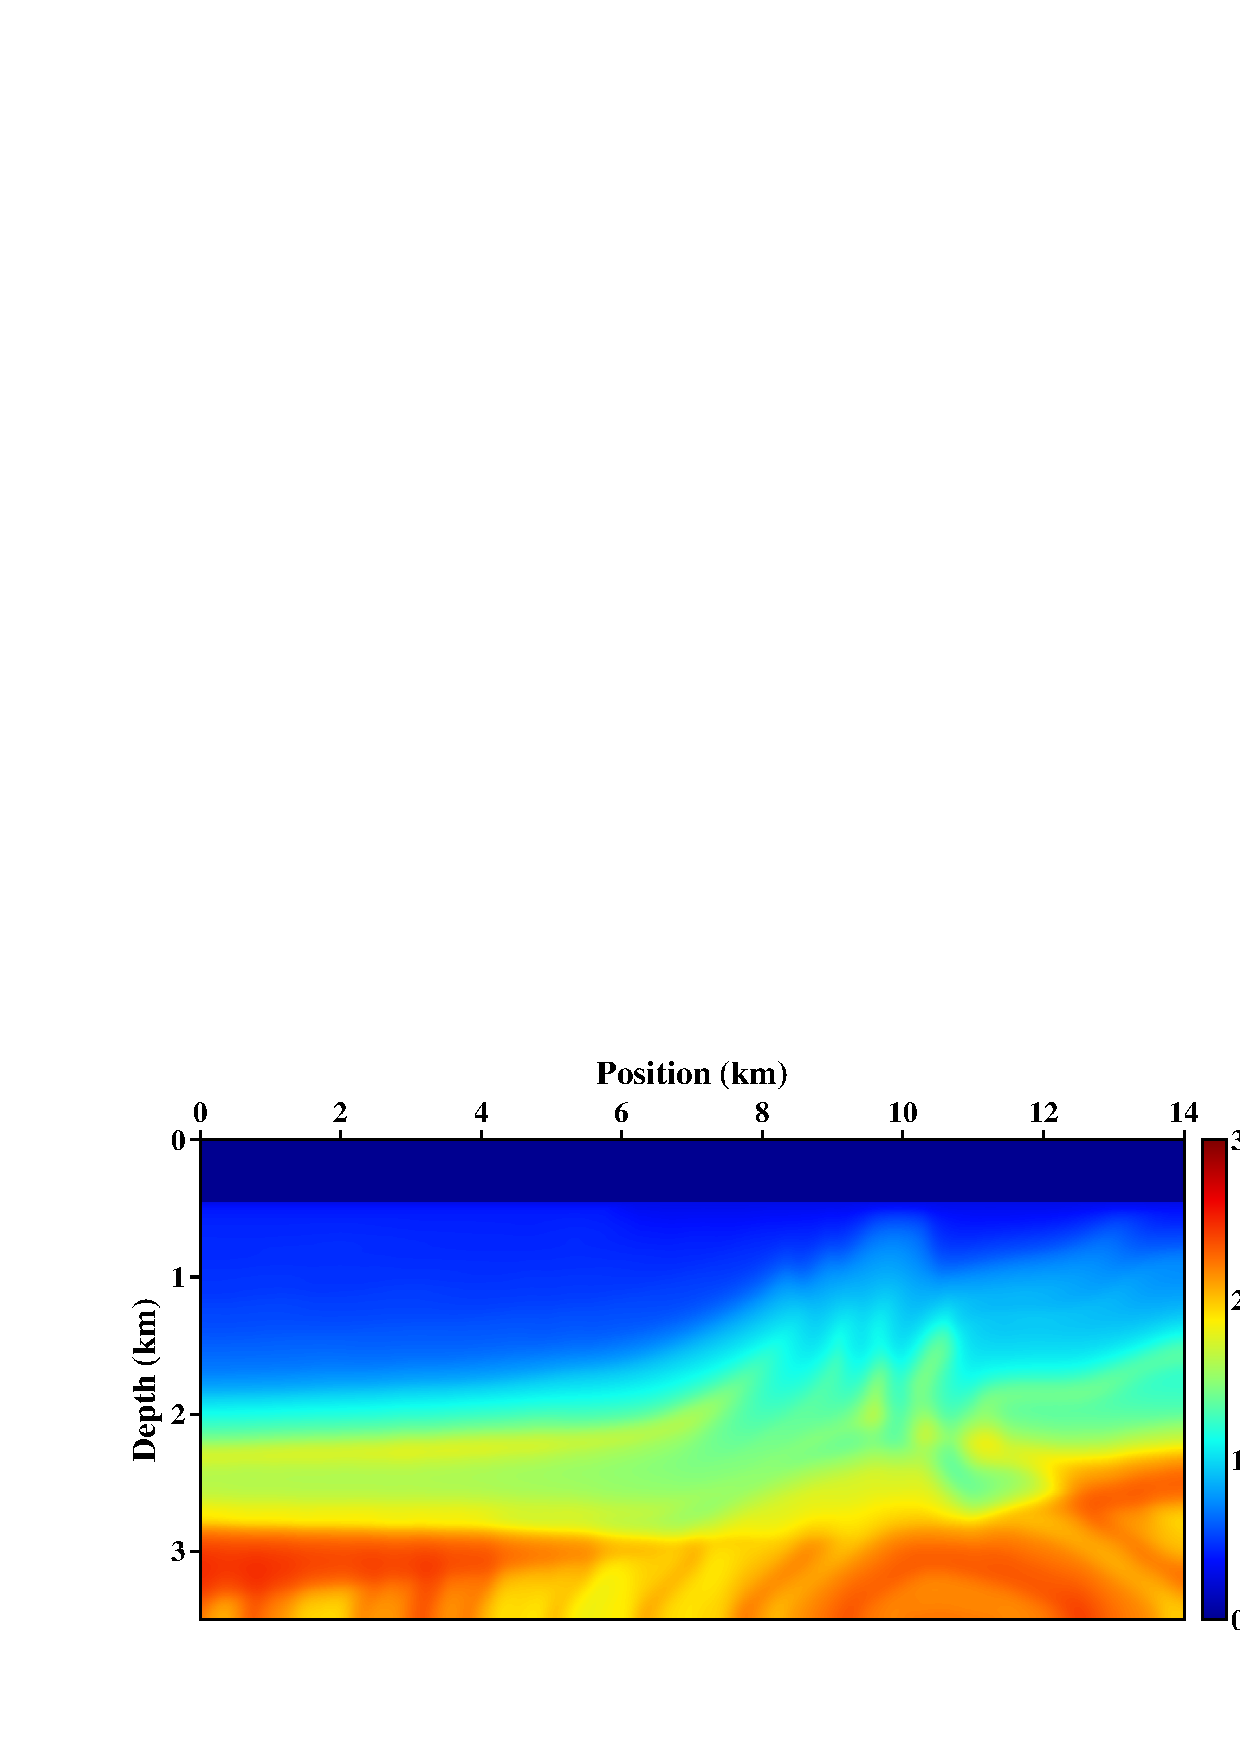
\includegraphics[width=9cm]{tariqsugresult/Fig/initvs.pdf}}
        \caption{
            The SEG Marmousi-II model: (a) and (b) are true $V_p$ and $V_s$ models, respectively,
            while (c) and (d) are initial $V_p$ and $V_s$ models, respectively.
            Note the P-wave velocity
            anomalies related to the gas sand reservoirs and the newly inserted high-velocity
            thin layer in the S-wave velocity field.
    }
    \label{fig:MarInitTrue}
    \end{center}
\end{figure*}
\begin{figure*}
    \begin{center}
        \subfloat(a){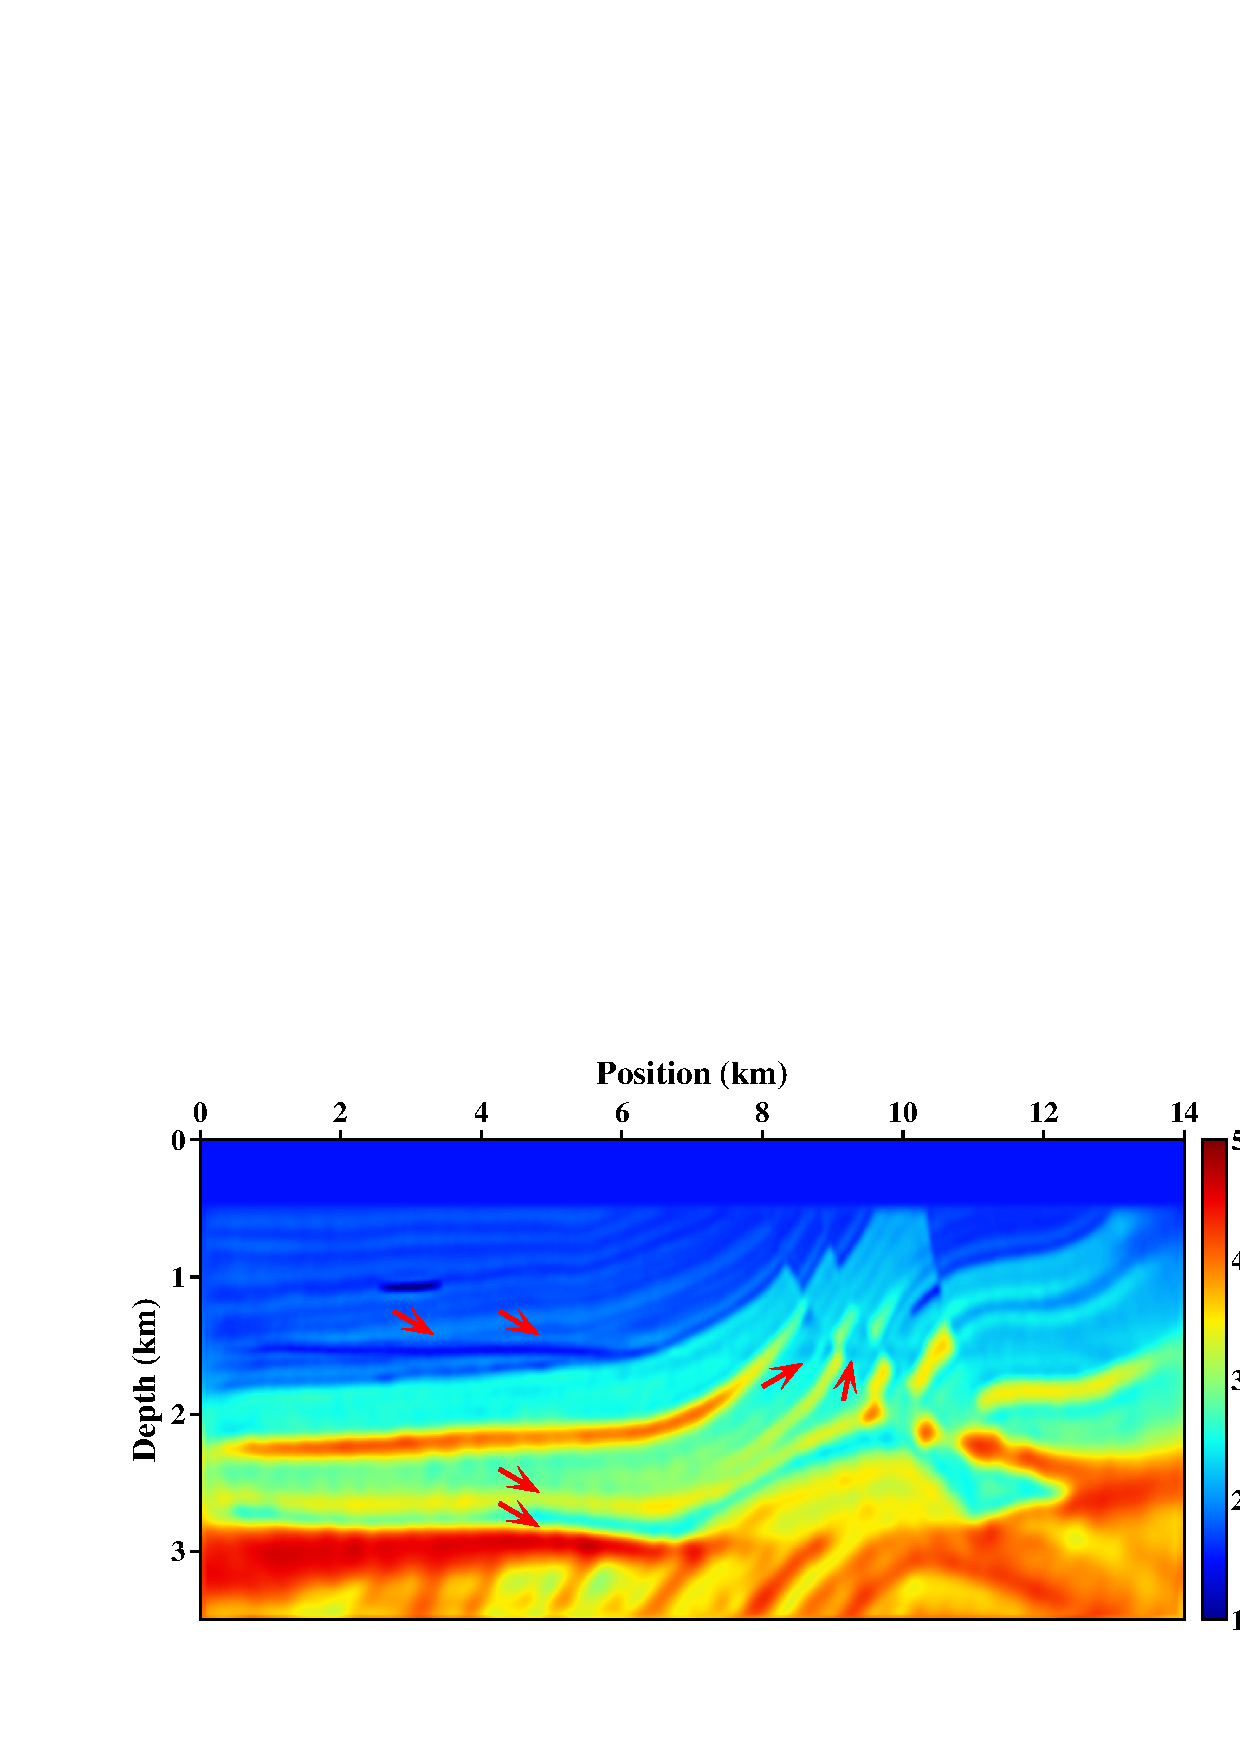
\includegraphics[width=6cm]{tariqsugresult/Fig/nodevp.pdf}}
        \subfloat(b){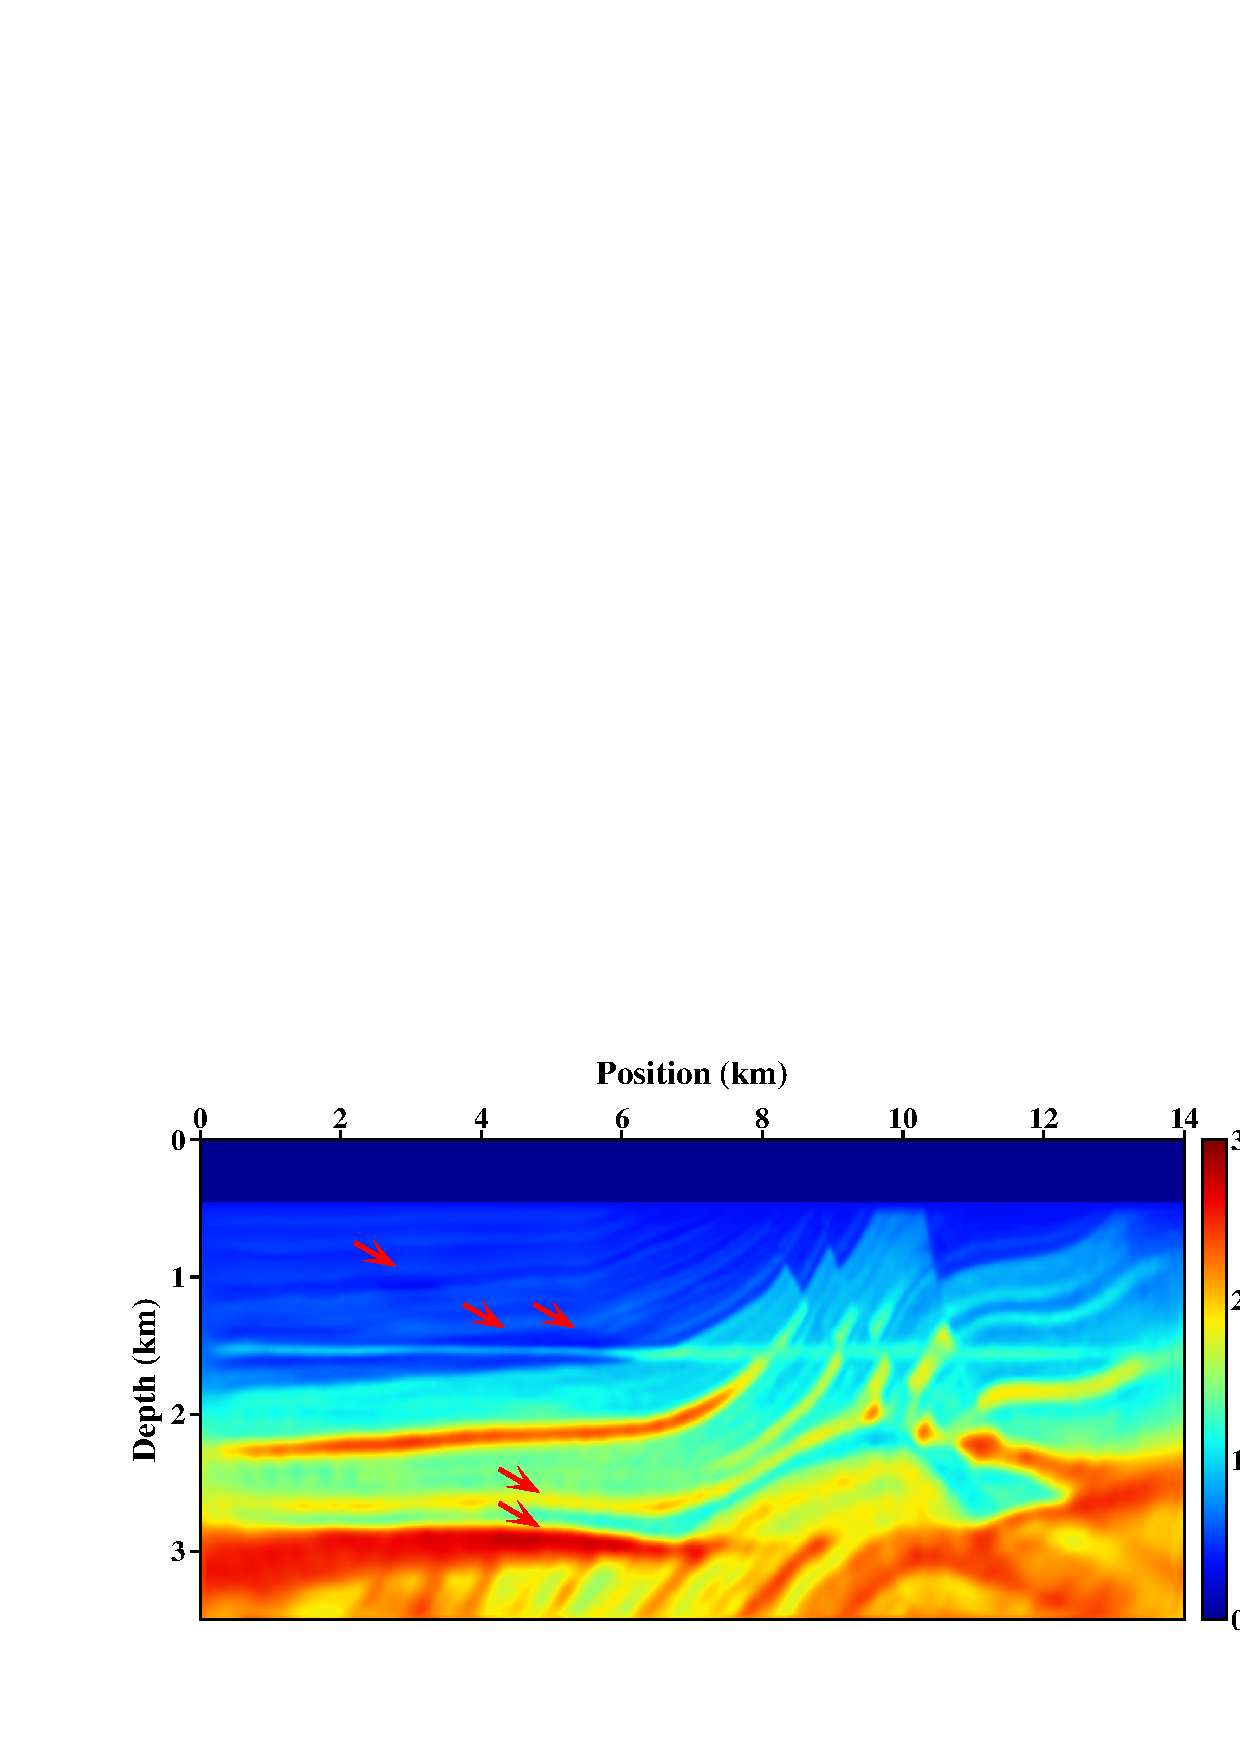
\includegraphics[width=6cm]{tariqsugresult/Fig/nodevs.pdf}}
        \subfloat(c){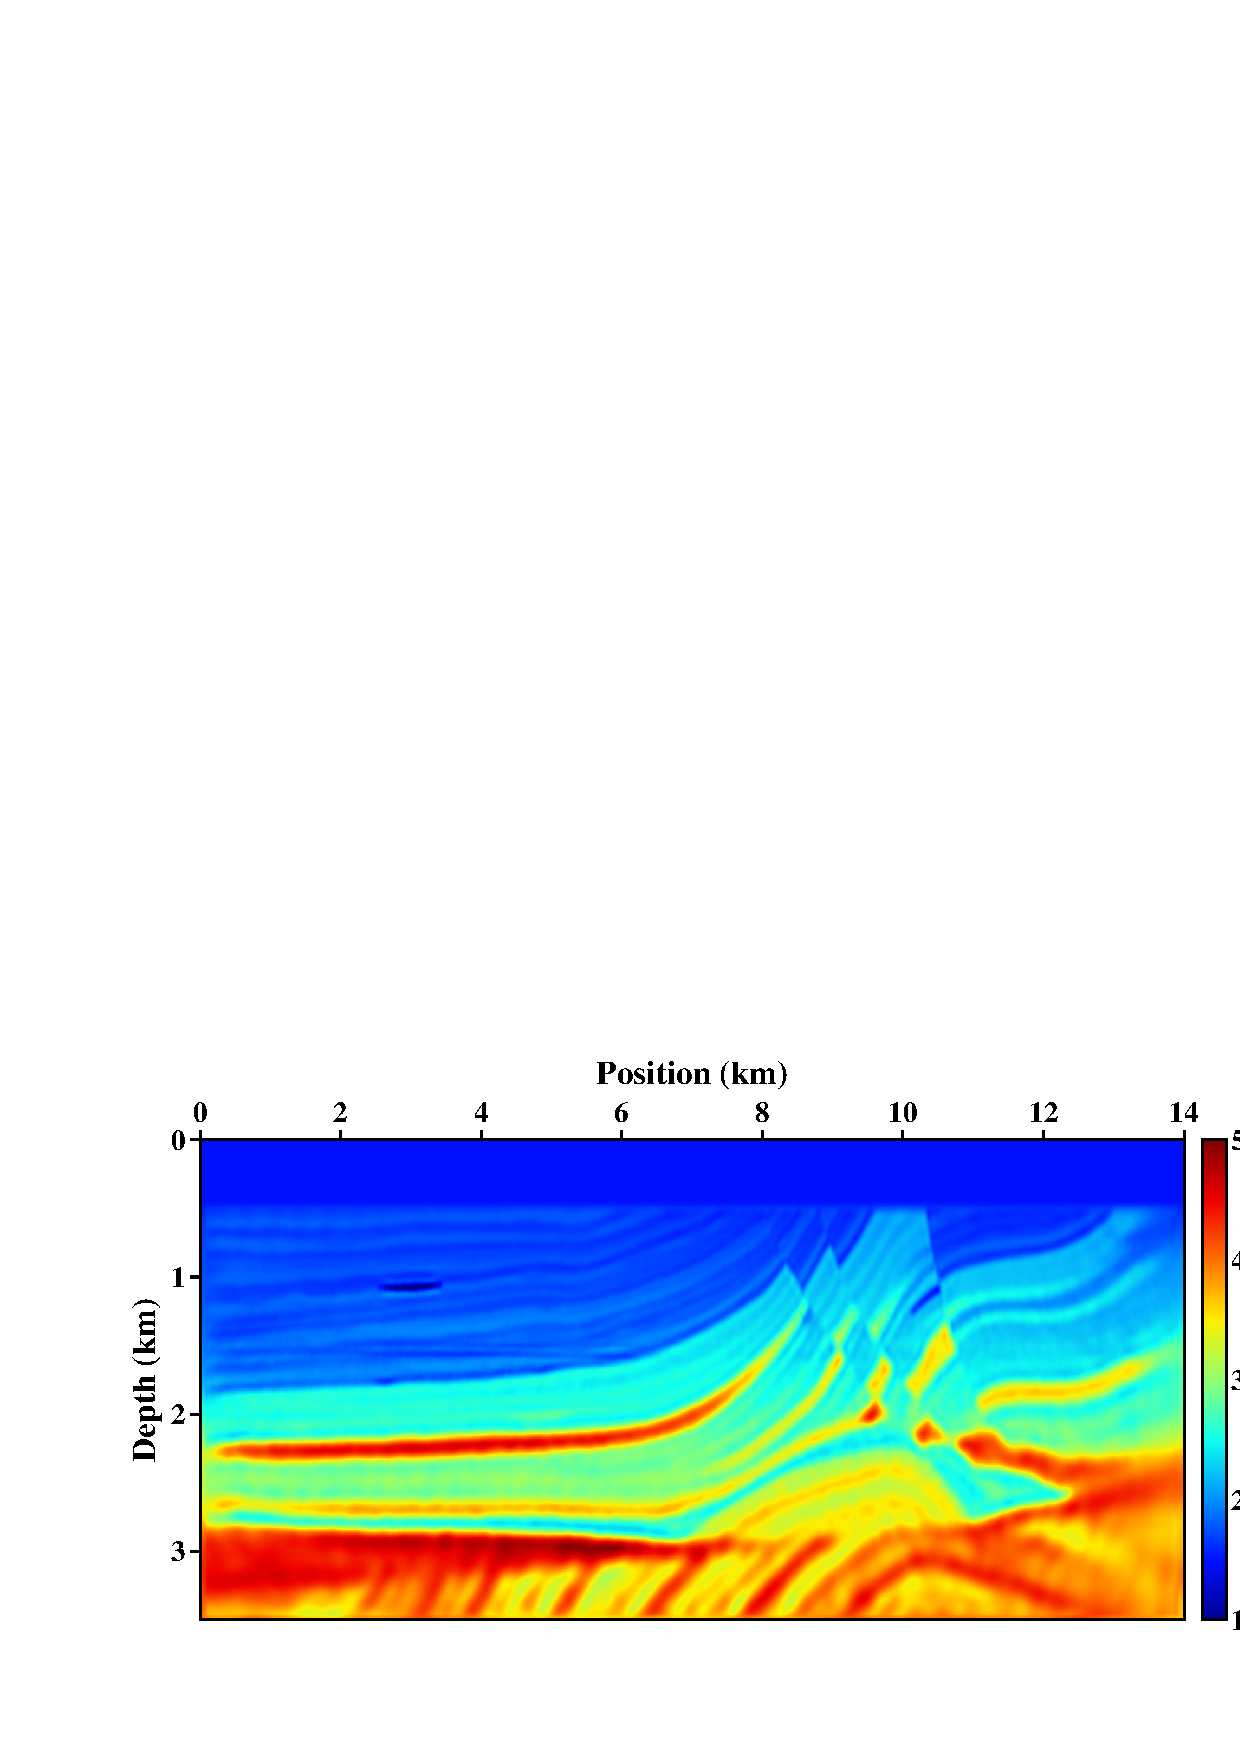
\includegraphics[width=6cm]{tariqsugresult/Fig/devp.pdf}}
        \subfloat(d){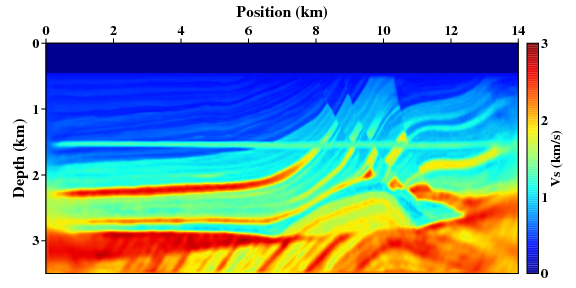
\includegraphics[width=6cm]{tariqsugresult/Fig/devs.pdf}}
        \caption{
        The inverted Marmousi-II model: The inverted results using the PCG (a, b)
            and the MD-based methods (c, d).
        (a) and (c) are $V_p$ models while (b) and (d) are $V_s$ models.
    }
    \label{fig:MarInvert}
    \end{center}
\end{figure*}


图\ref{fig:MarInvert}展示了MD方法比常规方法能提供更好的反演结果。在模型浅部(约1.5km),两种方法都能很好的恢复$V_p$模型,而常规方法恢复的$V_s$模型
分辨率较低一些。很明显,常规方法中,S波速度模型中的高速异常薄层给反演造成了很大的挑战。如图\ref{fig:MarInvert}(a)和(b)中所示,反演结果受到了很强的参数耦合
的干扰,尤其是在左侧的高速异常薄层区域。这就导致了在该异常薄层下方构造的错位与不聚焦,如图中箭头所示。然而,模式解耦反演方法很好地避免了这些参数耦合效应,
获得了模型的细节,包括中部的断层与背斜构造。模型的纵向剖面进一步证明了模式解耦反演方法获得了比常规方法更好的结果。

\begin{figure*}
    \begin{center}
        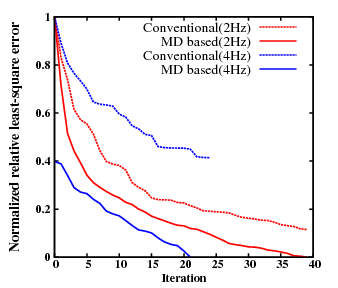
\includegraphics[width=8cm]{tariqsugresult/Fig/L2.pdf}
        \caption{
            Normalized L2 norms as a function of iteration for the PCG-based (dash)
            and MD-based (solid) inversions in the first (red) and second (blue)
            stages.
    }
    \label{fig:L2}
    \end{center}
\end{figure*}
图\ref{fig:L2}展示了在前两个阶段的反演中,归一化的目标函数值随迭代次数的下降曲线。可以看到,模式解耦反演方法要比常规方法收敛更快。在第一个阶段,模式解耦
反演方法的数据拟合程度更高,同时获得了更准确的中低波数模型更新。在第二个阶段,常规梯度方法最终在25次迭代之后停止更新且数据残差相当大,而模式解耦反演方法
在22次迭代后数据残差快速下降达到终止条件。这些结果说明利用模式解耦对梯度做预条件可以很有效地在反演中降低参数耦合从而加速收敛。表\ref{table:TotalComputime}
中列出了在8节点(每节点15核)的工作站上每个阶段的迭代次数和总的计算时间。每个阶段我们设定最大迭代次数为40次。因为当搜索不到合适步长的时候迭代会自动终止,所以
不同阶段的实际迭代次数并不相同。在常规方法中,严重的参数耦合效应会影响从低频数据中重建出合适的宏观模型,这就导致在高频阶段无法获得合理的梯度方向,使得迭代过早终止。而模式解耦方法可以一定程度回避参数耦合,因此其在低频阶段能够重建出合适的宏观模型,从而使得高频阶段的梯度更合理,迭代次数更多。这也是为什么模式解耦方法能
获得更准确,分辨率更高的反演结果。总的来说,模式解耦方法需要更多的迭代次数,也因此计算时间更多。但是每次迭代的平均用时只增加了18\%左右。
\begin{table}
    \caption{The total computational costs}
    \label{table:TotalComputime}
%   \begin{tabular}{|c|c|c|c|c|c|c|}
%   \begin{tabular}{|p{1.8cm}|c|c|c|c|p{2.2cm}p{2.3cm}p{2cm}|}
    \begin{tabular}{p{1.8cm}p{1.0cm}p{1.0cm}p{1.0cm}p{1.2cm}p{1.0cm}p{1.0cm}}
%    \begin{tabular}{|p{1.8cm}|p{1.0cm}p{1.0cm}p{1.0cm}p{1.2cm}|p{1.0cm}p{1.0cm}|}
    \hline
    \quad&\multicolumn{4}{c}{Iteration number}&\multicolumn{2}{c}{Time spent (hour)} \\
%   \quad&\multicolumn{4}{|c|}{Iteration number}&\multicolumn{2}{|c|}{Computing Time (hour)} \\
    \hline
%   Method & stage1 0-2Hz &stage2 0-4Hz&stage3 0-6Hz&stage4 0-10Hz&Total &Average \\
    \multirow{2}{*}{Method} & stage1 &stage2 &stage3 &stage4 &\multirow{2}{*}{Total}
    &\multirow{2}{*}{Average} \\
    & 0-2Hz &0-4Hz&0-6Hz&0-10Hz\\
    \hline
    Conventional&  40   &25&5& 7  &41.4&0.538\\
    MD-based &   40  & 22 &33 &13&68.3&0.632\\
    \hline
    \end{tabular}
\end{table}
\section{讨论}
\subsection{更进一步分解梯度的必要性}
我们可以对正传与反传波场分别解耦从而获得对应不同模式转换的解耦梯度,也即PP、PS、SP和SS。但是,很难设计出一个单独使用某一模式转换数据的EFWI策略,因为我们无法
采用P/S分离的算法在观测面上区分入射波场的类型,也即无法区分PP与SP(或PS与SS)。否则,只能使用分解后的单模式地震数据来进行单参数反演。例如
Ren和Liu\cite{ren.liu:2016},在其四步反演策略的第二步中,当有很强的S波能量时,只采用分解的P波场来反演P波速度,或者在弱S波能量时仅仅拟合S波数据来反演S波速度。
\begin{figure*}
    \begin{center}
        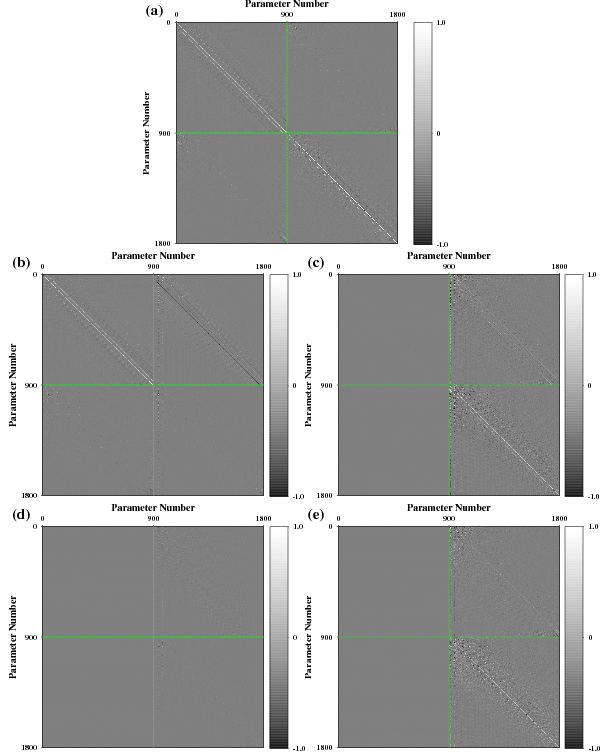
\includegraphics[width=12cm]{ResoOpera/Fig/resolutionMN.pdf}
        \caption{
            Resolution matrices associated with different mode conversion data using
            mix-source:
            (a) $\mathbf{R}$, (b) $\mathbf{R}^{PP}$, (c) $\mathbf{R}^{PS}$, (d)
            $\mathbf{R}^{SP}$ and (e)
            $\mathbf{R}^{SS}$.
    }
    \label{fig:ResoMN}
    \end{center}
\end{figure*}

\begin{figure*}
    \begin{center}
        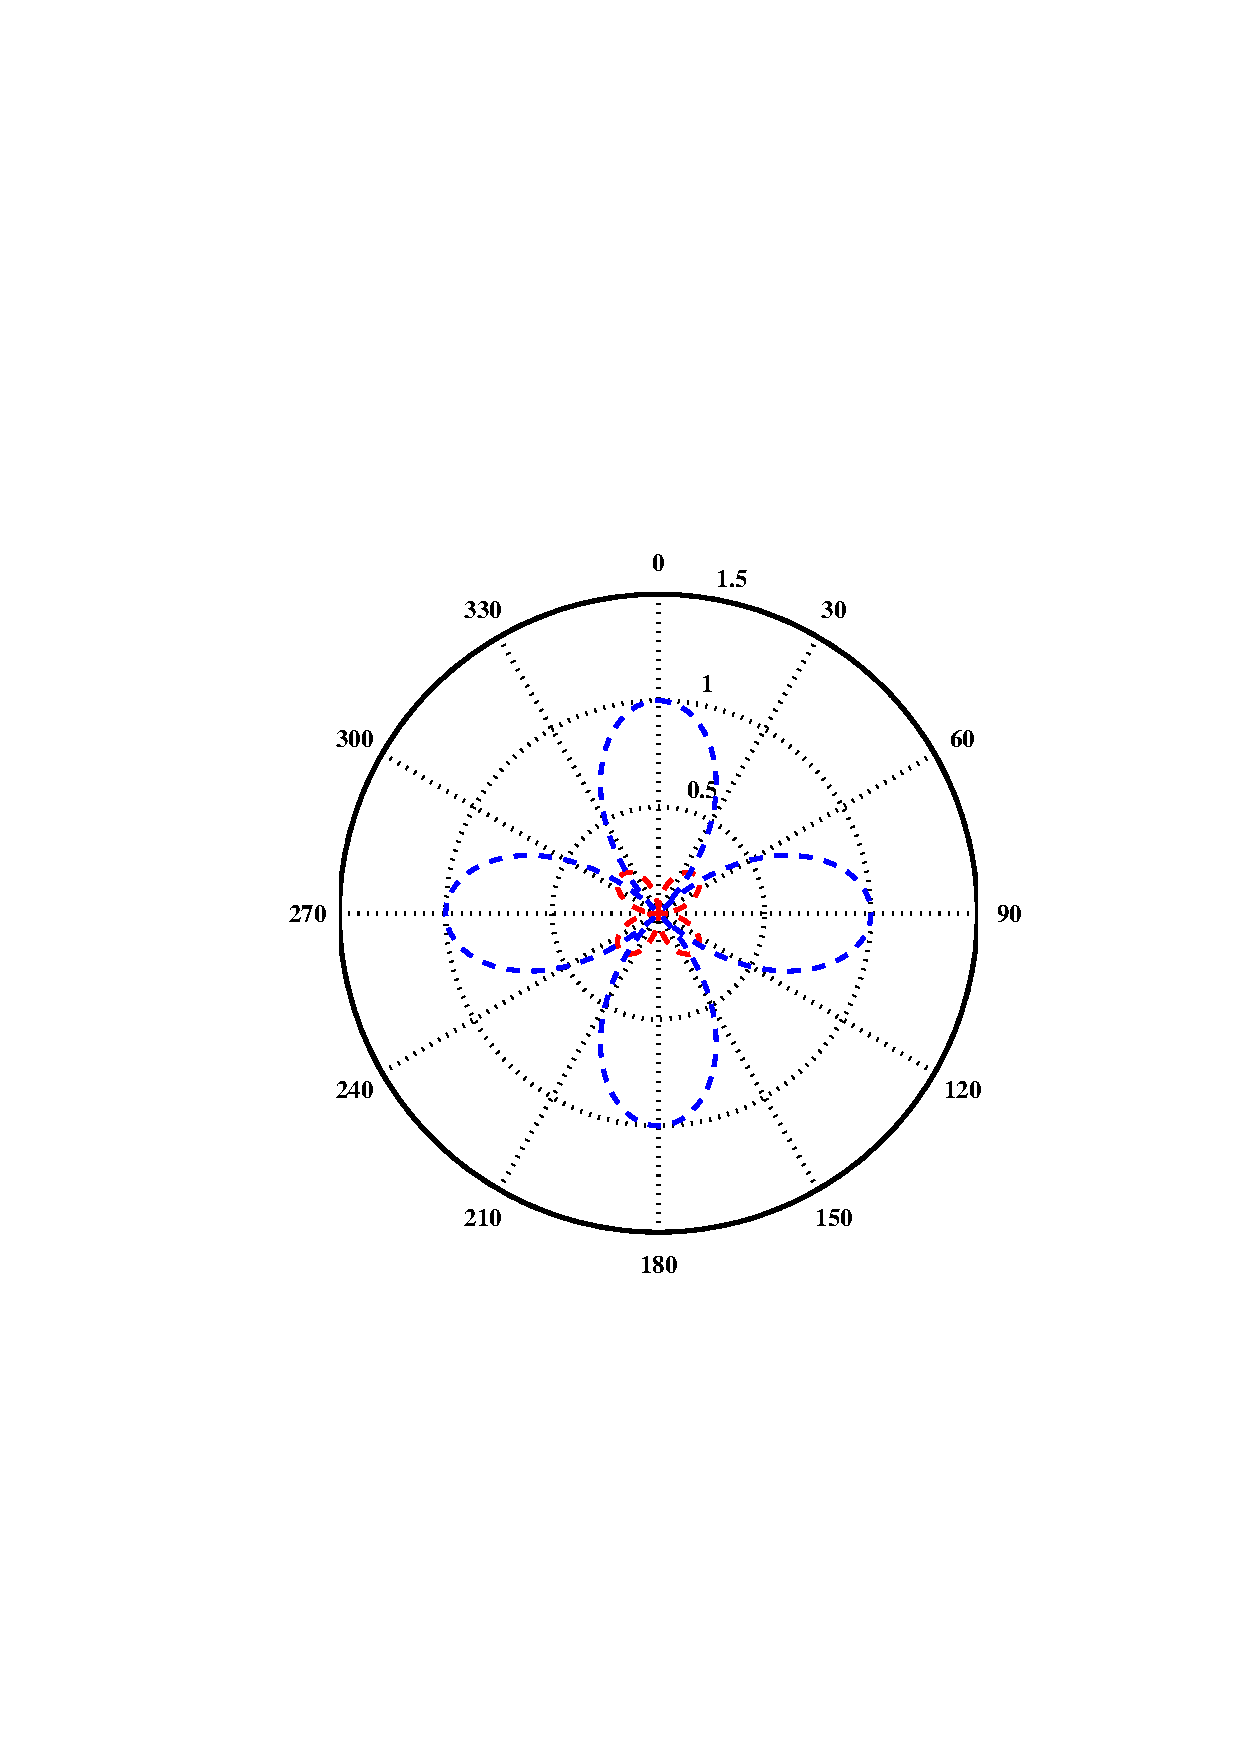
\includegraphics[width=5cm]{radiationpattern/Fig/SPSS.pdf}
        \caption{
            Radiation pattern of SP and SS modes with a same normalization: SP
            mode (red) and SS mode (blue).
    }
    \label{fig:SPSS}
    \end{center}
\end{figure*}


注意到,在梯度计算中分解正传波场等价于次级源(或背景波场)的波模式,而次级源是Frech{$\acute{e}$}t导数中的一部分。因此我们可以将该线性问题写为:
\begin{equation}
    \mathbf{J}^{XY}\delta\mathbf{m}=\mathbf{\delta u}^{XY},
    \label{eq:JXY}
\end{equation}
其中$X$和$Y$分别表示次级源与散射Green's函数的波模式,$\mathbf{\delta u}^{XY}$则表示${X}$-to-${Y}$模式的扰动波场。根据方程\eqref{eq:ResoOperP}的推导方式,我们
可以获得相应的分辨率矩阵:
\begin{equation}
    \mathbf{R}^{XY}=\mathbf{H}_a^{-g}\mathbf{J}^{\dagger}\mathbf{J}^{XY}. 
    \label{eq:RXY}  
\end{equation}
图\ref{fig:ResoMN}展示了PP、PS、SP和SS模式的分辨率矩阵,其观测系统与图\ref{fig:Resolution}中一致,但是采用了P和S的混合震源。图中的带对角结果是由于更加复杂的
波现象。可以看到,$\mathbf{R}^{PP}$ 与$\mathbf{R}^P$十分类似,而$\mathbf{R}^{SP}$却几乎为空矩阵。这表明用PP波数据来反演$V_p$会受到来自$V_s$的干扰。而SP波数据
则对两个参数的反演都贡献很小。从Ren和Liu\cite{ren.liu:2016}的例子中(见其文中图19与20),即使震源中含有足够强的S波能量,SP梯度也是很弱且有很多噪音。一个
可能的解释就是如图\ref{fig:SPSS}所示,S-to-P的散射能量很弱。此外,我们也很那区分出PS和SS模式的贡献,因为从图\ref{fig:ResoMN}中看到,$\mathbf{R}^{PS}$和
$\mathbf{R}^{SS}$的非零元素分布非常一致。因此,想通过分解正传波来对进一步地降低参数耦合效应的潜力非常有限,尽管这样会带来更多的计算量。这也是为什么我们只
分解反传波场来对梯度进行预条件。
\subsection{密度模型的反演}
密度扰动同时散射P-和S-波,但是却几乎不影响两种波模式的相位或者走时。这种模式的散射能量大多与入射波场的传播方向相反\cite[]{wu.aki:1985,tarantola:1986}。因此,
密度作为一个次级效应的参数,由于其微弱的敏感性和多参数的耦合效应\cite[]{tarantola:1986,forgues.lambare:1997},其很难被重构。这也是为何很多EFWI的研究只考虑
常密度的情形\cite[]{shipp:2002,sears:2008,brossier2009}。只有很少一部分的工作能够从多尺度策略和(或)不同参数化方式的选取中获得较为合理的密度反演结果
\cite{jeong2012full}。最近,基于子空间的方式\cite[]{kennett:1988},Xu和McMechan\cite{xu.mcmechan:2014}提出了一种多步长的梯度类方法来压制$V_p$, $V_s$和
$\rho$之间的串扰。Yang等\cite{yang:2016}采用改进的散射积分法(SI)来通过Hessian的逆来提高声波FWI中$V_p$和$\rho$的估计。尽管Ren和Liu\cite{ren.liu:2016}提出了
基于波场解耦的四阶段多尺度策略来做EFWI,但是他们只是在第二阶段中采用了P/S分离来压制$V_p$和$V_s$之间的耦合,然后通过多步长的手段来改善三参数同时反演的结果。




主要大事件:
\begin{itemize}
    \item V1(1971):第一版的UNIX,以~PDP-11/20的汇编语言写成。
        包括文件系统,~fork、roff、ed~等软件。
    \item V4(1973):以~C~语言从头写过,这使得~UNIX~修改容易,可以在几个月内移
        植到新的硬件平台上。最初C语言是为~UNIX~设计的,所以~C~与~UNIX~间有紧密的关系。
    \item V6(1975):第一个在贝尔实验室外(尤其是大学中)广为流传的~UNIX~版本。
        这也是~UNIX~分支的起点与广受欢迎的开始。1.xBSD (PDP-II)就是由这个版本衍生出来的。
    \item V7(1979):在许多UNIX玩家的心目中,这是“最后一个真正的~UNIX,”
        这个版本包括一个完整的~K\&RC~编译器,Bourne
        shell。V7~移植到~VAX~机器后称为~32V。
\end{itemize}


%%% Local Variables:
%%% mode: latex
%%% TeX-master: t
%%% End:



\chapter{弹性波波动方程反射FWI走时反演}

\section{引言}
在第1章中,我们知道
EFWI可以提供高精度地下模型参数估计,但是需要有非常好的初始模型。走时反演只利用了走时残差,而走时残差与低波数成分的模型扰动具有更强的线性关系,所以这两者的联系
会更敏感。因此,采用弹性波波动放程反射走时反演(WERTI)来建立P和S波速度的初始模型将会更加稳健且有效,尤其是对深部的宏观结构恢复更有帮助。在弹性介质中,为了区
分P和S波的反射走时,我们将地面地震数据分解为矢量的P-和S-波地震记录。反射P波与S波的走时信息采用Dynamic
image
warping(DIW)的方式来获取。我们首先采用P波走时来反演P波速度,其次采用S波走时来反演S波速度。
在此过程中,我们采用模式解耦来求取预条件的梯度。Sigsbee2A模型的数值实验例子证明了我们的方法可以有效得获取模型长波长信息。

\subsection{引言}
弹性波全波形反演可以提供高精度的地下模型参数估计,但是也同样受困于多参数反演中的强烈非线性程度以及声波情况下的周波跳跃问题\cite[]{sears:2008,brossier2009}。
Xu et al. (2012)\cite{xu:2012}提出一种反射波波形反演(RWI)的方法,其通过采用偏移/反偏移的方式来预测反射波,从而估计模型中的长波长成分。采用拟合波形的思路,近期
Wu and Alkhalifah (2015)\cite[]{Wu2015b}以及Zhou et al. (2015)\cite[]{Zhou2015}发展了该RWI方法,而Guo and Alkhalifah (2016)\cite{Guo2016}则将该方法扩展到了
弹性介质中。

尽管波形信息能提高反演精度,但是走时信息对模型的低波数成分扰动更敏感,二者之间具有更好的线性关系。所以,采用走时反演来为常规FWI建立合适的含有长波长信息的初始
模型会更加稳健有效\cite[]{Ma2013, Chi2015, Luo2016}。然而在弹性介质中,这中思路会受到限制,因为弹性波场中存在复杂的模式转换,这就导致很难获得单一波模式的走时
信息。在本文中,我们将致力于通过波模式解耦和“动态图像打开”(DIW)\cite[]{Ma2013}来区分出PP和PS的反射走时。之后,我们利用区分出的PP和PS反射走时,通过一个两步
的反演流程来实现WERTI\cite[]{Hale2013}。最后,最后,Sigsbee2A模型的数值实验结果证明了弹性波WERTI方法的有效性。
\subsection{弹性WERTI方法的目标函数和梯度}
假设在背景弹性介质$c_{ijkl}$中有一个参数扰动$\delta c_{ijkl}$,则背景波场与扰动波场满足以下方程:
\begin{equation}
    \rho \frac{\partial u^2_i}{\partial t^2}  -
    \frac{\partial}{\partial x_j}\left[ 
        c_{ijkl}\frac{\partial u_{k}}{\partial
        x_l}\right]=f_i,
    \label{eq:WE} 
\end{equation}
和
\begin{equation}
    \rho \frac{\partial \delta u^2_i}{\partial t^2}  -
    \frac{\partial}{\partial x_j}\left[ 
        c_{ijkl}\frac{\partial \delta u_{k}}{\partial
        x_l}\right]=\frac{\partial}{\partial x_j}\left[\delta c_{ijkl}\frac{\partial u_{k}}{\partial x_l}\right],
    \label{eq:DeltaWE} 
\end{equation}
其中,$\delta u_i$可以看作是用RTM或其他方法的成像结果,$\delta c_{ijkl}$进行反偏移之后的反射数据。在WERTI中,我们需要使得观测数据$\mathbf{d}^{o}$与模拟数据
$\mathbf{d}^{c}$之间的走时残差最小,则目标函数为:
\begin{equation}
    E=\frac{1}{2}\int\tau^2(\mathbf{x_r},t;\mathbf{x_s})dtd\mathbf{x_r}d\mathbf{x_s},
    \label{eq:Objectivefunction} 
\end{equation}
其中,走时残差$\tau(\mathbf{x_r},t;\mathbf{x_s})$可以通过DIW来获取。通过类似Ma and
Hale (2013)\cite{Ma2013}的推导(见附录\ref{cha:AdjointForEWERTI}),我们可以得到如下梯度公式:
\begin{equation}
    \frac{\partial E}{\partial c_{ijkl}}=-\int (\frac{\partial u_{i}}{\partial
    x_j}\frac{\partial \delta \psi_{k}}{\partial x_l}+\frac{\partial \delta u_{i}}{\partial
    x_j}\frac{\partial \psi_{k}}{\partial x_l}),
    \label{eq:GradientCijkl}
\end{equation}
其中,$\psi_i$和$\delta \psi_i$是共轭波场满足:
\begin{equation}
    \rho \frac{\partial \psi^2_i}{\partial t^2}  -
    \frac{\partial}{\partial x_j}\left[ 
        c_{ijkl}\frac{\partial \psi_{k}}{\partial
        x_l}\right]=\tau(\mathbf{x_r},t;\mathbf{x_s})\frac{\dot{d}^o_i(\mathbf{x_r},t+\tau;\mathbf{x_s})}{h_i(\mathbf{x_r},t;\mathbf{x_s})},
    \label{eq:AdjointWE} 
\end{equation}
和
\begin{equation}
    \rho \frac{\partial \delta \psi^2_i}{\partial t^2}  -
    \frac{\partial}{\partial x_j}\left[ 
        c_{ijkl}\frac{\partial \delta \psi_{k}}{\partial 
        x_l}\right]=\frac{\partial}{\partial x_j}\left[\delta c_{ijkl}\frac{\partial
        \psi_{k}}{\partial x_l}\right], 
    \label{eq:AdjointDeltaWE} 
\end{equation}
上式中$h_i(\mathbf{x_r},t;\mathbf{x_s})=(\dot{d}^o_i(\mathbf{x_r},t+\tau;\mathbf{x_s}))^2-\ddot{d}^o_i(\mathbf{x_r},t+\tau;\mathbf{x_s})
(d^c_i(\mathbf{x_r},t;\mathbf{x_s})-d^o_i(\mathbf{x_r},t+\tau;\mathbf{x_s}))$,而$\dot{d}$则代表$d$在时间方向的导数。在方程\eqref{eq:GradientCijkl}的右端项
中,第一和第二项分别表示震源端和检波点端的反射波路径。之后我们可以通过链式法则来导出P波与S波速度的梯度公式:
\begin{equation}
    \frac{\partial E}{\partial V_p}=2\rho V_p\frac{\partial E}{\partial
        c_{ijkl}}\delta_{ij}\delta_{kl}, \qquad
    \frac{\partial E}{\partial V_s}=2\rho V_s\frac{\partial
    E}{\partial c_{ijkl}}(-2\delta_{ij}\delta_{kl}+\delta_{ik}\delta_{jl}+
    \delta_{il}\delta_{jk}).
    \label{eq:GradientVel}
\end{equation}
\subsection{弹性波WERTI工作流程}
弹性波介质中,不同模式的转换波,主要是PP与PS同相轴之间,会互相叠加、互相交叉。在用DIW提取走时差的时候,这些交叉点的位置就会变成一些奇异点而给拾取带来很大困难
。因此,如果直接用原始多分量数据的话,拾取到的$\tau(\mathbf{x_r},t;\mathbf{x_s})$就会不准确,这也是为什么式\eqref{eq:AdjointDeltaWE}中的梯度很难直接应用。
为了解决这个问题,我们将观测与模拟地震数据分解为P波与S波两部分。该模式分解只作用于地面地震数据\cite[]{Li2016a},因此我们可以快速地获得每一炮数据分解之后的矢量
P波或S波地震记录。这样,走时残差就可以被分成P波与S波两部分,使得弹性波WERTI变得可行,也即用一个两阶段的流程,先P波阶段后S波阶段。

在P波阶段,主要采用PP反射波来建立P波速度的背景模型。首先,我们从ERTM中获得P波速度的扰动,也即$\delta V_p$。由于在WERTI中我们只考虑走时,所以我们只进行ERTM成像
而不是最小平方ERTM来拟合反射波振幅。因此,目标函数可以变做最小化PP反射波的走时残差:
\begin{equation}
    E_{pp}=\frac{1}{2}\int\tau^2_{pp}(\mathbf{x_r},t;\mathbf{x_s})dtd\mathbf{x_r}d\mathbf{x_s}.
    \label{eq:ObjectivefunctionPP} 
\end{equation}
这样,采用P波记录来计算方程\eqref{eq:AdjointWE}的右端项,并用$\delta V_p$替换方程\eqref{eq:DeltaWE}和\eqref{eq:AdjointDeltaWE}中的$\delta c_{ijkl}$,我们
就可以计算得到$V_p$的梯度, $\frac{\partial E}{\partial V_p}$。

在S波阶段,我们将采用类似的策略但是只利用PS反射波。则目标函数变为:
\begin{equation}
    E_{ps}=\frac{1}{2}\int\tau^2_{ps}(\mathbf{x_r},t;\mathbf{x_s})dtd\mathbf{x_r}d\mathbf{x_s}.
    \label{eq:ObjectivefunctionPS} 
\end{equation}
但是,实现方式与前一阶段策略略有不同。经过P波阶段反演之后,$V_p$的背景速度已经获得了很好的恢复,此时PP波成像结果应该已经比较接近准确位置。而通常情况下,地
下介质中$V_p$与$V_s$的界面是比较一致的。所以,我们推荐采用较为准确的PP成像($\delta V_p$)结果而不是$\delta V_s$来产生PS反射波。此外,在PS反射中,波路径的
震源端只与P波速度相关,因此我们在计算$\frac{\partial E}{\partial V_s}$可以丢掉方程\eqref{eq:GradientCijkl} 右端项的第一部分。并且,波模式分解也会施加在
梯度的计算过程中来确保只有S波能量参与其中:
\begin{equation}
    \frac{\partial E_{ps}}{\partial V_s}=-2\rho V_s
    \int (\frac{\partial \delta u^S_{i}}{\partial
    x_j}\frac{\partial \psi^S_{k}}{\partial x_l})
    (\delta_{ik}\delta_{jl}+
    \delta_{il}\delta_{jk}).
    \label{eq:GradientVel}
\end{equation}
上述梯度与Wang et al. (2015)\cite{Wang2015a}提出的EFWI方法类似。模式解耦可以在$V_s$的反演中降低参数耦合同时也可以压制假象。

\subsection{局部倾角滤波约束}
WERTI非常类似成像域射线走时层析。而我们知道射线走时层析反问题通常不收敛,很难收敛或者很难收敛获得具有地质意义的模型。
在偏移后,成像结果可以提供地下界面大致的倾角信息,通过此类倾角信息,可以设计预条件算子来沿地层倾角来对反演进行约束,使得反演结果更合理。
采用倾角约束滤波可以加快收敛速度,在很大程度上改善反演结果。由于采用波动方程作为手段,WERTI采用波路径信息来反投影走时残差信息,因而其所面临的挑战要
小于射线走时层析。然而,对于一些照明不足,或者
反射路径覆盖不均匀的区域同样也会出现上述的问题。常规的各向同性的平滑算子很难保证反演收敛到具有地质含义的物理模型。因此,WERTI中采用局部倾角约束同样可以加速
收敛,并获得具有地质意义的反演结果。

Hale(2009)采用结构张量来估计地层倾角。对于2D的图像,结构张量是$2\times2$的矩阵:
\begin{equation}
        \mathbf{S}=
        \begin{pmatrix}
                < s^2_1 > \quad <s_1s_2 >\\
                < s_1s_2 > \quad < s^2_2 >\\
        \end{pmatrix},
        \label{eq:StructureTensor}
\end{equation}
其中$s_1$和$s_2$表示图像垂直和水平方向的方向导数,$<\dot>$表示2D的Gaussian平滑函数。上式对应的特征值问题可以表示为:
\begin{equation}
	\mathbf{S}=\lambda_u\mathbf{u}\mathbf{u}^T+\lambda_v\mathbf{v}\mathbf{v}^T
        \label{eq:EigenValueVector}
\end{equation}
其中,$\lambda_u$和$\lambda_v$分别为特征向量$\mathbf{u}$和$\mathbf{v}$对应的特征值。我们定义$\lambda_u\ge\lambda_v\ge0$,这样的话$\mathbf{u}$指示梯度最大的
方向,也即与线性结构垂直的方向。而话$\mathbf{u}$则指示与线性结构平行的方向。Hale(2009)指出,可以设置$\lambda_u(\mathbf{x})=0$
和$\lambda_v(\mathbf{x})=1$,这样保证图像中每一处平滑都会沿倾角方向。则沿倾角平滑的滤波器可以通过以下方程求解:
\begin{equation}
	(\mathbf{B}^T\mathbf{B}+\mathbf{A}^T\mathbf{S}^{\prime}\mathbf{A})\mathbf{h}=\mathbf{B}^T\mathbf{B}\mathbf{f}
        \label{eq:SparseMatrixSystem}
\end{equation}
其中,$\mathbf{S}^{\prime}$为新构造的结构张量,$\mathbf{B}$和$\mathbf{A}$分别为求和算子以及差分算子对应的矩阵,$\mathbf{f}$为输入图像,$\mathbf{h}$
为输出的平滑后图像。该方程可以通过共轭梯度法快速求解。



%%% Local Variables:
%%% mode: latex
%%% TeX-master: t
%%% End:
\chapter{基于模式解耦的弹性波最小平方逆时偏移}
\label{cha:MD-ELSRTM}
\section{引言}
前一章内容中我们将模型分解为高波数与低波数成分,并通过弹性波WERTI方式来恢复模型的低波数成分。常规的FWI算法可以恢复模型的高波数成分,但是会受到许多因素干扰,
如cycle-skipping问题,信噪比低,地震子波未知,正演算子不准确等等。除此之外,我们通常也会通过最小平方偏移(LSM)来实现高波数成分的重构。
早在1993年,Schuster(1993)\cite{Schuster1993}提出了针对井间数据的LSM算法,而Nemeth et al.\cite{Nemeth1999}将该方法应用到了地面数据中。
以波动方程为引擎的最小平方逆时偏移(LSRTM)近年来一直是研究的热点,例如Dai and
Schuster(2013)\cite{Dai2013},Dong et al.(2012)\cite{Dong2012}, Luo and
Hale(2014)\cite{Luo2014}。尽管其计算代价昂贵,但是LSRTM可以回避模型速度复杂时所产生的多路径问题。
LSRTM的过程通常被认为是线性的全波形反演,其假设在已经获得足够好的低波数模型成分之后恢复模型的高频扰动,也即获得“像”,使得在最小平方意义下,
用该“像”所预测的反射数据能与观测数据达到最佳匹配。因此,最小平方逆时偏移与全波形反演的理论框架是一致的。

近期,为了更准确地描述波传播过程,同时获得更多的参数
成像,并解决多参数带来的耦合效应,原本基于声波方程的
LSRTM被推广到了变密度声波介质\cite{Yang2017},衰减介质\cite{Dai2015}以及弹性介质中\cite{Duan2016,Feng2016,Xu2016}(ELSRTM)。
相比声波成像,弹性波成像可以提供更多的地下信息,例如裂缝分布以及弹性性质。但是,弹性波偏移中存在的许多问题会很大程度上影响成像质量。因为通常很难将记录中的
波模式完全区分开,因此其中某些波模式的会因速度不对而被错误地成像。这些非物理的模式就会引起假象,也即“cross-talk”。
而通过ELSRTM则可以提高成像的分辨率,并且可以压制由于观测孔径限制,粗网格采样以及数据缺失引起的偏移假象。
弹性波成像需要处理矢量波的问题,也就需要选取合适的成像条件,{\color{red}\cite{Wang2016}提出了无极性反转的矢量成像条件等等。}而从EFWI理论框架出发,许多学者,
如Duan et al.(2016)\cite{Duan2016},Feng et
al.(2016)\cite{Feng2016}等都推导出了与EFWI梯度非常类似的成像条件。该成像条件也可以回避极性反转问题,同时也可以认为是更加接近于高频的参数扰动梯度。而基于
第二章中对EFWI算法的分析,模式解耦带来的优势将同样能在ELSRTM中得以应用,因此我们将在本章中应用波模式解耦来对ELSRTM进行预条件,从而获得更好结果。
\section{弹性}
假设在背景弹性介质$c_{ijkl}$中有一个参数扰动$\delta c_{ijkl}$,则背景波场与扰动波场满足以下方程:
\begin{equation}
    \rho \frac{\partial u^2_i}{\partial t^2}  -
    \frac{\partial}{\partial x_j}\left[ 
        c_{ijkl}\frac{\partial u_{k}}{\partial
        x_l}\right]=f_i,
    \label{eq:WE} 
\end{equation}
和
\begin{equation}
    \rho \frac{\partial \delta u^2_i}{\partial t^2}  -
    \frac{\partial}{\partial x_j}\left[ 
        c_{ijkl}\frac{\partial \delta u_{k}}{\partial
        x_l}\right]=\frac{\partial}{\partial x_j}\left[\delta c_{ijkl}\frac{\partial u_{k}}{\partial x_l}\right],
    \label{eq:DeltaWE} 
\end{equation}
其中,$\delta u_i$可以看作是用RTM或其他方法的成像结果,$\delta c_{ijkl}$进行反偏移之后的反射数据。在WERTI中,我们需要使得观测数据$\mathbf{d}^{o}$与模拟数据
$\mathbf{d}^{c}$之间的走时残差最小,则目标函数为:
\begin{equation}
    E=\frac{1}{2}\int\tau^2(\mathbf{x_r},t;\mathbf{x_s})dtd\mathbf{x_r}d\mathbf{x_s},
    \label{eq:Objectivefunction} 
\end{equation}
其中,走时残差$\tau(\mathbf{x_r},t;\mathbf{x_s})$可以通过DIW来获取。通过类似Ma and
Hale (2013)\cite{ma2013}的推导(见附录\ref{cha:AdjointForEWERTI}),我们可以得到如下梯度公式:
\begin{equation}
    \frac{\partial E}{\partial c_{ijkl}}=-\int (\frac{\partial u_{i}}{\partial
    x_j}\frac{\partial \delta \psi_{k}}{\partial x_l}+\frac{\partial \delta u_{i}}{\partial
    x_j}\frac{\partial \psi_{k}}{\partial x_l}),
    \label{eq:GradientCijkl}
\end{equation}
其中,$\psi_i$和$\delta \psi_i$是共轭波场满足:
\begin{equation}
    \rho \frac{\partial \psi^2_i}{\partial t^2}  -
    \frac{\partial}{\partial x_j}\left[ 
        c_{ijkl}\frac{\partial \psi_{k}}{\partial
        x_l}\right]=\tau(\mathbf{x_r},t;\mathbf{x_s})\frac{\dot{d}^o_i(\mathbf{x_r},t+\tau;\mathbf{x_s})}{h_i(\mathbf{x_r},t;\mathbf{x_s})},
    \label{eq:AdjointWE} 
\end{equation}
和
\begin{equation}
    \rho \frac{\partial \delta \psi^2_i}{\partial t^2}  -
    \frac{\partial}{\partial x_j}\left[ 
        c_{ijkl}\frac{\partial \delta \psi_{k}}{\partial 
        x_l}\right]=\frac{\partial}{\partial x_j}\left[\delta c_{ijkl}\frac{\partial
        \psi_{k}}{\partial x_l}\right], 
    \label{eq:AdjointDeltaWE} 
\end{equation}
上式中$h_i(\mathbf{x_r},t;\mathbf{x_s})=(\dot{d}^o_i(\mathbf{x_r},t+\tau;\mathbf{x_s}))^2-\ddot{d}^o_i(\mathbf{x_r},t+\tau;\mathbf{x_s})
(d^c_i(\mathbf{x_r},t;\mathbf{x_s})-d^o_i(\mathbf{x_r},t+\tau;\mathbf{x_s}))$,而$\dot{d}$则代表$d$在时间方向的导数。在方程\eqref{eq:GradientCijkl}的右端项
中,第一和第二项分别表示震源端和检波点端的反射波路径。之后我们可以通过链式法则来导出P波与S波速度的梯度公式:
\begin{equation}
    \frac{\partial E}{\partial V_p}=2\rho V_p\frac{\partial E}{\partial
        c_{ijkl}}\delta_{ij}\delta_{kl}, \qquad
    \frac{\partial E}{\partial V_s}=2\rho V_s\frac{\partial
    E}{\partial c_{ijkl}}(-2\delta_{ij}\delta_{kl}+\delta_{ik}\delta_{jl}+
    \delta_{il}\delta_{jk}).
    \label{eq:GradientVel}
\end{equation}
\section{弹性波WERTI工作流程}
弹性波介质中,不同模式的转换波,主要是PP与PS同相轴之间,会互相叠加、互相交叉。在用DIW提取走时差的时候,这些交叉点的位置就会变成一些奇异点而给拾取带来很大困难
。因此,如果直接用原始多分量数据的话,拾取到的$\tau(\mathbf{x_r},t;\mathbf{x_s})$就会不准确,这也是为什么式\eqref{eq:AdjointDeltaWE}中的梯度很难直接应用。
为了解决这个问题,我们将观测与模拟地震数据分解为P波与S波两部分。该模式分解只作用于地面地震数据\cite[]{Li2016a},因此我们可以快速地获得每一炮数据分解之后的矢量
P波或S波地震记录。这样,走时残差就可以被分成P波与S波两部分,使得弹性波WERTI变得可行,也即用一个两阶段的流程,先P波阶段后S波阶段。

在P波阶段,主要采用PP反射波来建立P波速度的背景模型。首先,我们从ERTM中获得P波速度的扰动,也即$\delta V_p$。由于在WERTI中我们只考虑走时,所以我们只进行ERTM成像
而不是最小平方ERTM来拟合反射波振幅。因此,目标函数可以变做最小化PP反射波的走时残差:
\begin{equation}
    E_{pp}=\frac{1}{2}\int\tau^2_{pp}(\mathbf{x_r},t;\mathbf{x_s})dtd\mathbf{x_r}d\mathbf{x_s}.
    \label{eq:ObjectivefunctionPP} 
\end{equation}
这样,采用P波记录来计算方程\eqref{eq:AdjointWE}的右端项,并用$\delta V_p$替换方程\eqref{eq:DeltaWE}和\eqref{eq:AdjointDeltaWE}中的$\delta c_{ijkl}$,我们
就可以计算得到$V_p$的梯度, $\frac{\partial E}{\partial V_p}$。

在S波阶段,我们将采用类似的策略但是只利用PS反射波。则目标函数变为:
\begin{equation}
    E_{ps}=\frac{1}{2}\int\tau^2_{ps}(\mathbf{x_r},t;\mathbf{x_s})dtd\mathbf{x_r}d\mathbf{x_s}.
    \label{eq:ObjectivefunctionPS} 
\end{equation}
但是,实现方式与前一阶段策略略有不同。经过P波阶段反演之后,$V_p$的背景速度已经获得了很好的恢复,此时PP波成像结果应该已经比较接近准确位置。而通常情况下,地
下介质中$V_p$与$V_s$的界面是比较一致的。所以,我们推荐采用较为准确的PP成像($\delta V_p$)结果而不是$\delta V_s$来产生PS反射波。此外,在PS反射中,波路径的
震源端只与P波速度相关,因此我们在计算$\frac{\partial E}{\partial V_s}$可以丢掉方程\eqref{eq:GradientCijkl} 右端项的第一部分。并且,波模式分解也会施加在
梯度的计算过程中来确保只有S波能量参与其中:
\begin{equation}
    \frac{\partial E_{ps}}{\partial V_s}=-2\rho V_s
    \int (\frac{\partial \delta u^S_{i}}{\partial
    x_j}\frac{\partial \psi^S_{k}}{\partial x_l})
    (\delta_{ik}\delta_{jl}+
    \delta_{il}\delta_{jk}).
    \label{eq:GradientVel}
\end{equation}
上述梯度与Wang et al. (2015)\cite{Wang2015a}提出的EFWI方法类似。模式解耦可以在$V_s$的反演中降低参数耦合同时也可以压制假象。

\section{局部倾角滤波约束}
WERTI非常类似成像域射线走时层析。而我们知道射线走时层析反问题通常不收敛,很难收敛或者很难收敛获得具有地质意义的模型。
在偏移后,成像结果可以提供地下界面大致的倾角信息,通过此类倾角信息,可以设计预条件算子来沿地层倾角来对反演进行约束,使得反演结果更合理。
采用倾角约束滤波可以加快收敛速度,在很大程度上改善反演结果。由于采用波动方程作为手段,WERTI采用波路径信息来反投影走时残差信息,因而其所面临的挑战要
小于射线走时层析。然而,对于一些照明不足,或者
反射路径覆盖不均匀的区域同样也会出现上述的问题。常规的各向同性的平滑算子很难保证反演收敛到具有地质含义的物理模型。因此,WERTI中采用局部倾角约束同样可以加速
收敛,并获得具有地质意义的反演结果。

Hale(2009)采用结构张量来估计地层倾角。对于2D的图像,结构张量是$2\times2$的矩阵:
\begin{equation}
        \mathbf{S}=
        \begin{pmatrix}
                < s^2_1 > \quad <s_1s_2 >\\
                < s_1s_2 > \quad < s^2_2 >\\
        \end{pmatrix},
        \label{eq:StructureTensor}
\end{equation}
其中$s_1$和$s_2$表示图像垂直和水平方向的方向导数,$<\dot>$表示2D的Gaussian平滑函数。上式对应的特征值问题可以表示为:
\begin{equation}
	\mathbf{S}=\lambda_u\mathbf{u}\mathbf{u}^T+\lambda_v\mathbf{v}\mathbf{v}^T
        \label{eq:EigenValueVector}
\end{equation}
其中,$\lambda_u$和$\lambda_v$分别为特征向量$\mathbf{u}$和$\mathbf{v}$对应的特征值。我们定义$\lambda_u\ge\lambda_v\ge0$,这样的话$\mathbf{u}$指示梯度最大的
方向,也即与线性结构垂直的方向。而话$\mathbf{u}$则指示与线性结构平行的方向。Hale(2009)指出,可以设置$\lambda_u(\mathbf{x})=0$
和$\lambda_v(\mathbf{x})=1$,这样保证图像中每一处平滑都会沿倾角方向。则沿倾角平滑的滤波器可以通过以下方程求解:
\begin{equation}
	(\mathbf{B}^T\mathbf{B}+\mathbf{A}^T\mathbf{S}^{\prime}\mathbf{A})\mathbf{h}=\mathbf{B}^T\mathbf{B}\mathbf{f}
        \label{eq:SparseMatrixSystem}
\end{equation}
其中,$\mathbf{S}^{\prime}$为新构造的结构张量,$\mathbf{B}$和$\mathbf{A}$分别为求和算子以及差分算子对应的矩阵,$\mathbf{f}$为输入图像,$\mathbf{h}$
为输出的平滑后图像。该方程可以通过共轭梯度法快速求解。

\section{数值实验}
\subsection{目标函数性态变化}
\subsection{Sigsbee2A模型}
\begin{figure}
   \centering
   \subfloat[]{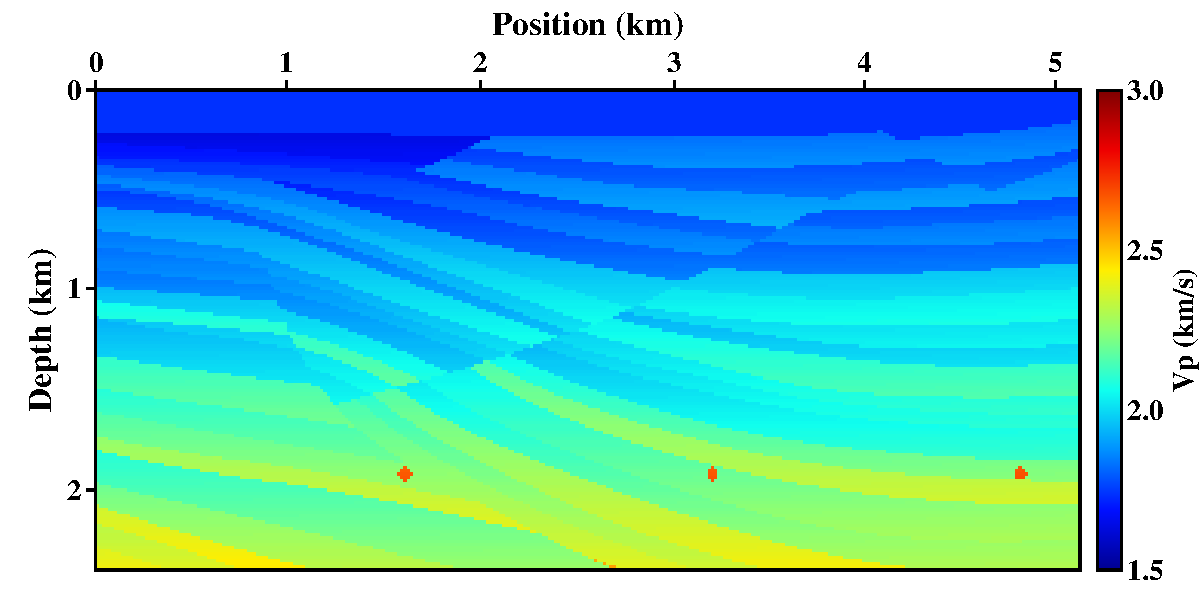
\includegraphics[width=0.48\textwidth]{Figure/chapter03/sigbee2/Fig/cuttruevp.pdf}}
   \subfloat[]{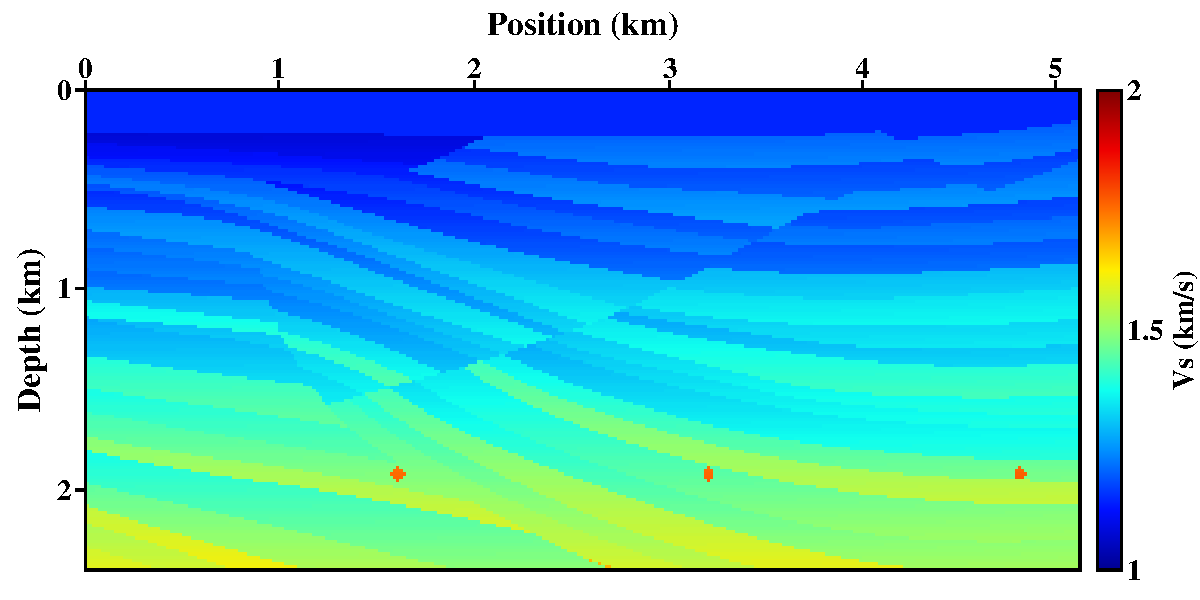
\includegraphics[width=0.48\textwidth]{Figure/chapter03/sigbee2/Fig/cuttruevs.pdf}}\\
   \subfloat[]{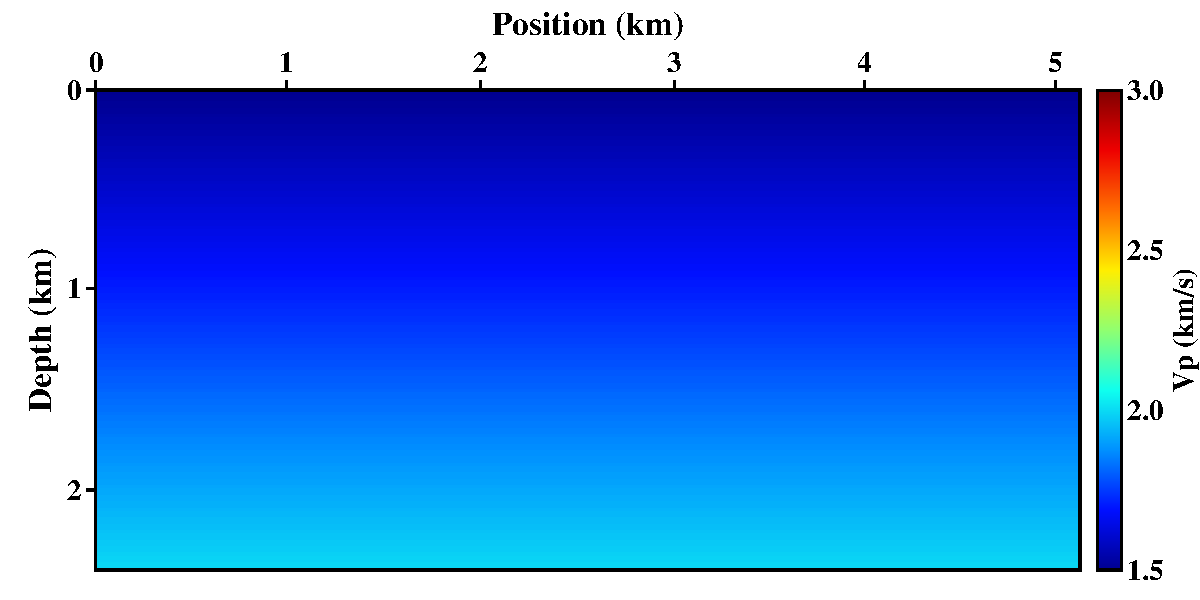
\includegraphics[width=0.48\textwidth]{Figure/chapter03/sigbee2/Fig/cutinitvp.pdf}}
   \subfloat[]{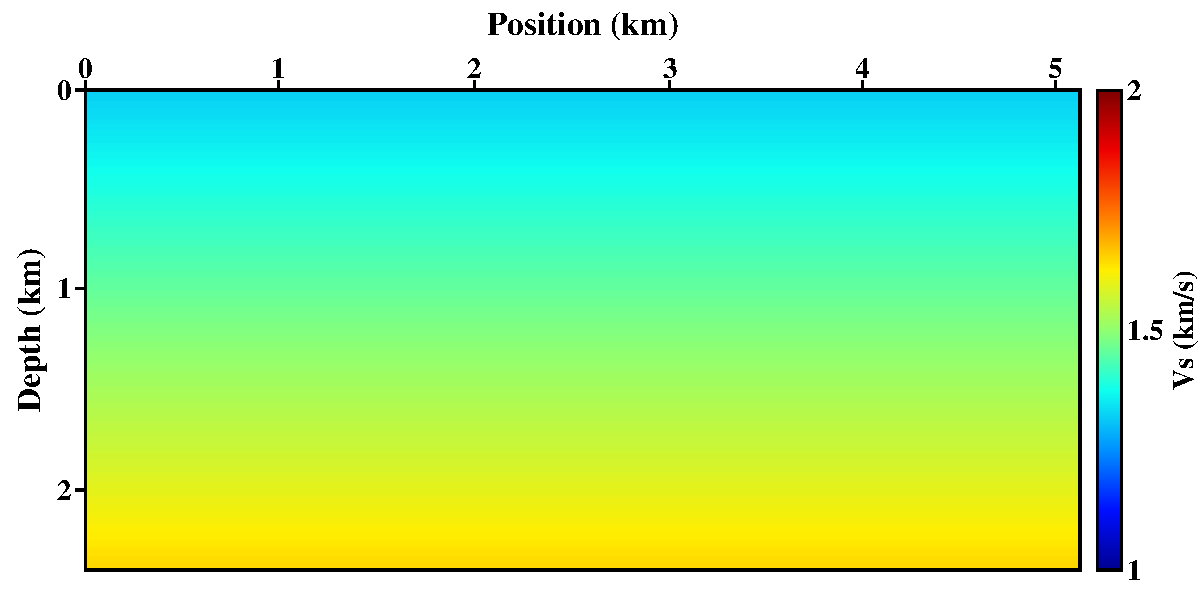
\includegraphics[width=0.48\textwidth]{Figure/chapter03/sigbee2/Fig/cutinitvs.pdf}}
   \caption{Sigbee2A model example. On the top are true models of 
   $V_p$ (a) and $V_s$ (b). On the bottom are initial models of $V_p$ (c) and $V_s$
   (d) linearly increasing with depth. }
   \label{fig:TrueAndInitial}
\end{figure}
我们采用Sigsbee2A模型的一部分来进行实验(如图\ref{fig:TrueAndInitial}a和\ref{fig:TrueAndInitial}b)。$V_s$模型通过一个固定的泊松比来产生。图\ref{fig:TrueAndInitial}c和\ref{fig:TrueAndInitial}d展示了$V_p$和$V_s$的初始模型,其速度值随深度线性增加。我们可以看到初始模型中,$V_p$比真实值偏低而$V_s$则偏高,
但这两者都偏离真实值很远。36炮地面模拟数据均匀的分布在地表,最大偏移距为4km,其震源为主频15Hz的纯P波震源。
\begin{figure}[!htb]
   \centering
   \subfloat[]{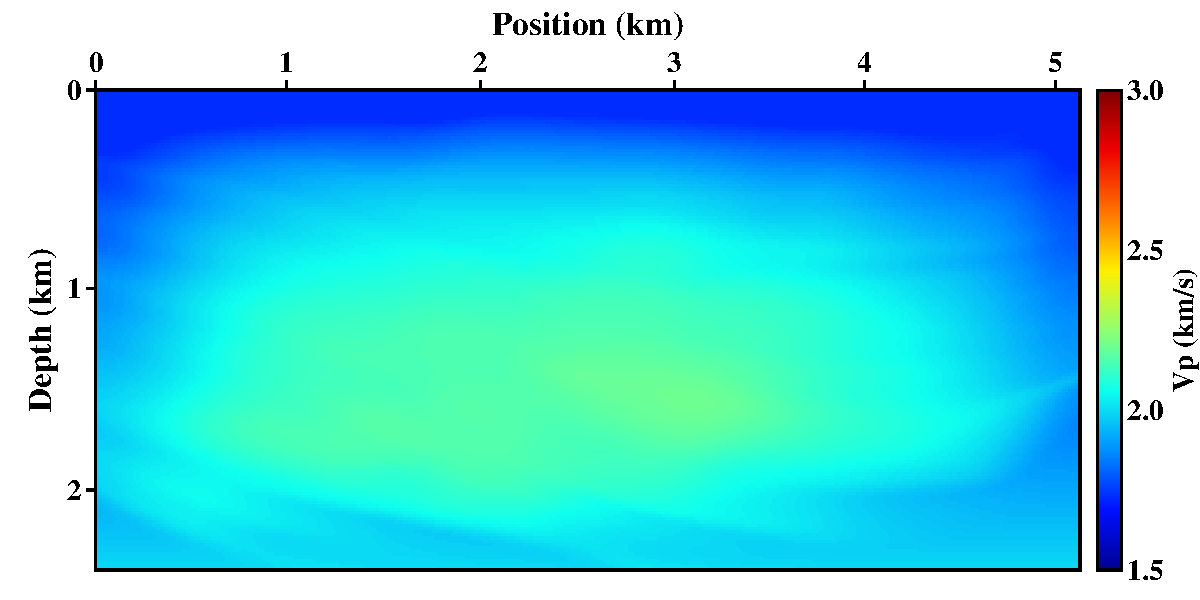
\includegraphics[width=0.48\textwidth]{Figure/chapter03/sigbee2/Fig/newinit3vp.pdf}}
   \subfloat[]{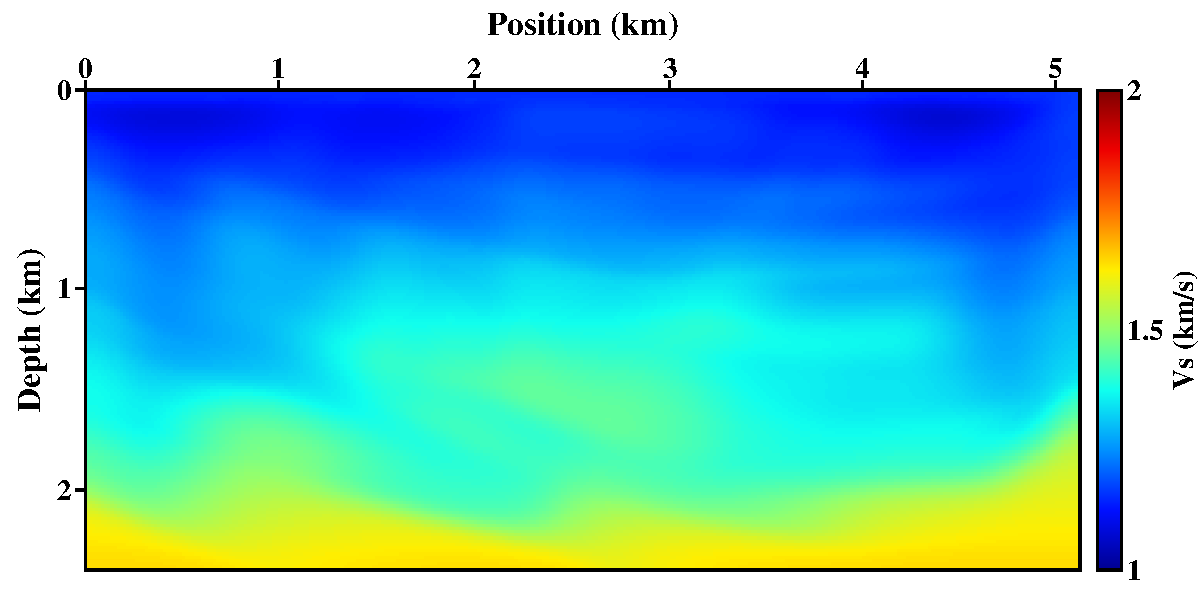
\includegraphics[width=0.48\textwidth]{Figure/chapter03/sigbee2/Fig/newinit3vs.pdf}}\\
   \subfloat[]{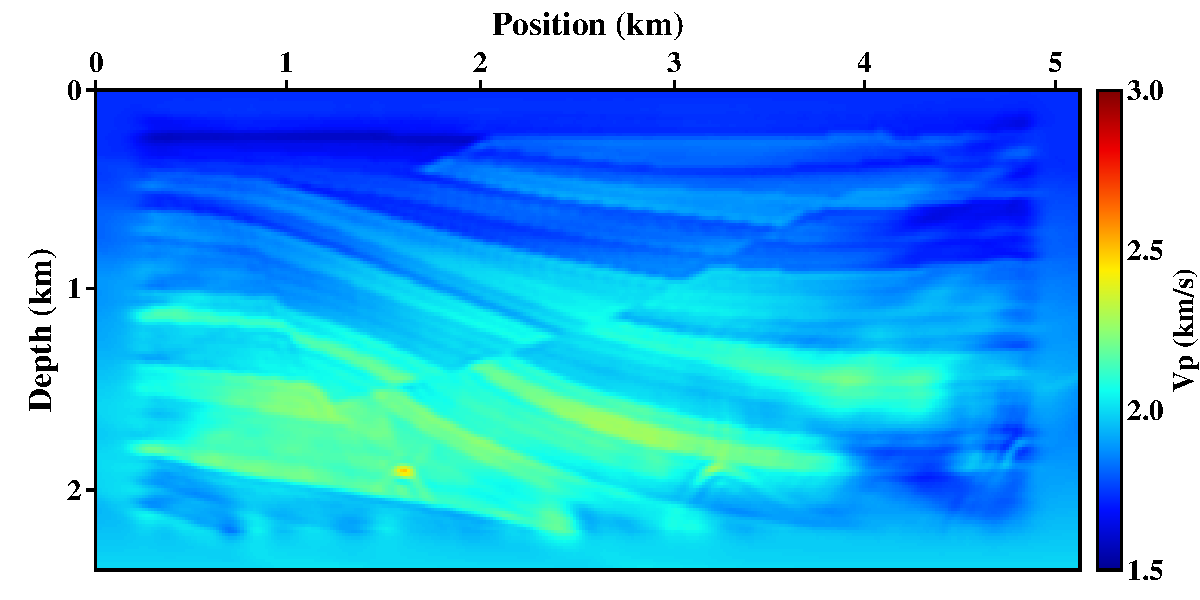
\includegraphics[width=0.48\textwidth]{Figure/chapter03/sigbee2/Fig/nodevp.pdf}}
   \subfloat[]{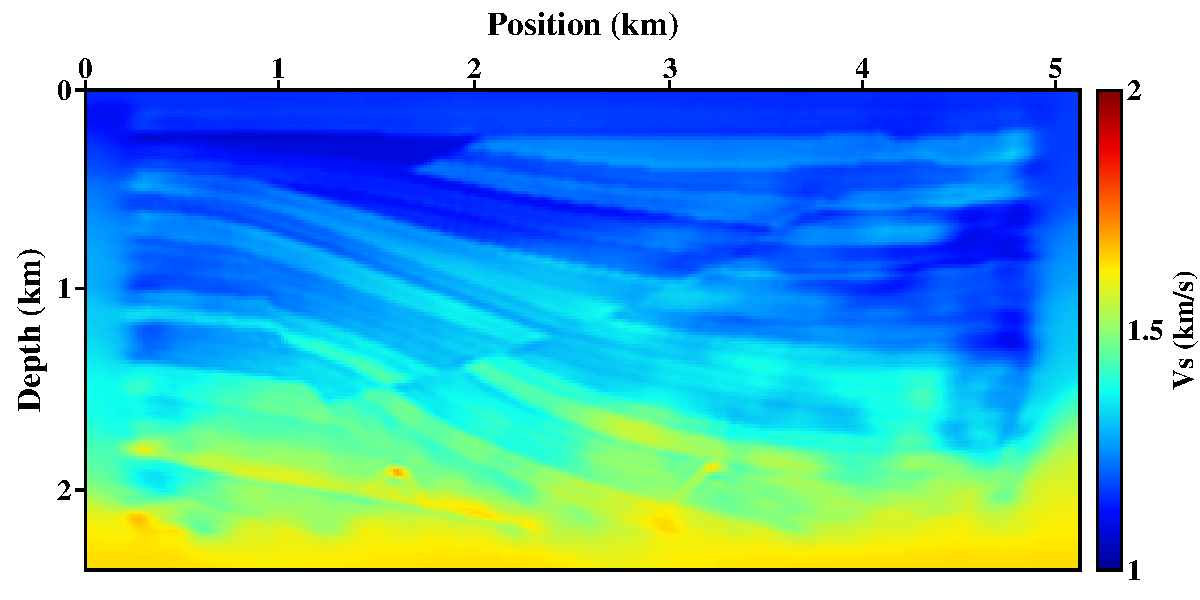
\includegraphics[width=0.48\textwidth]{Figure/chapter03/sigbee2/Fig/nodevs.pdf}}
   \caption{Inverted results of WERTI and EFWI. (a) and (b) are inverted $V_p$ and
       $V_s$ model through two-stage elastic WERTI with the linearly increased models
       as initial models. (c) and (d) are inverted $V_p$ and $V_s$ through EFWI using
   (a) and (b) as starting models.}
   \label{fig:InvertedModel}
\end{figure}
\begin{figure}[!htb]
   \centering
   \subfloat[]{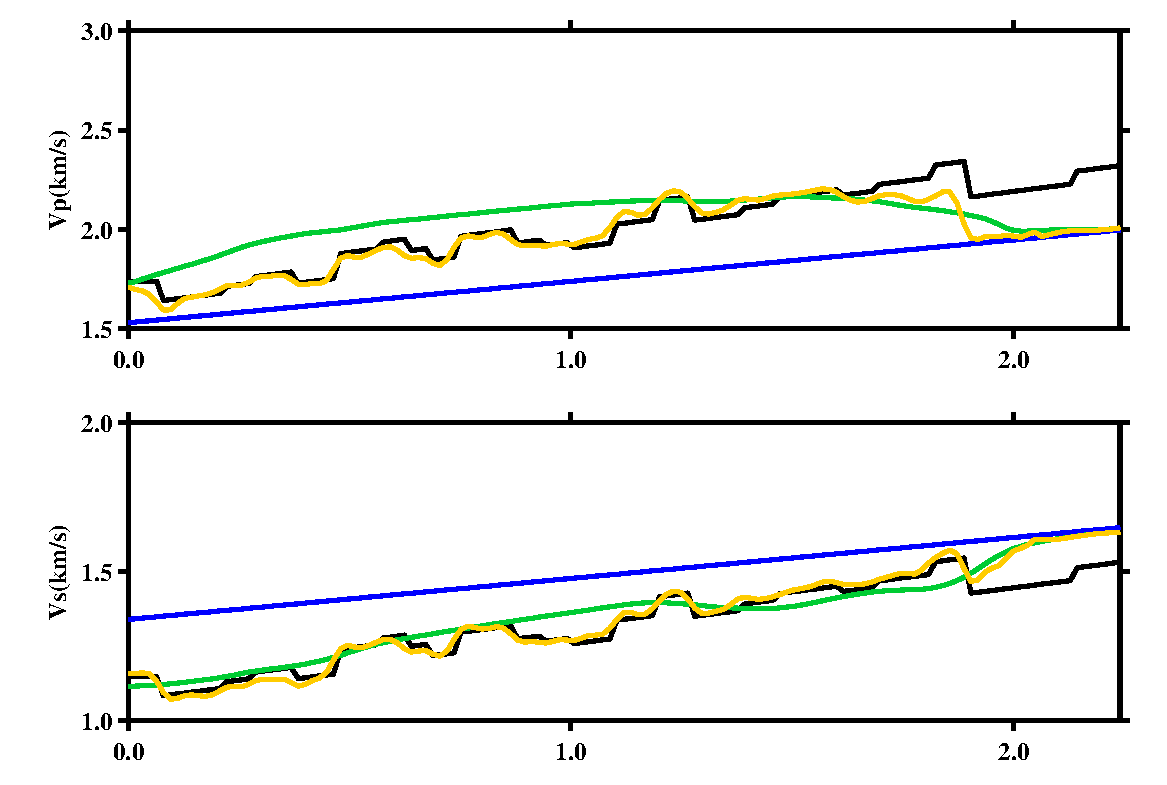
\includegraphics[width=0.48\textwidth]{Figure/chapter03/sigbee2/Fig/1km.pdf}}
   \subfloat[]{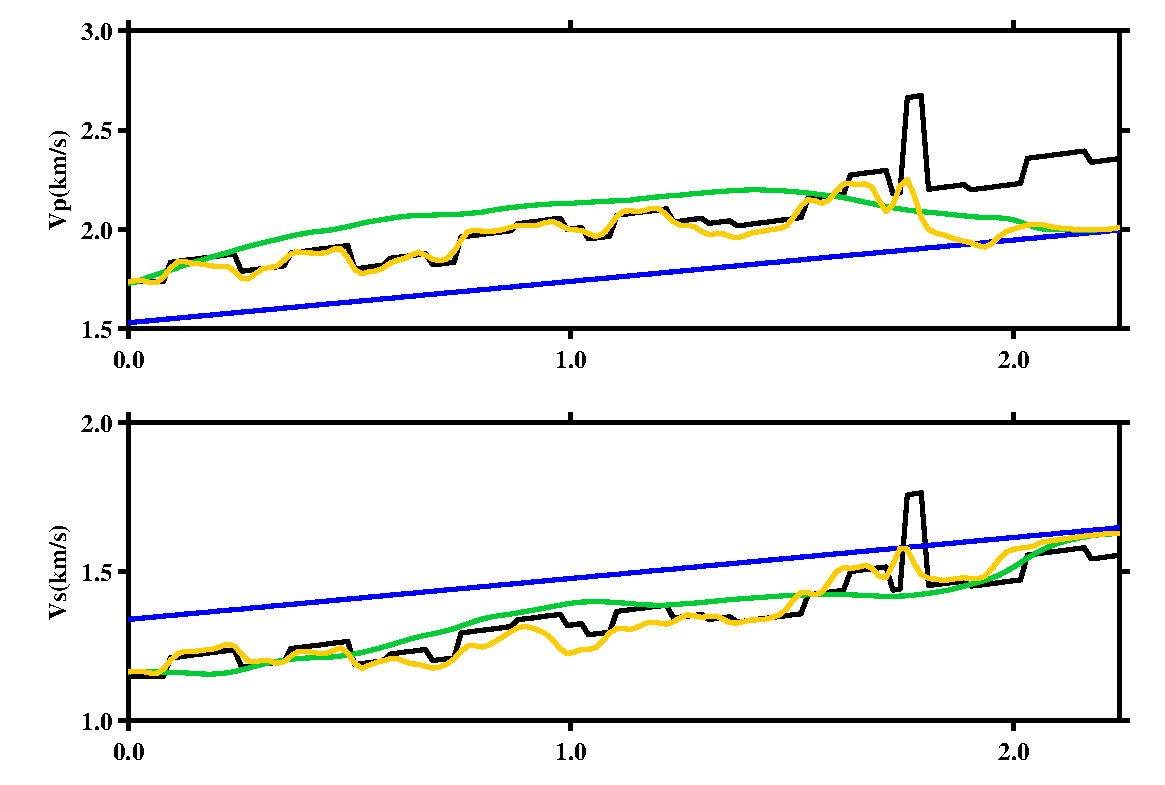
\includegraphics[width=0.48\textwidth]{Figure/chapter03/sigbee2/Fig/3km.pdf}}
   \caption{Vertical profiles of elastic WERTI and EFWI results at 1.4km (a) and
       3km (b). The black and blue lines indicate the true and linearly increased
       initial model. The green and yellow lines indicate the WERTI and EFWI results,
       respectively.
   }
   \label{fig:Profiles}
\end{figure}

图\ref{fig:InvertedModel}a和\ref{fig:InvertedModel}b为弹性WERTI的反演结果。由于线性增加的初始模型偏离真值很远,如果用该模型来进行常规EFWI,将不可避免的
受困于cycle-skipping问题。然而,经过每个阶段40次迭代之后,WERTI可以得到$V_p$和$V_s$较好的背景速度更新。采用WERTI的反演结果作为初始模型,我们重新进行了
常规EFWI反演。如图\ref{fig:InvertedModel}c和\ref{fig:InvertedModel}d所示,$V_p$和$V_s$模型都得到了很好的重建,除了模型右侧一小部分。原因可能是在
地面观测下,模型右侧的反射波覆盖不够导致WERTI不能准确的恢复该区域速度的长波长分量。图\ref{fig:Profiles}也展示了1.5km和3km处的垂向剖面。从图中可以看出,
弹性WERTI能够提供可靠的包含长波长分量的初始模型,并且以此为始模型的EFWI反演结果也与真实值很好的吻合。


%%% Local Variables:
%%% mode: latex
%%% TeX-master: t
%%% End:



\chapter{弹性波波动方程反射FWI走时反演}

\section{引言}
在第1章中,我们知道
EFWI可以提供高精度地下模型参数估计,但是需要有非常好的初始模型。走时反演只利用了走时残差,而走时残差与低波数成分的模型扰动具有更强的线性关系,所以这两者的联系
会更敏感。因此,采用弹性波波动放程反射走时反演(WERTI)来建立P和S波速度的初始模型将会更加稳健且有效,尤其是对深部的宏观结构恢复更有帮助。在弹性介质中,为了区
分P和S波的反射走时,我们将地面地震数据分解为矢量的P-和S-波地震记录。反射P波与S波的走时信息采用Dynamic
image
warping(DIW)的方式来获取。我们首先采用P波走时来反演P波速度,其次采用S波走时来反演S波速度。
在此过程中,我们采用模式解耦来求取预条件的梯度。Sigsbee2A模型的数值实验例子证明了我们的方法可以有效得获取模型长波长信息。

\section{引言}
弹性波全波形反演可以提供高精度的地下模型参数估计,但是也同样受困于多参数反演中的强烈非线性程度以及声波情况下的周波跳跃问题\cite[]{sears:2008,brossier2009}。
Xu et al. (2012)\cite{xu:2012}提出一种反射波波形反演(RWI)的方法,其通过采用偏移/反偏移的方式来预测反射波,从而估计模型中的长波长成分。采用拟合波形的思路,近期
Wu and Alkhalifah (2015)\cite[]{Wu2015b}以及Zhou et al. (2015)\cite[]{Zhou2015}发展了该RWI方法,而Guo and Alkhalifah (2016)\cite{Guo2016}则将该方法扩展到了
弹性介质中。

尽管波形信息能提高反演精度,但是走时信息对模型的低波数成分扰动更敏感,二者之间具有更好的线性关系。所以,采用走时反演来为常规FWI建立合适的含有长波长信息的初始
模型会更加稳健有效\cite[]{Ma2013, Chi2015, Luo2016}。然而在弹性介质中,这中思路会受到限制,因为弹性波场中存在复杂的模式转换,这就导致很难获得单一波模式的走时
信息。在本文中,我们将致力于通过波模式解耦和“动态图像打开”(DIW)\cite[]{Ma2013}来区分出PP和PS的反射走时。之后,我们利用区分出的PP和PS反射走时,通过一个两步
的反演流程来实现WERTI\cite[]{Hale2013}。最后,最后,Sigsbee2A模型的数值实验结果证明了弹性波WERTI方法的有效性。
\section{弹性WERTI方法的目标函数和梯度}
假设在背景弹性介质$c_{ijkl}$中有一个参数扰动$\delta c_{ijkl}$,则背景波场与扰动波场满足以下方程:
\begin{equation}
    \rho \frac{\partial u^2_i}{\partial t^2}  -
    \frac{\partial}{\partial x_j}\left[ 
        c_{ijkl}\frac{\partial u_{k}}{\partial
        x_l}\right]=f_i,
    \label{eq:WE} 
\end{equation}
和
\begin{equation}
    \rho \frac{\partial \delta u^2_i}{\partial t^2}  -
    \frac{\partial}{\partial x_j}\left[ 
        c_{ijkl}\frac{\partial \delta u_{k}}{\partial
        x_l}\right]=\frac{\partial}{\partial x_j}\left[\delta c_{ijkl}\frac{\partial u_{k}}{\partial x_l}\right],
    \label{eq:DeltaWE} 
\end{equation}
其中,$\delta u_i$可以看作是用RTM或其他方法的成像结果,$\delta c_{ijkl}$进行反偏移之后的反射数据。在WERTI中,我们需要使得观测数据$\mathbf{d}^{o}$与模拟数据
$\mathbf{d}^{c}$之间的走时残差最小,则目标函数为:
\begin{equation}
    E=\frac{1}{2}\int\tau^2(\mathbf{x_r},t;\mathbf{x_s})dtd\mathbf{x_r}d\mathbf{x_s},
    \label{eq:Objectivefunction} 
\end{equation}
其中,走时残差$\tau(\mathbf{x_r},t;\mathbf{x_s})$可以通过DIW来获取。通过类似Ma and
Hale (2013)\cite{Ma2013}的推导(见附录\ref{cha:AdjointForEWERTI}),我们可以得到如下梯度公式:
\begin{equation}
    \frac{\partial E}{\partial c_{ijkl}}=-\int (\frac{\partial u_{i}}{\partial
    x_j}\frac{\partial \delta \psi_{k}}{\partial x_l}+\frac{\partial \delta u_{i}}{\partial
    x_j}\frac{\partial \psi_{k}}{\partial x_l}),
    \label{eq:GradientCijkl}
\end{equation}
其中,$\psi_i$和$\delta \psi_i$是共轭波场满足:
\begin{equation}
    \rho \frac{\partial \psi^2_i}{\partial t^2}  -
    \frac{\partial}{\partial x_j}\left[ 
        c_{ijkl}\frac{\partial \psi_{k}}{\partial
        x_l}\right]=\tau(\mathbf{x_r},t;\mathbf{x_s})\frac{\dot{d}^o_i(\mathbf{x_r},t+\tau;\mathbf{x_s})}{h_i(\mathbf{x_r},t;\mathbf{x_s})},
    \label{eq:AdjointWE} 
\end{equation}
和
\begin{equation}
    \rho \frac{\partial \delta \psi^2_i}{\partial t^2}  -
    \frac{\partial}{\partial x_j}\left[ 
        c_{ijkl}\frac{\partial \delta \psi_{k}}{\partial 
        x_l}\right]=\frac{\partial}{\partial x_j}\left[\delta c_{ijkl}\frac{\partial
        \psi_{k}}{\partial x_l}\right], 
    \label{eq:AdjointDeltaWE} 
\end{equation}
上式中$h_i(\mathbf{x_r},t;\mathbf{x_s})=(\dot{d}^o_i(\mathbf{x_r},t+\tau;\mathbf{x_s}))^2-\ddot{d}^o_i(\mathbf{x_r},t+\tau;\mathbf{x_s})
(d^c_i(\mathbf{x_r},t;\mathbf{x_s})-d^o_i(\mathbf{x_r},t+\tau;\mathbf{x_s}))$,而$\dot{d}$则代表$d$在时间方向的导数。在方程\eqref{eq:GradientCijkl}的右端项
中,第一和第二项分别表示震源端和检波点端的反射波路径。之后我们可以通过链式法则来导出P波与S波速度的梯度公式:
\begin{equation}
    \frac{\partial E}{\partial V_p}=2\rho V_p\frac{\partial E}{\partial
        c_{ijkl}}\delta_{ij}\delta_{kl}, \qquad
    \frac{\partial E}{\partial V_s}=2\rho V_s\frac{\partial
    E}{\partial c_{ijkl}}(-2\delta_{ij}\delta_{kl}+\delta_{ik}\delta_{jl}+
    \delta_{il}\delta_{jk}).
    \label{eq:GradientVel}
\end{equation}
\section{弹性波WERTI工作流程}
弹性波介质中,不同模式的转换波,主要是PP与PS同相轴之间,会互相叠加、互相交叉。在用DIW提取走时差的时候,这些交叉点的位置就会变成一些奇异点而给拾取带来很大困难
。因此,如果直接用原始多分量数据的话,拾取到的$\tau(\mathbf{x_r},t;\mathbf{x_s})$就会不准确,这也是为什么式\eqref{eq:AdjointDeltaWE}中的梯度很难直接应用。
为了解决这个问题,我们将观测与模拟地震数据分解为P波与S波两部分。该模式分解只作用于地面地震数据\cite[]{Li2016a},因此我们可以快速地获得每一炮数据分解之后的矢量
P波或S波地震记录。这样,走时残差就可以被分成P波与S波两部分,使得弹性波WERTI变得可行,也即用一个两阶段的流程,先P波阶段后S波阶段。

在P波阶段,主要采用PP反射波来建立P波速度的背景模型。首先,我们从ERTM中获得P波速度的扰动,也即$\delta V_p$。由于在WERTI中我们只考虑走时,所以我们只进行ERTM成像
而不是最小平方ERTM来拟合反射波振幅。因此,目标函数可以变做最小化PP反射波的走时残差:
\begin{equation}
    E_{pp}=\frac{1}{2}\int\tau^2_{pp}(\mathbf{x_r},t;\mathbf{x_s})dtd\mathbf{x_r}d\mathbf{x_s}.
    \label{eq:ObjectivefunctionPP} 
\end{equation}
这样,采用P波记录来计算方程\eqref{eq:AdjointWE}的右端项,并用$\delta V_p$替换方程\eqref{eq:DeltaWE}和\eqref{eq:AdjointDeltaWE}中的$\delta c_{ijkl}$,我们
就可以计算得到$V_p$的梯度, $\frac{\partial E}{\partial V_p}$。

在S波阶段,我们将采用类似的策略但是只利用PS反射波。则目标函数变为:
\begin{equation}
    E_{ps}=\frac{1}{2}\int\tau^2_{ps}(\mathbf{x_r},t;\mathbf{x_s})dtd\mathbf{x_r}d\mathbf{x_s}.
    \label{eq:ObjectivefunctionPS} 
\end{equation}
但是,实现方式与前一阶段策略略有不同。经过P波阶段反演之后,$V_p$的背景速度已经获得了很好的恢复,此时PP波成像结果应该已经比较接近准确位置。而通常情况下,地
下介质中$V_p$与$V_s$的界面是比较一致的。所以,我们推荐采用较为准确的PP成像($\delta V_p$)结果而不是$\delta V_s$来产生PS反射波。此外,在PS反射中,波路径的
震源端只与P波速度相关,因此我们在计算$\frac{\partial E}{\partial V_s}$可以丢掉方程\eqref{eq:GradientCijkl} 右端项的第一部分。并且,波模式分解也会施加在
梯度的计算过程中来确保只有S波能量参与其中:
\begin{equation}
    \frac{\partial E_{ps}}{\partial V_s}=-2\rho V_s
    \int (\frac{\partial \delta u^S_{i}}{\partial
    x_j}\frac{\partial \psi^S_{k}}{\partial x_l})
    (\delta_{ik}\delta_{jl}+
    \delta_{il}\delta_{jk}).
    \label{eq:GradientVel}
\end{equation}
上述梯度与Wang et al. (2015)\cite{Wang2015a}提出的EFWI方法类似。模式解耦可以在$V_s$的反演中降低参数耦合同时也可以压制假象。

\section{局部倾角滤波约束}
WERTI非常类似成像域射线走时层析。而我们知道射线走时层析反问题通常不收敛,很难收敛或者很难收敛获得具有地质意义的模型。
在偏移后,成像结果可以提供地下界面大致的倾角信息,通过此类倾角信息,可以设计预条件算子来沿地层倾角来对反演进行约束,使得反演结果更合理。
采用倾角约束滤波可以加快收敛速度,在很大程度上改善反演结果。由于采用波动方程作为手段,WERTI采用波路径信息来反投影走时残差信息,因而其所面临的挑战要
小于射线走时层析。然而,对于一些照明不足,或者
反射路径覆盖不均匀的区域同样也会出现上述的问题。常规的各向同性的平滑算子很难保证反演收敛到具有地质含义的物理模型。因此,WERTI中采用局部倾角约束同样可以加速
收敛,并获得具有地质意义的反演结果。

Hale(2009)采用结构张量来估计地层倾角。对于2D的图像,结构张量是$2\times2$的矩阵:
\begin{equation}
        \mathbf{S}=
        \begin{pmatrix}
                < s^2_1 > \quad <s_1s_2 >\\
                < s_1s_2 > \quad < s^2_2 >\\
        \end{pmatrix},
        \label{eq:StructureTensor}
\end{equation}
其中$s_1$和$s_2$表示图像垂直和水平方向的方向导数,$<\dot>$表示2D的Gaussian平滑函数。上式对应的特征值问题可以表示为:
\begin{equation}
	\mathbf{S}=\lambda_u\mathbf{u}\mathbf{u}^T+\lambda_v\mathbf{v}\mathbf{v}^T
        \label{eq:EigenValueVector}
\end{equation}
其中,$\lambda_u$和$\lambda_v$分别为特征向量$\mathbf{u}$和$\mathbf{v}$对应的特征值。我们定义$\lambda_u\ge\lambda_v\ge0$,这样的话$\mathbf{u}$指示梯度最大的
方向,也即与线性结构垂直的方向。而话$\mathbf{u}$则指示与线性结构平行的方向。Hale(2009)指出,可以设置$\lambda_u(\mathbf{x})=0$
和$\lambda_v(\mathbf{x})=1$,这样保证图像中每一处平滑都会沿倾角方向。则沿倾角平滑的滤波器可以通过以下方程求解:
\begin{equation}
	(\mathbf{B}^T\mathbf{B}+\mathbf{A}^T\mathbf{S}^{\prime}\mathbf{A})\mathbf{h}=\mathbf{B}^T\mathbf{B}\mathbf{f}
        \label{eq:SparseMatrixSystem}
\end{equation}
其中,$\mathbf{S}^{\prime}$为新构造的结构张量,$\mathbf{B}$和$\mathbf{A}$分别为求和算子以及差分算子对应的矩阵,$\mathbf{f}$为输入图像,$\mathbf{h}$
为输出的平滑后图像。该方程可以通过共轭梯度法快速求解。

\section{数值实验}
\subsection{目标函数性态变化}
\subsection{Sigsbee2A模型}
\begin{figure}
   \centering
   \subfloat[]{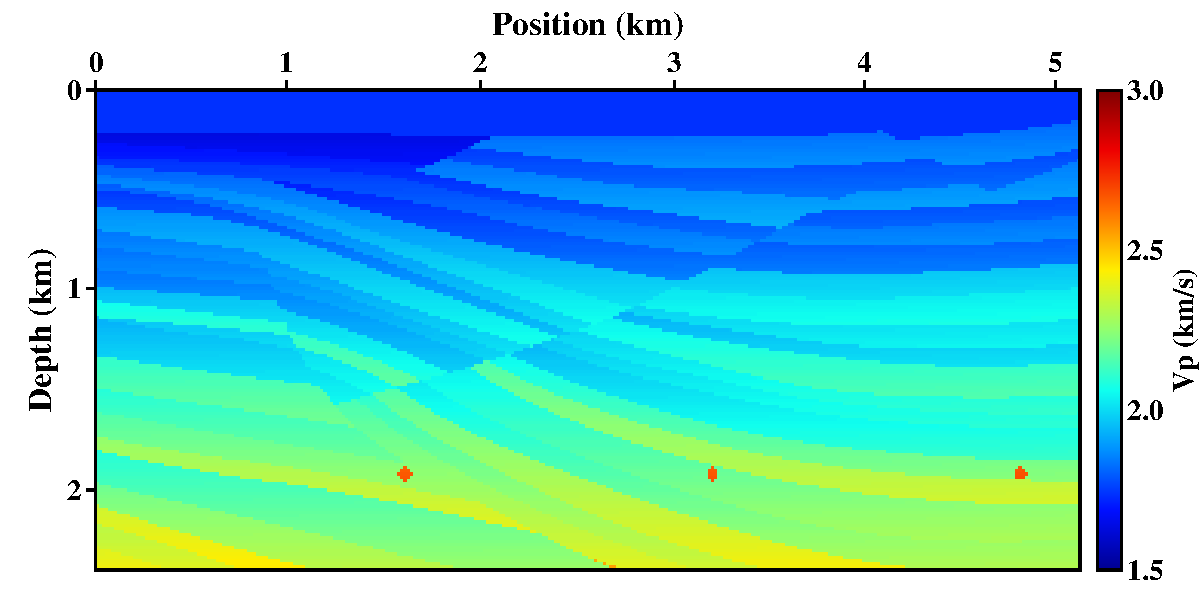
\includegraphics[width=0.48\textwidth]{Figure/chapter03/sigbee2/Fig/cuttruevp.pdf}}
   \subfloat[]{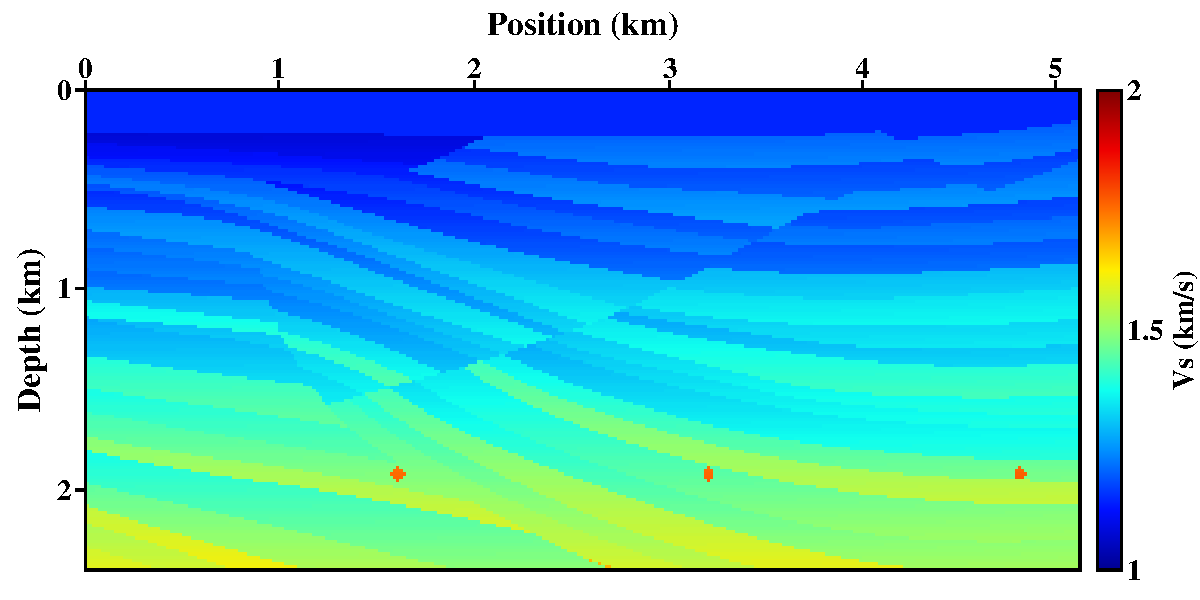
\includegraphics[width=0.48\textwidth]{Figure/chapter03/sigbee2/Fig/cuttruevs.pdf}}\\
   \subfloat[]{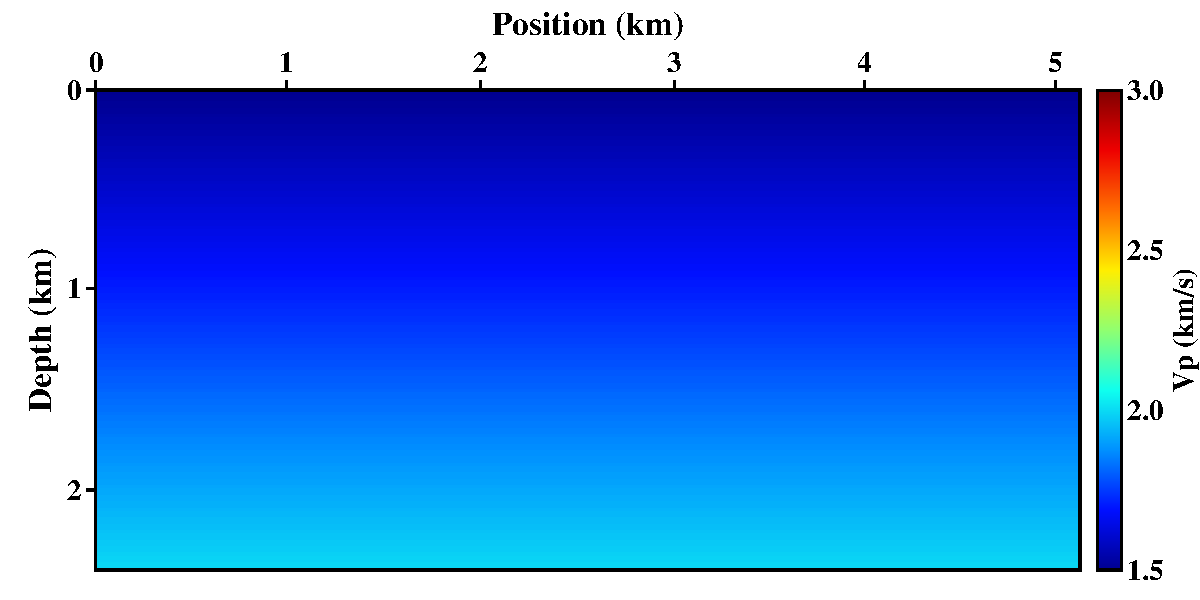
\includegraphics[width=0.48\textwidth]{Figure/chapter03/sigbee2/Fig/cutinitvp.pdf}}
   \subfloat[]{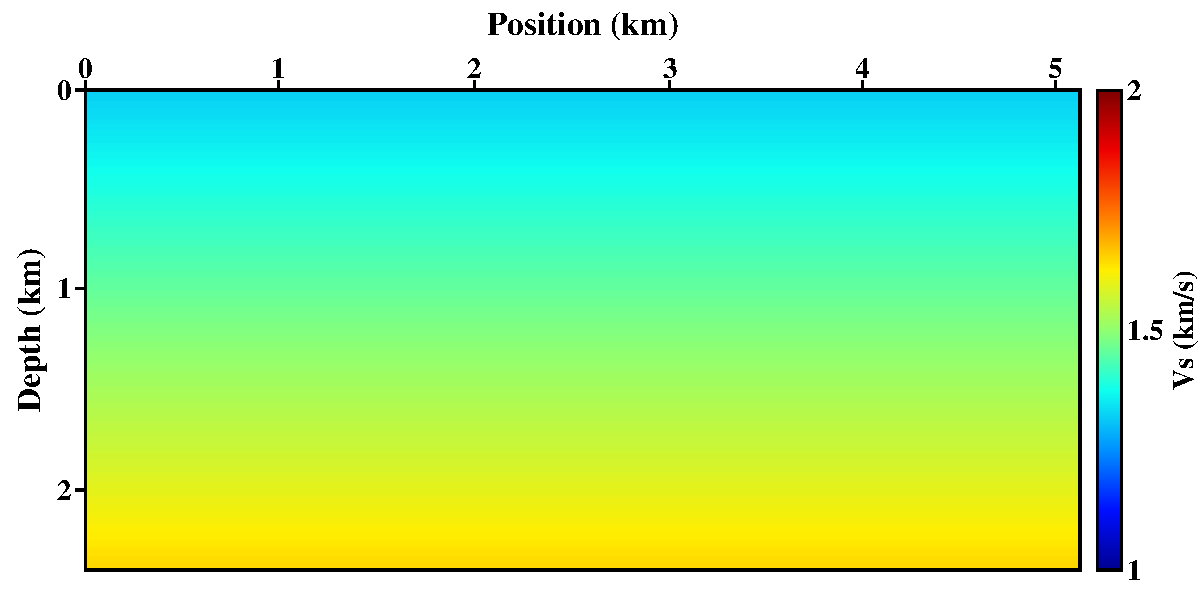
\includegraphics[width=0.48\textwidth]{Figure/chapter03/sigbee2/Fig/cutinitvs.pdf}}
   \caption{Sigbee2A model example. On the top are true models of 
   $V_p$ (a) and $V_s$ (b). On the bottom are initial models of $V_p$ (c) and $V_s$
   (d) linearly increasing with depth. }
   \label{fig:TrueAndInitial}
\end{figure}
我们采用Sigsbee2A模型的一部分来进行实验(如图\ref{fig:TrueAndInitial}a和\ref{fig:TrueAndInitial}b)。$V_s$模型通过一个固定的泊松比来产生。图\ref{fig:TrueAndInitial}c和\ref{fig:TrueAndInitial}d展示了$V_p$和$V_s$的初始模型,其速度值随深度线性增加。我们可以看到初始模型中,$V_p$比真实值偏低而$V_s$则偏高,
但这两者都偏离真实值很远。36炮地面模拟数据均匀的分布在地表,最大偏移距为4km,其震源为主频15Hz的纯P波震源。
\begin{figure}[!htb]
   \centering
   \subfloat[]{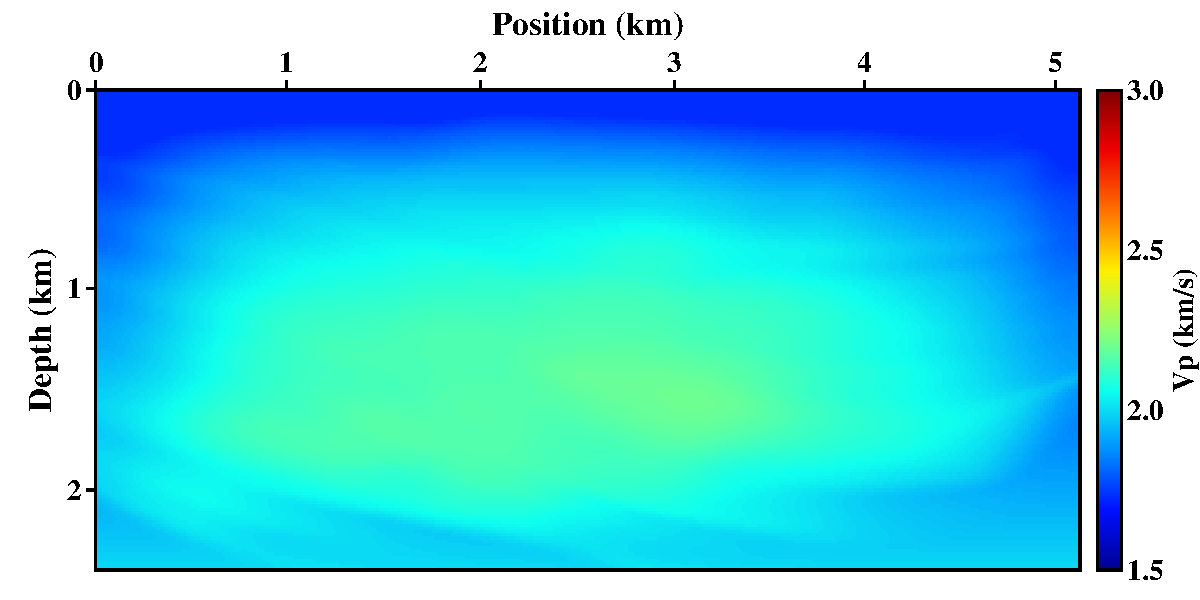
\includegraphics[width=0.48\textwidth]{Figure/chapter03/sigbee2/Fig/newinit3vp.pdf}}
   \subfloat[]{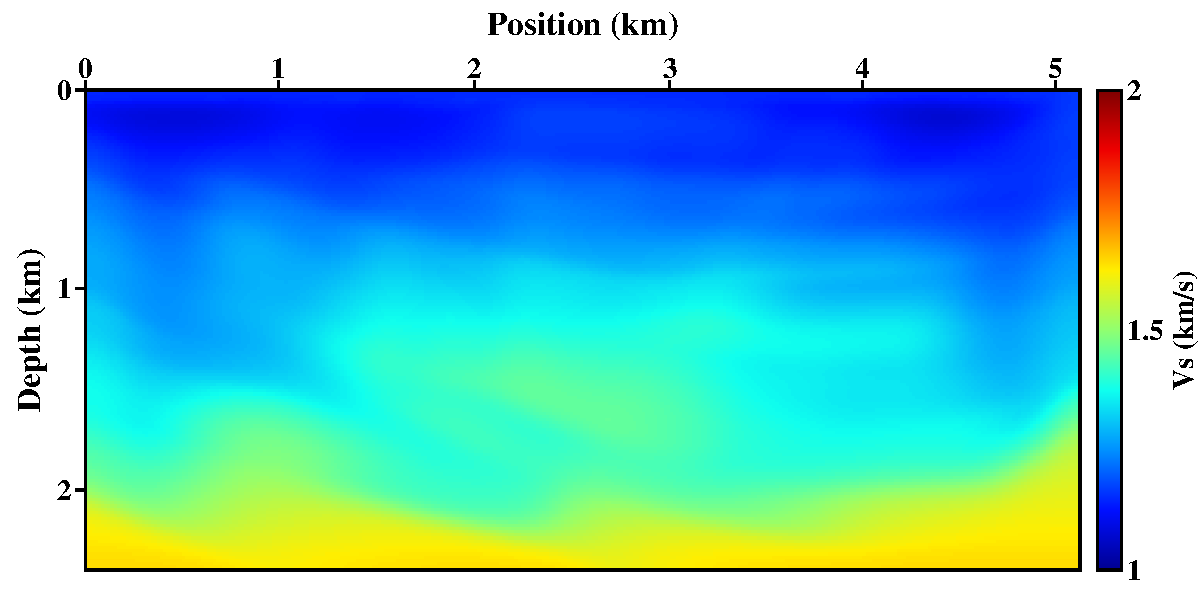
\includegraphics[width=0.48\textwidth]{Figure/chapter03/sigbee2/Fig/newinit3vs.pdf}}\\
   \subfloat[]{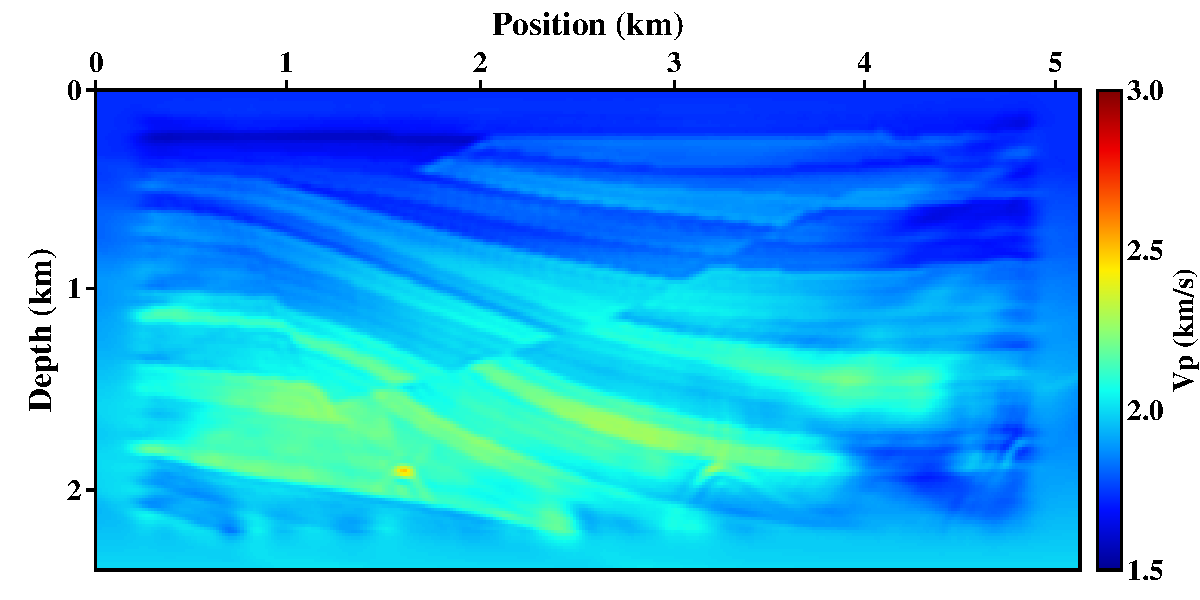
\includegraphics[width=0.48\textwidth]{Figure/chapter03/sigbee2/Fig/nodevp.pdf}}
   \subfloat[]{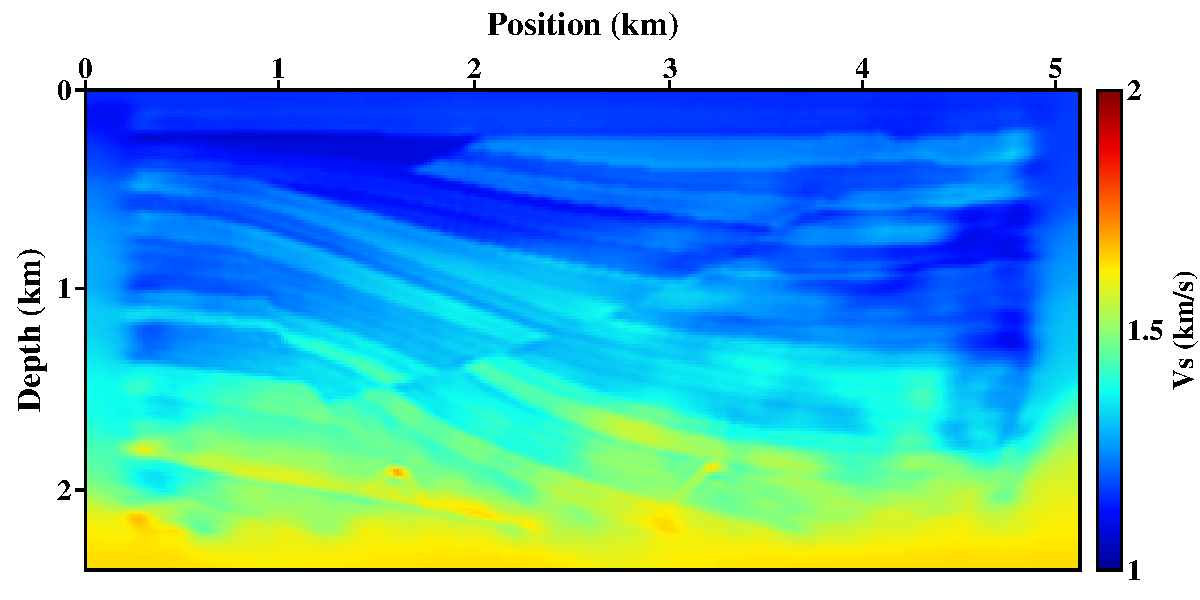
\includegraphics[width=0.48\textwidth]{Figure/chapter03/sigbee2/Fig/nodevs.pdf}}
   \caption{Inverted results of WERTI and EFWI. (a) and (b) are inverted $V_p$ and
       $V_s$ model through two-stage elastic WERTI with the linearly increased models
       as initial models. (c) and (d) are inverted $V_p$ and $V_s$ through EFWI using
   (a) and (b) as starting models.}
   \label{fig:InvertedModel}
\end{figure}
\begin{figure}[!htb]
   \centering
   \subfloat[]{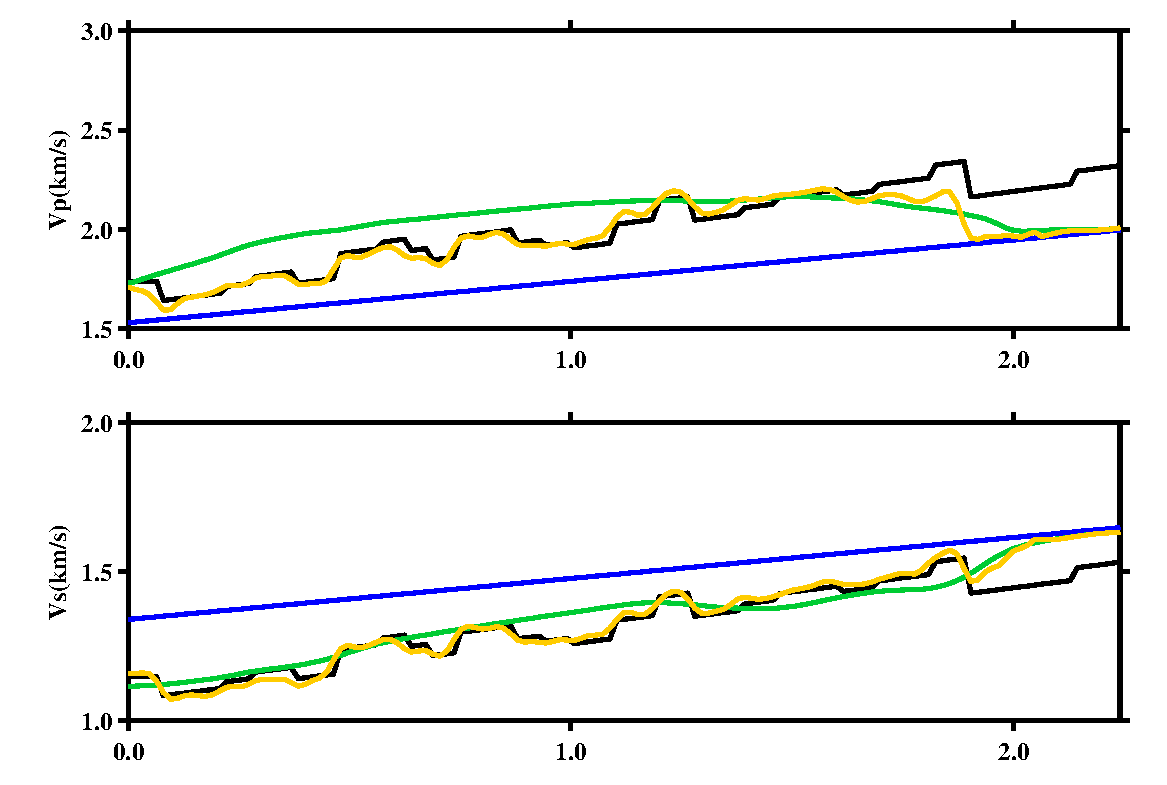
\includegraphics[width=0.48\textwidth]{Figure/chapter03/sigbee2/Fig/1km.pdf}}
   \subfloat[]{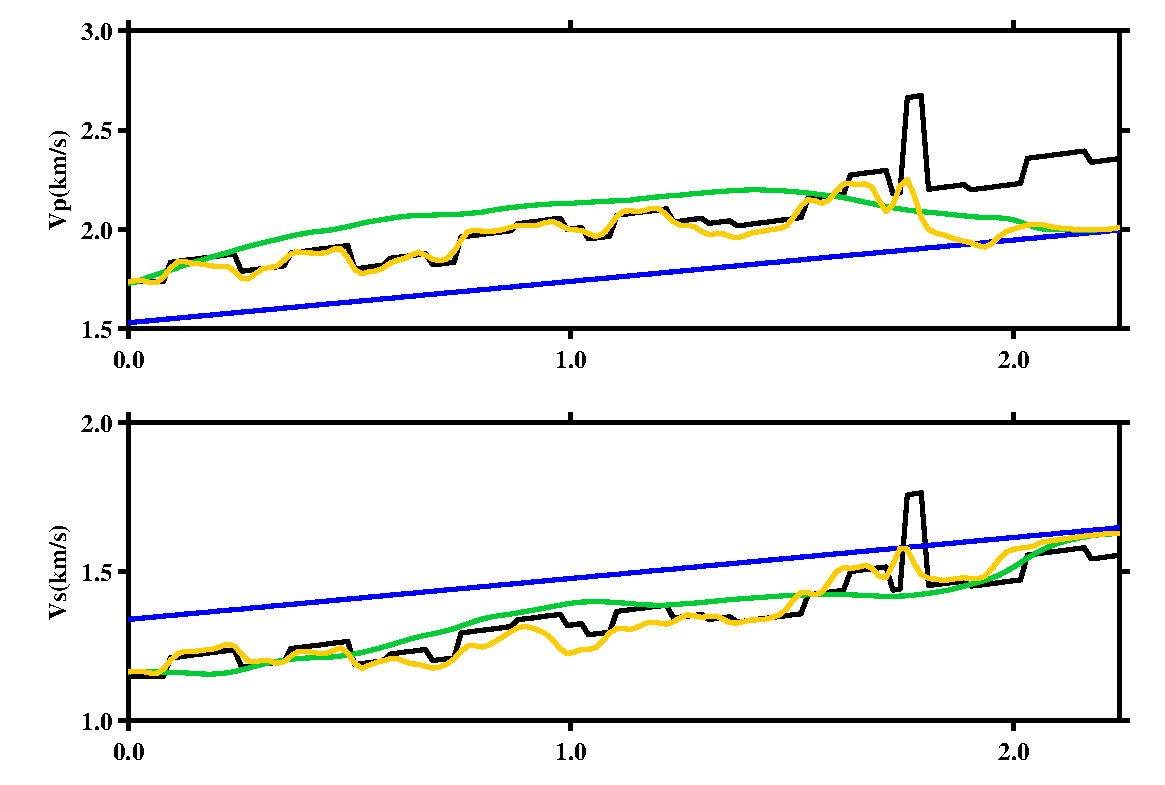
\includegraphics[width=0.48\textwidth]{Figure/chapter03/sigbee2/Fig/3km.pdf}}
   \caption{Vertical profiles of elastic WERTI and EFWI results at 1.4km (a) and
       3km (b). The black and blue lines indicate the true and linearly increased
       initial model. The green and yellow lines indicate the WERTI and EFWI results,
       respectively.
   }
   \label{fig:Profiles}
\end{figure}

图\ref{fig:InvertedModel}a和\ref{fig:InvertedModel}b为弹性WERTI的反演结果。由于线性增加的初始模型偏离真值很远,如果用该模型来进行常规EFWI,将不可避免的
受困于cycle-skipping问题。然而,经过每个阶段40次迭代之后,WERTI可以得到$V_p$和$V_s$较好的背景速度更新。采用WERTI的反演结果作为初始模型,我们重新进行了
常规EFWI反演。如图\ref{fig:InvertedModel}c和\ref{fig:InvertedModel}d所示,$V_p$和$V_s$模型都得到了很好的重建,除了模型右侧一小部分。原因可能是在
地面观测下,模型右侧的反射波覆盖不够导致WERTI不能准确的恢复该区域速度的长波长分量。图\ref{fig:Profiles}也展示了1.5km和3km处的垂向剖面。从图中可以看出,
弹性WERTI能够提供可靠的包含长波长分量的初始模型,并且以此为始模型的EFWI反演结果也与真实值很好的吻合。
\begin{figure}[!htb]
   \centering
   \subfloat[]{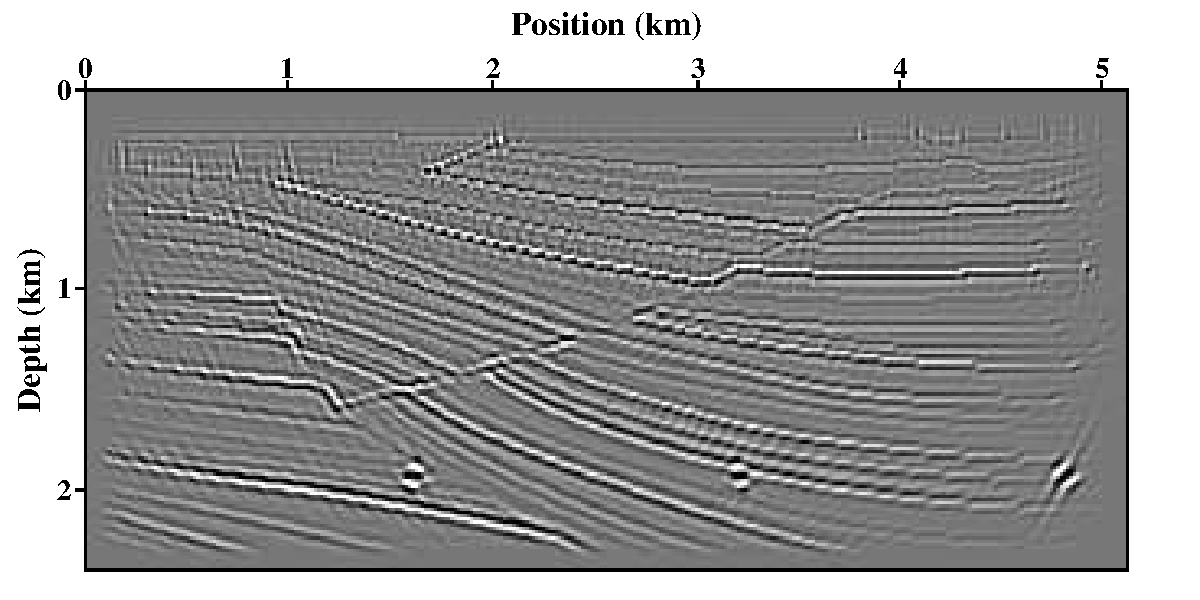
\includegraphics[width=0.48\textwidth]{Figure/chapter03/sigbee2/Fig/cutimage_truevp.pdf}}
   \subfloat[]{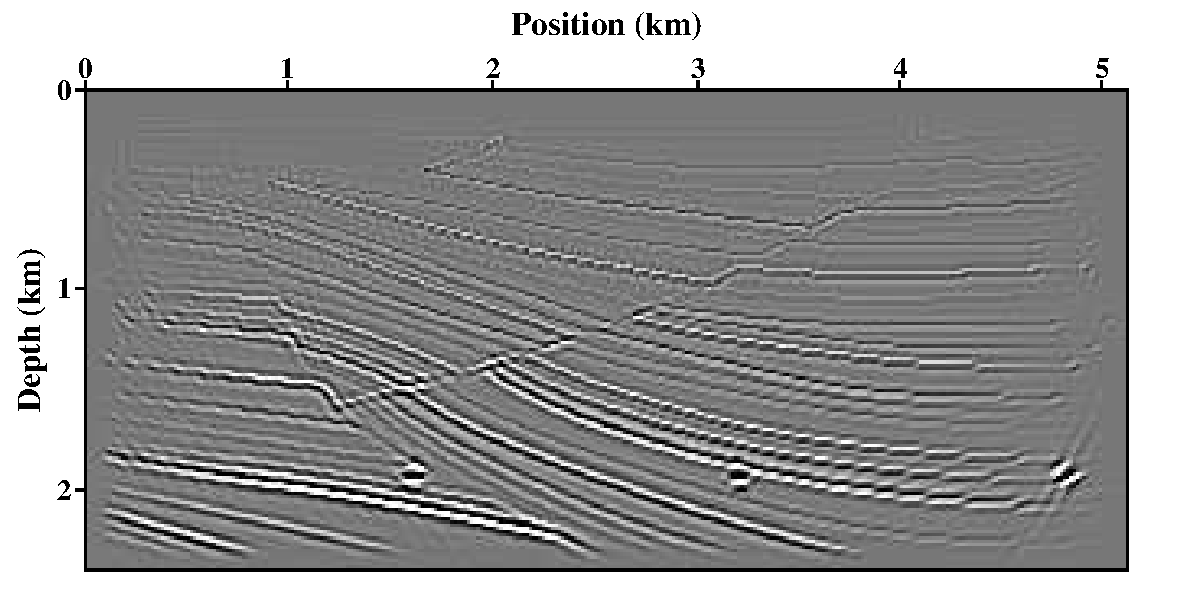
\includegraphics[width=0.48\textwidth]{Figure/chapter03/sigbee2/Fig/cutimage_truevs.pdf}}\\
   \subfloat[]{\includegraphics[width=0.48\textwidth]{Figure/chapter03/sigbee2/Fig/cutimage_initvp.pdf}}
   \subfloat[]{\includegraphics[width=0.48\textwidth]{Figure/chapter03/sigbee2/Fig/cutimage_initvs.pdf}}\\
   \subfloat[]{\includegraphics[width=0.48\textwidth]{Figure/chapter03/sigbee2/Fig/cutimage_wertivp.pdf}}
   \subfloat[]{\includegraphics[width=0.48\textwidth]{Figure/chapter03/sigbee2/Fig/cutimage_wertivs.pdf}}
   \caption{Vertical profiles of elastic WERTI and EFWI results at 1.4km (a) and
       3km (b). The black and blue lines indicate the true and linearly increased
       initial model. The green and yellow lines indicate the WERTI and EFWI results,
       respectively.
   }
   \label{fig:Profiles}
\end{figure}
\begin{figure}[!htb]
   \centering
   \subfloat[]{\includegraphics[width=0.33\textwidth]{Figure/chapter03/sigbee2/Fig/DataPP_true.pdf}}
   \subfloat[]{\includegraphics[width=0.33\textwidth]{Figure/chapter03/sigbee2/Fig/DataPP_init.pdf}}
   \subfloat[]{\includegraphics[width=0.33\textwidth]{Figure/chapter03/sigbee2/Fig/DataPP_werti.pdf}}\\
   \subfloat[]{\includegraphics[width=0.33\textwidth]{Figure/chapter03/sigbee2/Fig/DataPS_true.pdf}}
   \subfloat[]{\includegraphics[width=0.33\textwidth]{Figure/chapter03/sigbee2/Fig/DataPS_init.pdf}}
   \subfloat[]{\includegraphics[width=0.33\textwidth]{Figure/chapter03/sigbee2/Fig/DataPS_werti.pdf}}
   \caption{Vertical profiles of elastic WERTI and EFWI results at 1.4km (a) and
       3km (b). The black and blue lines indicate the true and linearly increased
       initial model. The green and yellow lines indicate the WERTI and EFWI results,
       respectively.
   }
   \label{fig:Profiles}
\end{figure}

\chapter{conclusions}
\backmatter

\makeatother

% 参考文献
%\bibliographystyle{seg}
\bibliographystyle{tongjibib}
%\bibliography{refs}
\bibliography{reference}

% 致谢

%%% Local Variables:
%%% mode: latex
%%% TeX-master: "../main"
%%% End:

\begin{ack}
  啊哈哈哈哈哈

\end{ack}


% 附录
\begin{appendix}
%%% Local Variables:
%%% mode: latex
%%% TeX-master: "../main"
%%% End:

\chapter{外文资料原文}
\label{cha:engorg}
As one of the most widely used techniques in operations research, {\em
  mathematical programming} is defined as a means of maximizing a quantity known
as {\em objective function}, subject to a set of constraints represented by
equations and inequalities. Some known subtopics of mathematical programming are
linear programming, nonlinear programming, multiobjective programming, goal
programming, dynamic programming, and multilevel programming$^{[1]}$.

It is impossible to cover in a single chapter every concept of mathematical
programming. This chapter introduces only the basic concepts and techniques of
mathematical programming such that readers gain an understanding of them
throughout the book$^{[2,3]}$.


\section{Single-Objective Programming}
The general form of single-objective programming (SOP) is written
as follows,
\begin{equation}\tag*{(123)} % 如果附录中的公式不想让它出现在公式索引中,那就请
                             % 用 \tag*{xxxx}
\left\{\begin{array}{l}
\max \,\,f(x)\\[0.1 cm]
\mbox{subject to:} \\ [0.1 cm]
\qquad g_j(x)\le 0,\quad j=1,2,\cdots,p
\end{array}\right.
\end{equation}
which maximizes a real-valued function $f$ of
$x=(x_1,x_2,\cdots,x_n)$ subject to a set of constraints.

\newtheorem{mpdef}{Definition}[chapter]
\begin{mpdef}
In SOP, we call $x$ a decision vector, and
$x_1,x_2,\cdots,x_n$ decision variables. The function
$f$ is called the objective function. The set
\begin{equation}\tag*{(456)} % 这里同理,其它不再一一指定。
S=\left\{x\in\Re^n\bigm|g_j(x)\le 0,\,j=1,2,\cdots,p\right\}
\end{equation}
is called the feasible set. An element $x$ in $S$ is called a
feasible solution.
\end{mpdef}

\newtheorem{mpdefop}[mpdef]{Definition}
\begin{mpdefop}
A feasible solution $x^*$ is called the optimal
solution of SOP if and only if
\begin{equation}
f(x^*)\ge f(x)
\end{equation}
for any feasible solution $x$.
\end{mpdefop}

One of the outstanding contributions to mathematical programming was known as
the Kuhn-Tucker conditions\ref{eq:ktc}. In order to introduce them, let us give
some definitions. An inequality constraint $g_j(x)\le 0$ is said to be active at
a point $x^*$ if $g_j(x^*)=0$. A point $x^*$ satisfying $g_j(x^*)\le 0$ is said
to be regular if the gradient vectors $\nabla g_j(x)$ of all active constraints
are linearly independent.

Let $x^*$ be a regular point of the constraints of SOP and assume that all the
functions $f(x)$ and $g_j(x),j=1,2,\cdots,p$ are differentiable. If $x^*$ is a
local optimal solution, then there exist Lagrange multipliers
$\lambda_j,j=1,2,\cdots,p$ such that the following Kuhn-Tucker conditions hold,
\begin{equation}
\label{eq:ktc}
\left\{\begin{array}{l}
    \nabla f(x^*)-\sum\limits_{j=1}^p\lambda_j\nabla g_j(x^*)=0\\[0.3cm]
    \lambda_jg_j(x^*)=0,\quad j=1,2,\cdots,p\\[0.2cm]
    \lambda_j\ge 0,\quad j=1,2,\cdots,p.
\end{array}\right.
\end{equation}
If all the functions $f(x)$ and $g_j(x),j=1,2,\cdots,p$ are convex and
differentiable, and the point $x^*$ satisfies the Kuhn-Tucker conditions
(\ref{eq:ktc}), then it has been proved that the point $x^*$ is a global optimal
solution of SOP.

\subsection{Linear Programming}
\label{sec:lp}

If the functions $f(x),g_j(x),j=1,2,\cdots,p$ are all linear, then SOP is called
a {\em linear programming}.

The feasible set of linear is always convex. A point $x$ is called an extreme
point of convex set $S$ if $x\in S$ and $x$ cannot be expressed as a convex
combination of two points in $S$. It has been shown that the optimal solution to
linear programming corresponds to an extreme point of its feasible set provided
that the feasible set $S$ is bounded. This fact is the basis of the {\em simplex
  algorithm} which was developed by Dantzig as a very efficient method for
solving linear programming.
\begin{table}[ht]
\centering
  \centering
  \caption*{Table~1\hskip1em This is an example for manually numbered table, which
    would not appear in the list of tables}
  \label{tab:badtabular2}
  \begin{tabular}[c]{|c|m{0.8in}|c|c|c|c|c|}\hline
    \multicolumn{2}{|c|}{Network Topology} & \# of nodes &
    \multicolumn{3}{c|}{\# of clients} & Server \\\hline
    GT-ITM & Waxman Transit-Stub & 600 &
    \multirow{2}{2em}{2\%}&
    \multirow{2}{2em}{10\%}&
    \multirow{2}{2em}{50\%}&
    \multirow{2}{1.2in}{Max. Connectivity}\\\cline{1-3}
    \multicolumn{2}{|c|}{Inet-2.1} & 6000 & & & &\\\hline
    \multirow{2}{1in}{Xue} & Rui  & Ni &\multicolumn{4}{c|}{\multirow{2}*{\tongjithesis}}\\\cline{2-3}
    & \multicolumn{2}{c|}{ABCDEF} &\multicolumn{4}{c|}{} \\\hline
\end{tabular}
\end{table}

Roughly speaking, the simplex algorithm examines only the extreme points of the
feasible set, rather than all feasible points. At first, the simplex algorithm
selects an extreme point as the initial point. The successive extreme point is
selected so as to improve the objective function value. The procedure is
repeated until no improvement in objective function value can be made. The last
extreme point is the optimal solution.

\subsection{Nonlinear Programming}

If at least one of the functions $f(x),g_j(x),j=1,2,\cdots,p$ is nonlinear, then
SOP is called a {\em nonlinear programming}.

A large number of classical optimization methods have been developed to treat
special-structural nonlinear programming based on the mathematical theory
concerned with analyzing the structure of problems.
\begin{figure}[h]
  \centering
  \includegraphics[clip]{tongji-lib-logo.jpg}
  \caption*{Figure~1\hskip1em This is an example for manually numbered figure,
    which would not appear in the list of figures}
  \label{tab:badfigure2}
\end{figure}

Now we consider a nonlinear programming which is confronted solely with
maximizing a real-valued function with domain $\Re^n$.  Whether derivatives are
available or not, the usual strategy is first to select a point in $\Re^n$ which
is thought to be the most likely place where the maximum exists. If there is no
information available on which to base such a selection, a point is chosen at
random. From this first point an attempt is made to construct a sequence of
points, each of which yields an improved objective function value over its
predecessor. The next point to be added to the sequence is chosen by analyzing
the behavior of the function at the previous points. This construction continues
until some termination criterion is met. Methods based upon this strategy are
called {\em ascent methods}, which can be classified as {\em direct methods},
{\em gradient methods}, and {\em Hessian methods} according to the information
about the behavior of objective function $f$. Direct methods require only that
the function can be evaluated at each point. Gradient methods require the
evaluation of first derivatives of $f$. Hessian methods require the evaluation
of second derivatives. In fact, there is no superior method for all
problems. The efficiency of a method is very much dependent upon the objective
function.

\subsection{Integer Programming}

{\em Integer programming} is a special mathematical programming in which all of
the variables are assumed to be only integer values. When there are not only
integer variables but also conventional continuous variables, we call it {\em
  mixed integer programming}. If all the variables are assumed either 0 or 1,
then the problem is termed a {\em zero-one programming}. Although integer
programming can be solved by an {\em exhaustive enumeration} theoretically, it
is impractical to solve realistically sized integer programming problems. The
most successful algorithm so far found to solve integer programming is called
the {\em branch-and-bound enumeration} developed by Balas (1965) and Dakin
(1965). The other technique to integer programming is the {\em cutting plane
  method} developed by Gomory (1959).

\hfill\textit{Uncertain Programming\/}\quad(\textsl{BaoDing Liu, 2006.2})

\section*{References}
\noindent{\itshape NOTE: these references are only for demonstration, they are
  not real citations in the original text.}

\begin{enumerate}[{$[$}1{$]$}]
\item Donald E. Knuth. The \TeX book. Addison-Wesley, 1984. ISBN: 0-201-13448-9
\item Paul W. Abrahams, Karl Berry and Kathryn A. Hargreaves. \TeX\ for the
  Impatient. Addison-Wesley, 1990. ISBN: 0-201-51375-7
\item David Salomon. The advanced \TeX book.  New York : Springer, 1995. ISBN:0-387-94556-3
\end{enumerate}

\chapter{外文资料的调研阅读报告或书面翻译}
\section{单目标规划}
北冥有鱼,其名为鲲。鲲之大,不知其几千里也。化而为鸟,其名为鹏。鹏之背,不知其几
千里也。怒而飞,其翼若垂天之云。是鸟也,海运则将徙于南冥。南冥者,天池也。
\begin{equation}\tag*{(123)}
 p(y|\mathbf{x}) = \frac{p(\mathbf{x},y)}{p(\mathbf{x})}=
\frac{p(\mathbf{x}|y)p(y)}{p(\mathbf{x})}
\end{equation}

吾生也有涯,而知也无涯。以有涯随无涯,殆已!已而为知者,殆而已矣!为善无近名,为
恶无近刑,缘督以为经,可以保身,可以全生,可以养亲,可以尽年。

\subsection{线性规划}
庖丁为文惠君解牛,手之所触,肩之所倚,足之所履,膝之所倚,砉然响然,奏刀騞然,莫
不中音,合于桑林之舞,乃中经首之会。
\begin{table}[ht]
\centering
  \centering
  \caption*{表~1\hskip1em 这是手动编号但不出现在索引中的一个表格例子}
  \label{tab:badtabular3}
  \begin{tabular}[c]{|c|m{0.8in}|c|c|c|c|c|}\hline
    \multicolumn{2}{|c|}{Network Topology} & \# of nodes &
    \multicolumn{3}{c|}{\# of clients} & Server \\\hline
    GT-ITM & Waxman Transit-Stub & 600 &
    \multirow{2}{2em}{2\%}&
    \multirow{2}{2em}{10\%}&
    \multirow{2}{2em}{50\%}&
    \multirow{2}{1.2in}{Max. Connectivity}\\\cline{1-3}
    \multicolumn{2}{|c|}{Inet-2.1} & 6000 & & & &\\\hline
    \multirow{2}{1in}{Xue} & Rui  & Ni &\multicolumn{4}{c|}{\multirow{2}*{\tongjithesis}}\\\cline{2-3}
    & \multicolumn{2}{c|}{ABCDEF} &\multicolumn{4}{c|}{} \\\hline
\end{tabular}
\end{table}

文惠君曰:“嘻,善哉!技盖至此乎?”庖丁释刀对曰:“臣之所好者道也,进乎技矣。始臣之
解牛之时,所见无非全牛者;三年之后,未尝见全牛也;方今之时,臣以神遇而不以目视,
官知止而神欲行。依乎天理,批大郤,导大窾,因其固然。技经肯綮之未尝,而况大坬乎!
良庖岁更刀,割也;族庖月更刀,折也;今臣之刀十九年矣,所解数千牛矣,而刀刃若新发
于硎。彼节者有间而刀刃者无厚,以无厚入有间,恢恢乎其于游刃必有余地矣。是以十九年
而刀刃若新发于硎。虽然,每至于族,吾见其难为,怵然为戒,视为止,行为迟,动刀甚微,
謋然已解,如土委地。提刀而立,为之而四顾,为之踌躇满志,善刀而藏之。”

文惠君曰:“善哉!吾闻庖丁之言,得养生焉。”


\subsection{非线性规划}
孔子与柳下季为友,柳下季之弟名曰盗跖。盗跖从卒九千人,横行天下,侵暴诸侯。穴室枢
户,驱人牛马,取人妇女。贪得忘亲,不顾父母兄弟,不祭先祖。所过之邑,大国守城,小
国入保,万民苦之。孔子谓柳下季曰:“夫为人父者,必能诏其子;为人兄者,必能教其弟。
若父不能诏其子,兄不能教其弟,则无贵父子兄弟之亲矣。今先生,世之才士也,弟为盗
跖,为天下害,而弗能教也,丘窃为先生羞之。丘请为先生往说之。”
\begin{figure}[h]
  \centering
  \includegraphics{hello}
  \caption*{图~1\hskip1em 这是手动编号但不出现索引中的图片的例子}
  \label{tab:badfigure3}
\end{figure}

柳下季曰:“先生言为人父者必能诏其子,为人兄者必能教其弟,若子不听父之诏,弟不受
兄之教,虽今先生之辩,将奈之何哉?且跖之为人也,心如涌泉,意如飘风,强足以距敌,
辩足以饰非。顺其心则喜,逆其心则怒,易辱人以言。先生必无往。”

孔子不听,颜回为驭,子贡为右,往见盗跖。

\subsection{整数规划}
盗跖乃方休卒徒大山之阳,脍人肝而餔之。孔子下车而前,见谒者曰:“鲁人孔丘,闻将军
高义,敬再拜谒者。”谒者入通。盗跖闻之大怒,目如明星,发上指冠,曰:“此夫鲁国之
巧伪人孔丘非邪?为我告之:尔作言造语,妄称文、武,冠枝木之冠,带死牛之胁,多辞缪
说,不耕而食,不织而衣,摇唇鼓舌,擅生是非,以迷天下之主,使天下学士不反其本,妄
作孝弟,而侥幸于封侯富贵者也。子之罪大极重,疾走归!不然,我将以子肝益昼餔之膳。”


\chapter{其它附录}
其它附录的内容可以放到这里,当然如果你愿意,可以把这部分也放到独立的文件中,然后
将其\verb|\input| 到主文件中。

\chapter{共轭状态法推导弹性波WERTI的梯度}
\label{cha:AdjointForEWERTI}
本节中,我们采用Plessix(2006)给出的共轭状态法导出弹性波WERTI的梯度。我们共有三个状态方程其中两个为式\eqref{eq:WE}
和\eqref{eq:DeltaWE}。第三个状态方程来自DIW的优化约束。

我们知道DIW是要找出$\mathbf{\tau}=\tau(\mathbf{x}_r,t;\mathbf{x}_s)$,使得目标函数$D(l)$最小,其中$D(l)$为:
\begin{equation}
	D(\tau)=\frac{1}{2}\int
	d\mathbf{x}_sd\mathbf{x}_r(d_c(\mathbf{x}_r,t;\mathbf{x}_s)-
	d_o(\mathbf{x}_r,t+\tau(\mathbf{x}_r,t;\mathbf{x}_s);\mathbf{x}_s))^2
        \label{eq:Dl}
\end{equation}
而目标函数最小则需要满足:
\begin{equation}
	\frac{\partial D}{\partial \tau}=\int
	d\mathbf{x}_sd\mathbf{x}_r\alpha(\mathbf{x}_r,t;\mathbf{x}_s)=0.
        \label{eq:PartialD}
\end{equation}
其中$\alpha(\mathbf{x}_r,t;\mathbf{x}_s)=\dot{d}_o(\mathbf{x}_r,t+\tau;\mathbf{x}_s)(d_o(\mathbf{x}_r,t+\tau;\mathbf{x}_s)-
d_c(\mathbf{x}_r,t;\mathbf{x}_s))$
偏导数$\frac{\partial D}{\partial
\tau}$一定为0,如果不为0,则我们总能找到一个$\tau$使得$D$变得更小,而这与DIW找到的最小值相矛盾。则式\eqref{eq:PartialD}为
第三个状态方程。我们可以定义增广函数:
\begin{equation}
	\begin{split}
	\mathcal{L}(\mathbf{\tau},\mathbf{u},\mathbf{\psi},\mathbf{\mu},\bar{\mathbf{u}},\bar{\mathbf{\psi}})
	&=\frac{1}{2}\int \tau^2(\mathbf{x}_r,t;\mathbf{x}_s)d\mathbf{x}_sd\mathbf{x}_rdt\\
	&-\int
	\mu(\mathbf{x}_r,t;\mathbf{x}_s)\alpha(\mathbf{x}_r,t;\mathbf{x}_s)d\mathbf{x}_sd\mathbf{x}_rdt\\
	&-\int \bar{{u_i}}\left(\rho\frac{\partial^2
	\psi_i }{\partial t^2}-\frac{\partial}{\partial x_j}(c_{ijkl}\frac{\partial
	\psi_k}{\partial x_l})-\frac{\partial}{\partial x_j}(\delta
	c_{ijkl}\frac{\partial u_k}{\partial x_l})\right)d\mathbf{x}_sd\mathbf{x}_rdt\\
	&-\int \bar{{\psi_i}}\left(\rho\frac{\partial^2 u_i }{\partial
	t^2}-\frac{\partial}{\partial x_j}(c_{ijkl}\frac{\partial u_k}{\partial x_l}) -
	f_i\right)d\mathbf{x}_sd\mathbf{x}_rdt,
	\end{split}
        \label{eq:Lagrangian}
\end{equation}
其中,$\tau(\mathbf{x}_r,t;\mathbf{x}_s)$,$\mathbf{u}$和$\mathbf{\psi}$为状态变量,同时$\mu(\mathbf{x}_r,t;\mathbf{x}_s)$,$\bar{\mathbf{u}}$和$\bar{\mathbf{\psi}}$分别为伴随状态变量,$\bar{\mathbf{u}}$和$\bar{\mathbf{\psi}}$也即反传波场。

伴随状态变量可以通过使增广函数对状态变量偏导数为零来求取,也即使得$\frac{\partial \mathcal{L}}{\partial \mathbf{\tau}}=0$,
$\frac{\partial \mathcal{L}}{\partial \mathbf{u}}=0$和$\frac{\partial \mathcal{L}}{\partial \mathbf{\psi}}=0$。
则
\begin{equation}
	\frac{\partial \mathcal{L}}{\partial \mathbf{\tau}}=\tau(\mathbf{x}_r,t;\mathbf{x}_s)
	-\mu(\mathbf{x}_r,t;\mathbf{x}_s)\frac{\partial \alpha(\mathbf{x}_r,t;\mathbf{x}_s)}{\partial \tau(\mathbf{x}_r,t;\mathbf{x}_s)},
        \label{eq:PartialTau}
\end{equation}
可得
\begin{equation}
	\mu(\mathbf{x}_r,t;\mathbf{x}_s)=\frac{\tau(\mathbf{x}_r,t;\mathbf{x}_s)}{ h_i(\mathbf{x}_r,t;\mathbf{x}_s)},
        \label{eq:AdjointTau}
\end{equation}
其中$h_i(\mathbf{x_r},t;\mathbf{x_s})=(\dot{d}^o_i(\mathbf{x_r},t+\tau;\mathbf{x_s}))^2-\ddot{d}^o_i(\mathbf{x_r},t+\tau;\mathbf{x_s})
(d^c_i(\mathbf{x_r},t;\mathbf{x_s})-d^o_i(\mathbf{x_r},t+\tau;\mathbf{x_s}))$。而$\dot{d}$则代表$d$在时间方向的导数。同时,通过另外两个偏导数方程可得:
\begin{equation}
	\rho\frac{\partial^2 \bar{u}_i }{\partial t^2}
	-\frac{\partial}{\partial x_j}(c_{ijkl}\frac{\partial \bar{u}_k}{\partial x_l})=\mu(\mathbf{x}_r,t;\mathbf{x}_s)
	\dot{d}^o_i(\mathbf{x_r},t+\tau;\mathbf{x_s}),
        \label{eq:PartialU}
\end{equation}
和
\begin{equation}
	\rho\frac{\partial^2 \bar{\psi}_i }{\partial t^2}
	-\frac{\partial}{\partial x_j}(c_{ijkl}\frac{\partial \bar{\psi}_k}{\partial x_l})=
	\frac{\partial}{\partial x_j}(\delta c_{ijkl}\frac{\partial \bar{u}_k}{\partial x_l}).
        \label{eq:PartialPsi}
\end{equation}
这样就可以求得梯度:
\begin{equation}
	\frac{\partial \mathcal{L}}{\partial c_{ijkl}}=
    \frac{\partial E}{\partial c_{ijkl}}=-\int (\frac{\partial u_{i}}{\partial
    x_j}\frac{\partial \bar{\psi}_{k}}{\partial x_l}+\frac{\partial \bar{u}_{i}}{\partial
    x_j}\frac{\partial \psi_{k}}{\partial x_l}),
    \label{eq:GradientCijkl1}
\end{equation}


\end{appendix}

% 个人简历
\begin{resume}

  \resumeitem{个人简历}

  王腾飞,男,汉族,1990年2月出生于河南省襄城县。

  2007年9月,考入同济大学海洋与地球科学学院。

  2011年6月获地球物理学学士学位。

  2011年9月,免试直接攻读同济大学固体地球物理学博士学位至今。

  \resumeitem{已发表期刊论文} % 发表的和录用的合在一起

  \begin{enumerate}[{[}1{]}]
	  \item {\bf{Tengfei Wang}}  and Jiubing Cheng, 2017, Elastic full waveform inversion
		  based on mode decomposition: the approach and mechanism. 
		  \emph{Geophysical Journal International}, 209, 606–622.
	  \item
		  程玖兵,陈茂根,{\bf{王腾飞}},康玮,2014,各向异性介质qP波传播描述II:分离纯模式标量波. \emph{地球物理学报},
	  57(10),3389-3401.
  \item  程玖兵,康玮,{\bf{王腾飞}}, 2013,
  各向异性介质qP波传播描述I:伪纯模式波动方程. \emph{地球物理学报},
	  56(10), 3474-3486.
  \item  Cheng Jiubing, {\bf{Wang Tengfei}}, Wang Chenlong, and Geng Jianhua, 2012, Azimuth-preserved local
	  angle-domain prestack time migration in isotropic, vertical transversely isotropic and
	  azimuthally anisotropic media. \emph{Geophysics}, 77, 2, S51-S64.
  \end{enumerate}

  \resumeitem{已发表会议论文} % 有就写,没有就删除
  \begin{enumerate}[{[}1{]}]
	  \item {\bf{Wang Tengfei}}, Jiubing Cheng and Chenlong Wang, 2017, Elastic wave-equation reflection
		  traveltime inversion using dynamic warping and wave mode decomposition. \emph{79th EAGE
		  Conference \& Exhibition 2017}, Paris, France.
	  \item {\bf{Wang Tengfei}} and Jiubing Cheng, 2016, Comparison between mode decomposition based and
		  Gaussian Newton methods in elastic full waveform inversion. \emph{ 78th EAGE Conference \&
		  Exhibition}, Vienna, Austria.
	  \item Yang T, {\bf{Wang T}}, Cheng J, 2016, Regularization method of tomography based on the ADCIGs
		  with geologic dip information. \emph{SEG International Geophysical
		  Conference} Beijing, China.
	  \item {\bf{Wang Tengfei}}, Jiubing Cheng and Chenlong Wang, 2015, Elastic wave mode decoupling for
		  full waveform inversion. \emph{77th EAGE Conference \& Exhibition}, Mardrid, Spain.
	  \item {\bf{Wang Tengfei}} and Jiubing Cheng, 2015, Elastic wave mode decoupling for full waveform
		  inversion. \emph{85th SEG Annual International Meeting}, Expanded Abstracts.
	  \item   {\bf{Wang T}}, Kang W, Cheng J, 2014, Migration velocity model building using local angle domain non-
		  linear tomography. \emph{International Geophysical Conference and Exposition}, 
		  Beijing, China. 
	  \item Wang Chenlong, Cheng Jiubing and {\bf{Wang Tengfei}}, 2014, Local angle domain elastic reverse
		  time migration in TI media. \emph{76th EAGE Conference \& Exhibition}, Amsterdam,
		  Netherlands. 
	  \item {\bf{Wang Tengfei}}, Cheng Jiubing and Kang Wei, 2012, Pure mode modeling and reverse-time
		  migration of P-wave in HTI and orthorhombic media.\emph{82nd Ann.
		  Internat Mtg. SEG}, Expanded Abstracts, Las Vegas, USA.
			  
  \end{enumerate}
\end{resume}


\end{document}
